%%%%%%%% CST-S2TT paper draft (ICML 2026 style; switch to the ICML 2027 style files when they are released) %%%%%%%%
% Build:  tectonic -X compile main.tex      (or: latexmk -pdf main.tex)
% Pending numbers: \tbd (table cells, blank by default) and \tbdtext (running text, always visible).
% Draft marks: set \showpendingtrue below to show a dot in every pending table cell;
%              set \showdraftnotesfalse to hide \draftnote{...} remarks.

\documentclass{article}

\usepackage{microtype}
\usepackage{graphicx}
\usepackage{subcaption}
\usepackage{booktabs}
\usepackage{hyperref}
\newcommand{\theHalgorithm}{\arabic{algorithm}}

% Initial blind version for review:
\usepackage{icml2026}
% Tectonic/XeTeX builds only: use the same OT1 Type 1 Times fonts as pdfLaTeX
% (otherwise XeTeX falls back to Latin Modern). No effect under pdfLaTeX.
\usepackage{iftex}
\ifXeTeX\usepackage[OT1]{fontenc}\fi
% Preprint:      \usepackage[preprint]{icml2026}
% Camera-ready:  \usepackage[accepted]{icml2026}

\usepackage{amsmath}
\usepackage{amssymb}
\usepackage{mathtools}
\usepackage{amsthm}
\usepackage[capitalize,noabbrev]{cleveref}

% ---------------------------------------------------------------------------
% Project macros
% ---------------------------------------------------------------------------
\usepackage{xspace}
\usepackage{xcolor}
\usepackage{multirow}
\usepackage{makecell}
\usepackage{pifont}

% Pending numbers. Table cells that wait for experiments use \tbd.
% By default the cell stays blank (as requested); compile with \showpendingtrue
% (see main.tex) to mark every pending cell with a grey dot while drafting.
\newif\ifshowpending
\showpendingfalse
\newcommand{\tbd}{\ifshowpending\textcolor{black!35}{$\cdot$}\fi}
% Pending number inside running text: always visible so that it cannot be missed.
\newcommand{\tbdtext}[1][]{\textcolor{red!70!black}{[TBD#1]}}
% Preliminary numbers (measured, but to be re-run under the final protocol).
\newcommand{\prelim}[1]{#1$^{\dagger}$}

% Names
\newcommand{\task}{CST\xspace}
\newcommand{\taskfull}{conversational simultaneous speech-to-text translation\xspace}
\newcommand{\bench}{CST-Bench\xspace}
\newcommand{\syn}{CST-Bench-Syn\xspace}
\newcommand{\taxi}{CST-Bench-TAXI\xspace}
\newcommand{\model}{\textsc{Model}\xspace}   % placeholder name of our model
\newcommand{\scorer}{\texttt{cstbench eval}\xspace}

% Directions and languages
\newcommand{\dir}[2]{#1$\rightarrow$#2}
\newcommand{\pair}[2]{#1$\leftrightarrow$#2}
% \newcommand refuses names that start with "end", hence \def for \ende.
\def\ende{\dir{En}{De}\xspace}
\newcommand{\deen}{\dir{De}{En}\xspace}
\newcommand{\enko}{\dir{En}{Ko}\xspace}
\newcommand{\koen}{\dir{Ko}{En}\xspace}

% Metrics
\newcommand{\laal}{StreamLAAL\xspace}
\newcommand{\eo}{EndOffset\xspace}

% Marks
\newcommand{\cmark}{\ding{51}}
\newcommand{\xmark}{\ding{55}}
\newcommand{\pmark}{$\circ$}   % partial / not reported


% Draft switches
%\showpendingtrue
\newif\ifshowdraftnotes
\showdraftnotestrue
\newcommand{\draftnote}[1]{\ifshowdraftnotes{\color{blue!60!black}\footnotesize[\textit{Draft: #1}]}\fi}

\theoremstyle{definition}
\newtheorem{definition}{Definition}

\icmltitlerunning{Who Speaks, Which Way, and When? Simultaneous Speech Translation of Two-Language Conversations}

\begin{document}

\twocolumn[
  \icmltitle{Who Speaks, Which Way, and When?\texorpdfstring{\\}{ }%
    Simultaneous Speech Translation of Two-Language Conversations}

  \icmlsetsymbol{equal}{*}
  \begin{icmlauthorlist}
    \icmlauthor{Anonymous Author(s)}{anon}
  \end{icmlauthorlist}
  \icmlaffiliation{anon}{Anonymous Institution}
  \icmlcorrespondingauthor{Anonymous Author(s)}{anonymous@example.com}

  \icmlkeywords{simultaneous speech translation, conversational speech, streaming speech LLM, benchmark, diarization}

  \vskip 0.3in
]

\printAffiliationsAndNotice{}

% =====================================================================
% Abstract (one paragraph, six sentences, at most 200 words by
% wordcount.py). No preliminary numbers here: every result is \tbdtext
% until its experiment is final. The result templates follow Sec. 6:
% the COMET loss and its split into turn segmentation and routing
% (Sec. 6.3, tab:factorial; COMET points, not percentages), wrong-direction
% words under L1 (fig:gap), the oracle-gap recovery R of the same pipeline
% at a median EndOffset (Sec. 6.1), and Kendall's tau (Sec. 6.7).
% No coupling claim here: the decoupled twin and the same-backbone cascade
% test it (Sec. 6.6).
% =====================================================================
\begin{abstract}
Simultaneous speech translation mostly assumes one speaker and one fixed direction, but a device interpreting between two people who share no language hears both in one mono stream and must decide online who speaks, which way to translate, and when to commit text it cannot retract.
We formalise this task, \taskfull (\task), and introduce \bench, which renders two-language dialogues as continuous single-channel sessions with natural gaps, translation-mediated gaps or turn-end overlap.
It pairs 86 German--English telephone dialogues (real speech, synthetic timing, 640 human-translated turns), released as deterministic build scripts, with an evaluation-only synthetic English--German and Korean--English track.
Its scorer, tested by controlled perturbations, reports per-direction quality, within-turn lag, the listener's wait after each turn, switch latency and wrong-direction output, plus speaker-attributed transcription and diarization errors; Kendall's $\tau$ between system rankings on synthetic and real sessions is \tbdtext{}.
Without oracle segmentation, the best open pipeline loses \tbdtext{} COMET (\tbdtext{} to turn segmentation, \tbdtext{} to routing) and, under turn-end overlap, emits \tbdtext{}\% wrong-direction words.
Our open streaming speech LLM, \model, writes speaker-tagged transcripts and direction-tagged translations into one token stream on an 80\,ms clock and learns to commit translations at alignment-verified meaning units; without oracle input, it recovers \tbdtext{}\% of this loss at a median wait of \tbdtext{}\,s.
\draftnote{planned; the synthetic track, the overlap renders, most scorer modules and \model beyond its streaming ASR backbone are not built yet, and all results are pending}
\end{abstract}

% =====================================================================
% Section 1: introduction (~1.4 columns of text + Fig. 1).
% Fig. 1 (fig:task) is defined at the start of the section so that it
% floats to the top of page 2. The closest systems (JSTAR, DiariST,
% STAC-ST, Seed LiveInterpret 2.0) are introduced here; Sec. 2 and
% Table 1 (tab:positioning) give the details.
% =====================================================================
\section{Introduction}\label{sec:intro}

\begin{figure*}[t]
  \centering
  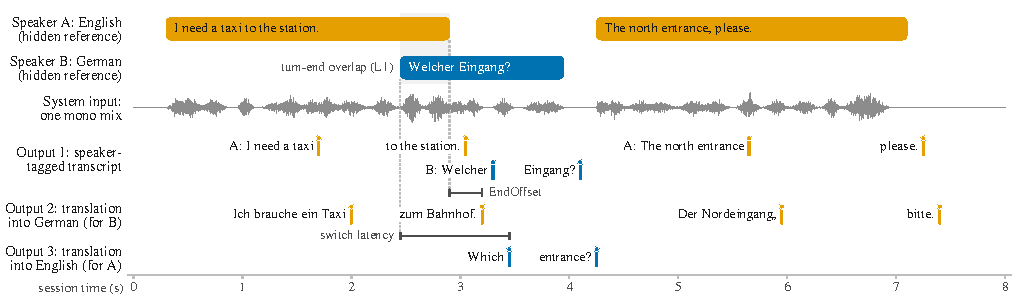
\includegraphics[width=\textwidth]{figures/fig1_task.pdf}
  \caption{\task on one mono stream (illustrative; invented utterances). Speakers A (English) and B (German) share one device. The system hears only the mix and must emit, without retraction, translations into each listener's language, choosing the direction itself, and may also emit a speaker-tagged transcript (Output 1). Ticks mark committed pieces at their emission time, coloured by the speaker whose speech they render. \eo (\emph{end offset}): time from the end of a turn to the last word of its translation, i.e., how long the listener waits. \emph{Switch latency}: time from the start of a turn in the new direction to the first word of its translation. Grey band: turn-end overlap (condition L1). Reference turns are hidden from the system and used only for scoring (\cref{sec:bench} defines the metrics).}
  \label{fig:task}
\end{figure*}

Two people who share no language can talk through a device that translates both sides, a goal of early speech translation systems \citep{waibel1996interactive,lavie1996translation,wahlster2000verbmobil} that deployed services such as Skype Translator have since offered \citep{lewis2015skype}.
The device stands in for a dialogue interpreter, who coordinates turns as well as translating them \citep{wadensjo1998interpreting,roy2000interpreting}.
Conversation leaves it little time: gaps between turns are of the order of 200\,ms while producing language takes over 600\,ms \citep{levinson2015timing}, average gaps lie within 250\,ms of the cross-language mean in 10 languages \citep{stivers2009universals}, and about 40\% of between-speaker intervals are overlaps \citep{heldner2010pauses}.
Simultaneous speech translation (SimulST) has matured from wait-$k$ and monotonic attention \citep{ma2019stacl,ma2020monotonic,ma2020simulmt} through local-agreement and attention-based policies, also for unbounded audio \citep{liu2020lowlatency,polak2022cuni,papi2023alignatt,papi2024streamatt}, to large streaming models \citep{seamless2023seamless,ouyang2025infinisst,labiausse2025highfidelity}, and IWSLT now evaluates it on long unsegmented audio \citep{abdulmumin2025findings,adelani2026speech}.
Yet most work uses human pre-segmented speech \citep{papi2025how}, and SimulST benchmarks, segmented or not, translate one source language in one fixed direction, mostly from a single speaker.

Conversation changes the problem in four ways (\cref{fig:task}).
(i)~\emph{The direction is latent}: one device hears both speakers in one mono stream, so the system must find, as it listens, each change of speaker and hence which way to translate. With one language per speaker, as in our scope, this is spoken language identification, but changes must be detected within gaps of a few hundred milliseconds or during overlap.
(ii)~\emph{Turns are short and close}: the median turn in our real dialogues lasts 2.86\,s after silence trimming, and in natural conversation a reply follows after a short gap or overlaps the end of the turn it answers.
(iii)~\emph{Output is committed}: a listener may reply as soon as text appears, and a later revision cannot undo that reply, so we score append-only output; re-translation systems \citep{arivazhagan2020retranslation} take part through a commit rule such as local agreement (\cref{sec:exp-setup}).
(iv)~\emph{Latency is felt at turn ends}: the listener waits after each turn (\eo) and at each change of direction (switch latency), beyond the lag within a turn that \laal measures \citep{papi2024streamatt}.
We therefore pose \taskfull (\task) as streaming structured prediction from a mixture, with a latent speaker and direction state and append-only, time-stamped emissions on several channels: a translation into each language and, optionally, a speaker-attributed transcript and speaker activity.

Prior systems cover parts of this setting (\cref{tab:positioning}).
JSTAR \citep{moritz2025transcribing} jointly streams recognition and translation of bilingual conversations and also infers who speaks, wearer or partner, and hence the direction, but from spatial cues of multi-microphone smart glasses and on in-house data.
DiariST \citep{yang2024diarist} adds diarization to streaming translation of multi-speaker meetings, but only from Chinese to English.
STAC-ST \citep{zuluagagomez2023end} handles two speakers in one channel with speaker-turn tokens, but offline and from one source language.
Seed LiveInterpret~2.0 \citep{cheng2025seed} names multi-speaker confusion as a challenge and depicts a bilingual conversation, but this closed system is evaluated per direction without overlap and covers only Chinese--English, which \bench lacks, so we do not run it.
We claim neither single-channel input nor conversational translation as new.
To our knowledge, however, no public benchmark evaluates streaming translation of both sides of a two-language conversation from one mono stream, where speaker changes, directions and turn ends are latent and turns may overlap, and no open baselines or models exist for this setting.

We ask (\textbf{RQ1}) how much of the difficulty lies in segmentation and routing (choosing each turn's direction) rather than translation; (\textbf{RQ2}) how quality, lag within a turn and listener wait trade off as turn-taking tightens from mediated to natural gaps and turn-end overlap, and for a distant language pair; (\textbf{RQ3}) whether one streaming model that writes transcripts and translations into one token stream closes the gap between oracle and realistic segmentation without oracle input; and (\textbf{RQ4}) whether synthetic sessions rank systems as real ones do.
Our contributions are:
\begin{itemize}
  \item \textbf{Task and protocol} (\cref{sec:task}): \task with irrevocable, time-stamped outputs whose language encodes the direction, scored under oracle and realistic segmentation.
  \item \textbf{\bench} (\cref{sec:bench}): 86 German--English telephone dialogues (\taxi) with real speech, 640 human-translated turns and rendered timing \citep{bas2001taxi}, shipped as deterministic build scripts and checksums, and an evaluation-only synthetic \pair{En}{De} and \pair{Ko}{En} track (\syn); both are rendered with natural gaps (L0) and with turn-end overlap (L1), the real track also with translation-mediated gaps (L0). \draftnote{planned; \syn and the L1 renders are not built yet}
  \item \textbf{A scorer and its validation protocol} (\scorer; \cref{sec:bench}) for per-direction quality, \laal, \eo, switch latency and wrong-direction output, plus cpWER and DER, tested by controlled perturbations. \draftnote{partly planned; v0.1 computes BLEU, chrF, \laal, \eo, empty turns and wrong-language words given turn IDs; only two perturbation rows exist, as preliminary runs, and the untranslated-source row exposes a \laal{} artefact (\cref{tab:sanity})}
  \item \textbf{A controlled study} (\cref{sec:exp}) of strong open systems under oracle and realistic wrappers, with an oracle-component factorial over segmentation, routing and overlap. \draftnote{planned; only offline oracle cascades have been run}
  \item \textbf{\model} (\cref{sec:model}): an open streaming speech LLM that writes speaker-tagged transcripts and direction-tagged translations into one token stream on an 80\,ms clock and commits translations at alignment-verified meaning units; ablations test whether coupling turn-taking and translation decisions helps. \draftnote{planned; only the streaming ASR backbone is built}
\end{itemize}
Given oracle turns, an offline ASR$\rightarrow$LLM cascade reaches \prelim{42.66} (\ende) and \prelim{28.11} (\deen) BLEU on \taxi ($^\dagger$preliminary; to be re-run under the final protocol).
Without oracle turns, the best open pipeline loses \tbdtext{} COMET, segmentation and routing explain \tbdtext{}\% and \tbdtext{}\% of this loss, \model recovers \tbdtext{}\% of it, and Kendall's $\tau$ between synthetic and real system rankings is \tbdtext{}.

\textbf{Scope.} We study two speakers, two languages and text output, under natural gaps, mediated gaps and turn-end overlap; interruptions and barge-in, more than two speakers, code-switching and speech output are left to future work.

% =====================================================================
% Section 2: related work (about 1.25 columns of text by a glyph-width
% estimate, plus Table 1; the outline target was ~0.9 column).
% Table 1 (tab:positioning) lives in tables/tab_positioning.tex and is
% included at the top so that it floats next to the section. Each
% paragraph ends with what the line of work lacks for CST and what we
% reuse. Sec. 1 already outlines the SimulST lineage and the four closest
% systems (JSTAR, DiariST, STAC-ST, Seed LiveInterpret 2.0); this section
% adds the details and Table 1 lists the differences. Latency metrics are
% defined in Sec. 4, corpora are compared in App. A (tab:corpora), and
% baselines are run in Sec. 6.
% If space is short, cut first: the transducer clause of the last
% paragraph, then the code-switching sentence, then "and Hibiki's
% contextual alignment". Already cut for space (re-add if room): a
% MuST-C/IWSLT benchmark sentence (Sec. 1 makes that point) and
% "Diarization benchmarks use monolingual calls or meetings" with
% cieri2004fisher, canavan1997callhome and vinnikov2024notsofar.
% =====================================================================
\section{Related Work}
\label{sec:related}

% =====================================================================
% Table 1 (tab:positioning): CST against the closest settings and systems.
% Single column, \scriptsize, 10 columns; estimated natural width about
% 228pt with \tabcolsep=2pt (ICML column: 234.87pt). If it overflows,
% lower \tabcolsep to 1.5pt before anything else.
% Included from Sec. 2 (sec:related); every row is cited in Sec. 1 or 2.
% Cells checked against the cited papers: SeamlessStreaming is evaluated
% on FLEURS; Hibiki and Hibiki-Zero release weights; STAC-ST's merged
% Fisher-CALLHOME test channels contain cross-talk (11-12% overlap) and
% it releases scripts, not models; DiariST is scored on single-channel
% audio (first array channel, headset mix) with natural overlap and
% releases its evaluation set, offline baselines and scorer, not its
% streaming model; JSTAR uses a 5-channel smart-glasses array, tells
% wearer from partner by the direction of speech, tests on in-house real
% conversations and on FLEURS with simulated overlap, and releases
% nothing; Seed LiveInterpret 2.0 depicts a two-speaker Zh-En conversation
% (its Fig. 2) but is evaluated per direction on RealSI (annotations and
% video links public), does not report its input channels and is closed.
% \pmark = partial (some systems, or shown but not evaluated).
% =====================================================================
\begin{table}[t]
  \caption{\task against the closest settings and systems. Spk$\times$Lang: speakers $\times$ languages in one input stream; Auto dir.: the system chooses the direction of each turn; Ovl.: overlapping speech evaluated (sim.: simulated overlap); Str.: streaming; Out.: A~transcript, T~translation, D~speaker labels or turns, S~translated speech; Pub.\ data, Open wts: public evaluation data, open weights. Segm.: pre-segmented speech (e.g., MuST-C); long: unsegmented long-form audio (e.g., IWSLT 2025--2026). \cmark~yes, \xmark~no, \pmark~partial, n.r.~not reported. $^a$TAXI under its free scientific licence from BAS, rebuilt with our scripts and checksums; \syn under CC licences.}
  \label{tab:positioning}
  \centering
  \scriptsize
  \setlength{\tabcolsep}{2pt}
  \begin{tabular}{@{}lccccccccc@{}}
    \toprule
    Work & Input & \makecell{Spk$\times$\\Lang} & Dir. & \makecell{Auto\\dir.} & Ovl. & Str. & Out. & \makecell{Pub.\\data} & \makecell{Open\\wts} \\
    \midrule
    SimulST (segm.)   & mono   & 1$\times$1 & X$\to$Y               & \xmark & \xmark & \cmark & T     & \cmark & \pmark \\
    StreamST (long)   & mono   & 1$\times$1 & X$\to$Y               & \xmark & \xmark & \cmark & T     & \cmark & \pmark \\
    SeamlessStreaming & mono   & 1$\times$1 & X$\to$Y               & \xmark & \xmark & \cmark & T,S   & \cmark & \cmark \\
    StreamSpeech      & mono   & 1$\times$1 & X$\to$En              & \xmark & \xmark & \cmark & A,T,S & \cmark & \cmark \\
    Hibiki(-Zero)     & mono   & 1$\times$1 & X$\to$En              & \xmark & \xmark & \cmark & T,S   & \cmark & \cmark \\
    STAC-ST           & mono   & 2$\times$1 & Es$\to$En             & \xmark & \cmark & \xmark & A,T,D & \cmark & \xmark \\
    DiariST           & mono   & N$\times$1 & Zh$\to$En             & \xmark & \cmark & \cmark & T,D   & \cmark & \xmark \\
    JSTAR             & array  & 2$\times$2 & Es$\leftrightarrow$En & \cmark & sim.   & \cmark & A,T,D & \xmark & \xmark \\
    \makecell[l]{Seed\\LiveInterpret 2.0}
                      & n.r.   & \pmark     & Zh$\leftrightarrow$En & \pmark & \xmark & \cmark & T,S   & \cmark & \xmark \\
    \midrule
    \makecell[l]{\bench{} +\\\model{} (ours)}
                      & mono   & 2$\times$2 & \makecell{En$\leftrightarrow$De\\Ko$\leftrightarrow$En}
                                                                    & \cmark & sim.   & \cmark & A,T,D & \cmark$^a$ & \cmark \\
    \bottomrule
  \end{tabular}
  \ifshowdraftnotes
    \par\vspace{2pt}
    \parbox{\linewidth}{\raggedright\draftnote{planned in our row: the L1 overlap renders, \syn{} (incl.\ \pair{Ko}{En}), transcript and diarization scoring, and \model{} with its weights; the TAXI build scripts and the translation scorer exist.}}
  \fi
\end{table}


\paragraph{Simultaneous and streaming speech translation.}
Beyond fixed wait-$k$ \citep{ma2019stacl}, learned policies use monotonic attention \citep{arivazhagan2019monotonic,ma2020monotonic} or commit at meaning units \citep{zhang2020learning}; local agreement \citep{liu2020lowlatency,polak2022cuni,machacek2023turning} and attention \citep{papi2023alignatt} run offline models simultaneously, also on unbounded audio \citep{papi2024streamatt} and with LLM translators \citep{fuxa2026alignatt4llm}.
LLM-based systems translate streaming speech \citep{ouyang2025infinisst,guo2025streamuni,cheng2024towards}, and StreamSpeech, SeamlessStreaming and Hibiki(-Zero) also output speech \citep{zhang2024streamspeech,seamless2023seamless,labiausse2025highfidelity,labiausse2026simultaneous}.
All of them are evaluated per direction and without speaker attribution, the setting that SimulST toolkits and latency metrics assume \citep{ma2020simuleval,gaido2025simulstream,papi2022overgeneration,polak2025better}; several serve as our baselines (\cref{sec:exp}), and we reuse \laal{}, meaning units and Hibiki's contextual alignment (\cref{sec:bench,sec:model}).

\paragraph{Joint transcription, translation and speakers.}
Transcripts and translations can share one model \citep{chen2021direct,papi2023token}, and serialized output training transcribes overlapping speakers with one decoder, also streaming in time order (t-SOT) and with speaker attribution \citep{kanda2020serialized,kanda2022streaming,kanda2022streamingspeaker,kanda2020joint,kanda2021end}; \model reuses this time-ordered serialization.
Speaker embeddings let streaming ST detect speaker changes \citep{wang2025streaming}.
Of the closest systems (\cref{sec:intro}), DiariST builds on t-SOT and scores speaker-attributed BLEU on meetings translated from Chinese \citep{yang2024diarist}; STAC-ST obtains its two-speaker channel by merging the two sides of Fisher--CALLHOME calls \citep{zuluagagomez2023end}; JSTAR uses a fast--slow cascaded transducer encoder \citep{moritz2025transcribing}; and Seed LiveInterpret~2.0 \citep{cheng2025seed} is evaluated on RealSI clips cut from public videos \citep{cheng2024towards}.
\Cref{tab:positioning} contrasts their settings with ours; none of the four covers German or Korean.

\paragraph{Conversational translation systems and data.}
Conversational speech translation was studied as early as JANUS-II, which compared push-to-talk with cross-talk recording \citep{lavie1996translation}, but public test data still fall short (\cref{tab:corpora}): they are one-sided (MSLT; \citealp{federmann2016microsoft,federmann2017microsoft}), re-enacted (DRAL; \citealp{ward2023dialogs,ward2024dialogs,avila2023towards}), mediated by machine translation and recorded per participant (InCroMin; \citealp{cechovic2025corpus}), from one source language (Fisher--CALLHOME; \citealp{post2013improved}) or text-only (chat translation; \citealp{farajian2020findings,liang2021modeling}).
Code-switched speech alternates languages within, not between, speakers \citep{weller2022end,alastruey2023towards,zhou2025csdialogue}.
\bench therefore builds on TAXI \citep{bas2001taxi,reichel2016bas}, real German--English telephone dialogues with human translations of both sides (\cref{sec:bench}).

\paragraph{Diarization, turn-taking and multistream models.}
Neural diarization handles overlap, unknown speaker counts and streaming input \citep{fujita2019end,horiguchi2020end,xue2021online}; Sortformer orders speakers by arrival, also online \citep{park2025sortformer,medennikov2025streaming}; transducers emit speaker roles or turns \citep{elshafey2019joint,xia2022turn}.
Turn-taking models predict both speakers' voice activity \citep{ekstedt2022voice} or turn shifts from text \citep{ekstedt2020turngpt} but learn from monolingual dyads, even when multilingual \citep{inoue2024multilingual}.
Full-duplex dialogue models \citep{nguyen2023generative,defossez2024moshi,veluri2024beyond} and delayed or step-synchronous decoders \citep{zeghidour2025streaming,seide2024speech} run on a fixed clock.
Our diarization baselines are pyannote \citep{bredin2023pyannote} and Streaming Sortformer (\cref{sec:exp-aux}), and \model adopts arrival-order speakers and one clock-synchronous token stream (\cref{sec:model}).
\draftnote{planned: the baseline runs, and \model{} beyond its streaming ASR backbone}

% =====================================================================
% Section 3: task definition (architecture-agnostic; ~0.7 column).
% Parameters of the timing conditions: Sec. 4.4 (sec:bench-timing).
% Metric equations: Sec. 4.5 (sec:bench-scoring).
% =====================================================================
\section{Conversational Simultaneous Speech-to-Text Translation}
\label{sec:task}

We define \task independently of any architecture (\cref{fig:task}), so that all systems are scored by the same rules.

\begin{definition}[\task]
\label{def:cst}
A \emph{session} is a single-channel 16\,kHz signal $x$ on $[0,T]$ mixing two speakers, $A$ and $B$, who share one dialogue context and speak languages $\ell_A\neq\ell_B$. Unobserved by the system, it consists of turns $n=1,\dots,N$ with speaker $s_n\in\{A,B\}$, interval $[b_n,e_n]$ (turns may overlap), a transcript in $\ell_{s_n}$ and a reference translation $r_n$ into the other language. Given the pair $\{\ell_A,\ell_B\}$ but no speaker enrolment, a \task system reads $x$ as a stream and emits an append-only sequence of committed \emph{pieces} $(t_i,\lambda_i,y_i)$: emission time, output language $\lambda_i\in\{\ell_A,\ell_B\}$, which selects a channel and thus the direction, and text. Optional auxiliary channels carry a speaker-attributed transcript, as pieces $(t_j,\hat{s}_j,z_j)$ with speakers numbered by arrival, and two-speaker activity $\hat{a}(t)\in\{0,1\}^2$. Every output depends only on $x$ up to its emission time and is never revised.
\end{definition}

\paragraph{Observability and clocks.}
A system thus decides who is speaking, which way to translate ($\lambda_i$) and when to commit ($t_i$). The pair is given, as a deployed device is configured for one pair; speakers, turn boundaries and directions are latent. A system may re-translate internally \citep{arivazhagan2020retranslation} as long as it only appends committed pieces. The ideal clock sets $t_i$ to the audio consumed at commitment; the computation-aware clock adds processing time \citep{ma2020simulmt}.

\paragraph{Protocols.}
The \emph{realistic} protocol, our main one, gives a system only $x$ and the pair. The \emph{oracle-segmentation} protocol, a diagnostic upper bound for single-direction systems, adds gold turn intervals and source languages, cutting each turn from the mix for the system that translates into the other language. Both use the same resegmentation (\cref{sec:bench-scoring}); scoring by gold turn identity is a diagnostic only.

\paragraph{Timing conditions.}
Following \citet{heldner2010pauses}, gaps and pauses are silences between and within speakers, and an overlap is simultaneous speech at a speaker change. \bench renders the same turns with everyday gaps (L0~natural), with 1--3\,s gaps as when listeners first read the translation (L0~mediated), or with turn-end overlap (L1; \cref{sec:bench-timing}). Turn timing ignores system output, so under L0~natural and L1, listeners reply as if translation were instantaneous. L1 overlaps at every speaker change, whereas about 40\% of between-speaker intervals overlap in real conversation \citep{heldner2010pauses}, so it is a stress condition. Content-free backchannels (L1b), which must neither be translated nor flip the direction, are at most an optional stress test; interruptions and barge-in are out of scope.
\draftnote{L1 is planned; whether L1b enters the first release is undecided}

\paragraph{\task as sequential prediction.}
At each step $k$, a system commits translation and transcript tokens $Y_k$ and $Z_k$ (possibly none) and updates a latent speaker, direction and turn state $S_k$, given the audio $X_{\le k}$ and its committed output $H_k=(Y_{<k},Z_{<k})$: its policy $\pi$ models $P(Y_k,Z_k,S_k\mid X_{\le k},H_k)$. We compare policies by quality under a lag budget, $\max_\pi Q(\pi)$ s.t.\ $\mathrm{StreamLAAL}(\pi)\le\Lambda$ (\cref{app:baselines}), and report \eo, switch latency and wrong-direction words alongside. A cascade factorises $\pi$ into a segmenter and router, which fix a hard decision $\hat S_k$ without reading the translation $Y_{<k}$, and a translator, which commits under $P(Y_k\mid \hat S_k,X_{\le k},H_k)$ but cannot correct $\hat S_k$. We hypothesise that the two decisions are better made jointly: lexical completion helps to predict turn ends \citep{ekstedt2020turngpt}, and a turn end forces the rest of its translation to be committed. \Cref{sec:model} describes a model that makes both decisions from one state, and \cref{sec:exp-ablation} compares it with cascades and ablations.

% =====================================================================
% Section 4: CST-Bench (tracks, timing conditions, scorer; <= 1.35 pages
% with Fig. 2 and Table 2). Run-in paragraphs instead of subsections save
% space; the labels sec:bench-taxi, -syn, -timing and -scoring therefore
% resolve to "Section 4" (Secs. 2, 3, 6 and 7 point here).
% Floats: Fig. 2 (figure*, fig:bench) and Table 2 (tables/tab_bench.tex);
% Sec. 5's Fig. 3 (fig:model) is also defined here, before Scoring (placement).
% TAXI numbers are measured on the cstbench v0.1.0 build. Planned: the
% synthetic track, the L1 renders and the scorer parts marked * in Fig. 2.
% Stated once, here: timing-condition parameters, metric equations, the
% CI/bootstrap rule (Sec. 6 relies on it), the TAXI role/language tie and
% the shared-device caveat (Sec. 7 points here).
% Stated elsewhere, not repeated here: the ~200 ms gap and its citations
% (Sec. 1, App. A), routing by language ID (Sec. 1 item (i), Sec. 6.1),
% the release model (Fig. 2 caption, Sec. 1, App. A), the far-field caveat
% (Sec. 7, App. A) and voice consent (App. B, Impact Statement).
% Moved out for space: usable-turn rule, rendering, margins, release and
% caveats -> App. A; Syn sources, Korean MT, voices, TTS editions and QA,
% calibration split, translationese rule -> App. B; normalisation,
% aggregation, detector, metric credits, why StreamLAAL stays primary,
% LongYAAL, the 540-of-554 switch caveat -> App. C; bootstrap and Holm
% details -> App. H.
% Notation: word emission times are t_{n,j}, as t_i in Def. 1 (tau is kept
% for Kendall's statistic); App. C must use the same symbols. Reporting rule as
% stated: Table 3 shows latency next to quality and empty turns; the length
% ratio and the matched-word latency are defined in App. C (both planned).
% =====================================================================
\section{\bench}
\label{sec:bench}\label{sec:bench-design}

\begin{figure*}[t]
  \centering
  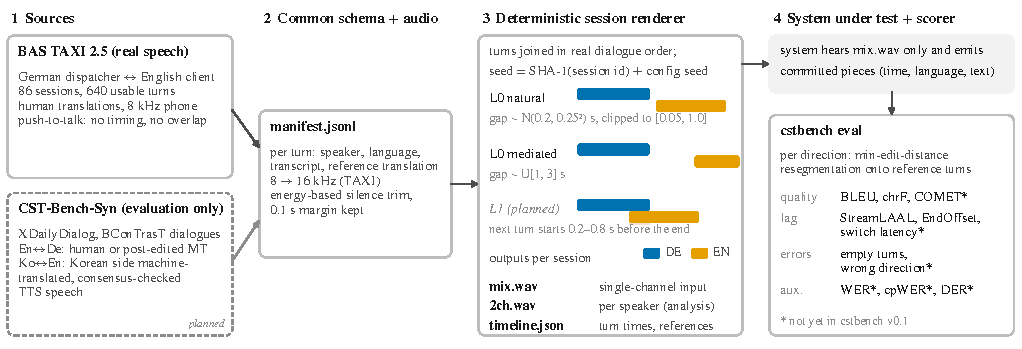
\includegraphics[width=\textwidth]{figures/fig2_benchmark.pdf}
  \caption{The \bench pipeline (planned parts dashed or starred). For TAXI, we release only code, checksums and per-turn scores.}
  \label{fig:bench}
\end{figure*}

\bench renders two-language dialogues as continuous mono sessions that differ only in turn-taking, and scores what a system commits, and when (\cref{fig:bench,tab:bench}). It serves evaluation only; nothing is tuned on \taxi.

% =====================================================================
% Table 2 (tab:bench): CST-Bench composition. Single column; included
% from Sec. 4.2. TAXI L0 values are measured on the cstbench v0.1.0
% build of BAS TAXI 2.5. TAXI L1 and the synthetic track are planned:
% their condition-specific cells use \tbd (plan targets are not facts).
% Measured natural width: 257.9pt at \footnotesize (9pt in ICML), 233.1pt at 8pt (column 234.9pt).
% =====================================================================
\begin{table}[t]
  \caption{\bench composition (TAXI: \taxi; Syn: \syn). TAXI speech, content and turn order are real; its timing is synthetic. The TAXI conditions render the same turns, so merged cells hold for all three. Pairs are \dir{De}{En}\,/\,\dir{En}{De} (German\,/\,English source turns). Speech is counted after silence trimming. Turns/session: median (mean; range); switches: total (median per session). Gaps are taken at speaker changes; occupancy is the share of session time covered by turns. $^\ast$Planned; blank cells are pending. $^\ddagger$English side human, Korean side machine-translated and consensus-checked.}
  \label{tab:bench}
  \centering
  \fontsize{8}{9.5}\selectfont % 8pt (ICML \footnotesize is 9pt): fits the width
  \setlength{\tabcolsep}{3pt}
  \begin{tabular}{@{}lccccc@{}}
    \toprule
    & \multicolumn{3}{c}{TAXI (real speech)} & \multicolumn{2}{c}{Syn (TTS)$^\ast$} \\
    \cmidrule(lr){2-4}\cmidrule(l){5-6}
    & \makecell{L0\\natural} & \makecell{L0\\mediated} & \makecell{L1 turn-end\\overlap$^\ast$} & \pair{En}{De} & \pair{Ko}{En} \\
    \midrule
    Source speech      & \multicolumn{3}{c}{telephone, 8$\to$16\,kHz}     & TTS   & TTS              \\
    References         & \multicolumn{3}{c}{human}                         & human & mixed$^\ddagger$ \\
    Sessions           & \multicolumn{3}{c}{86}                            & \tbd  & \tbd             \\
    Usable turns       & \multicolumn{3}{c}{640 (349\,/\,291)}             & \tbd  & \tbd             \\
    Speech (min)       & \multicolumn{3}{c}{40.378 (17.953\,/\,22.425)}    & \tbd  & \tbd             \\
    Source words       & \multicolumn{3}{c}{6,815 (3,228\,/\,3,587)}       & \tbd  & \tbd             \\
    Reference words    & \multicolumn{3}{c}{6,617 (3,339\,/\,3,278)}       & \tbd  & \tbd             \\
    Mean turn (s)      & \multicolumn{3}{c}{3.086\,/\,4.624}               & \tbd  & \tbd             \\
    Turns/session      & \multicolumn{3}{c}{7 (7.44; 1--17)}               & \tbd  & \tbd             \\
    Switches           & \multicolumn{3}{c}{540 (6)}                       & \tbd  & \tbd             \\
    \midrule
    Session audio (h)  & 0.737  & 0.998  & \tbd & \tbd & \tbd \\
    Median session (s) & 29.023 & 39.316 & \tbd & \tbd & \tbd \\
    Gap mean (s)       & 0.257  & 1.995  & \tbd & \tbd & \tbd \\
    Gap median (s)     & 0.223  & 2.026  & \tbd & \tbd & \tbd \\
    Overlap ratio      & 0.0    & 0.0    & \tbd & \tbd & \tbd \\
    Occupancy (\%)     & 91.27  & 67.42  & \tbd & \tbd & \tbd \\
    \bottomrule
  \end{tabular}
\end{table}


\paragraph{Real track: \taxi.}\label{sec:bench-taxi}
TAXI~2.5 holds telephone dialogues between German-speaking taxi dispatchers and English-speaking clients, with human translations of both sides \citep{bas2001taxi,reichel2016bas}. Push-to-talk recording left one file per turn, without timing or overlap, so in \taxi only the timing is synthetic, and the mono mix of its 640 usable turns simulates a shared device, not the original calls (\cref{app:taxi}). Language coincides with role, and the German dispatcher opens 85 of 86 sessions.

\paragraph{Synthetic track: \syn.}\label{sec:bench-syn}
\draftnote{planned: nothing in this track is built yet}
Voiced by TTS, it cannot replace a real test set but adds overlap measurable at the word level, a distant pair (\pair{Ko}{En}) and both speaker--language assignments, so that language predicts neither role nor first direction. Speakers take turns from two language versions of one XDailyDialog \citep{liu2023xdailydialog} or BConTrasT \citep{farajian2020findings} dialogue, each supplying the other's references; Korean text is consensus-filtered machine translation (\cref{app:syn}).

\paragraph{Timing conditions.}\label{sec:bench-timing}
Turns keep their dialogue order, with within-speaker pauses from $\mathcal{U}[0.3,0.8]$\,s and per-session seeds (\cref{app:taxi}). At speaker changes, \emph{L0 natural} draws gaps from $\mathcal{N}(0.2,0.25^2)$\,s clipped to $[0.05,1]$\,s, around the typical 200\,ms gap, and \emph{L0 mediated} from $\mathcal{U}[1,3]$\,s, as when listeners first read the translation; as gaps separate turn intervals that keep 0.1\,s margins, silences between speech are up to 0.2\,s longer. \emph{L1} starts each new speaker's turn $\mathcal{U}[0.2,0.8]$\,s before the previous one ends, adding overlap to real speech. Per-speaker channels serve an oracle-separation diagnostic.
\draftnote{planned: L1, with a cap for short turns fixed before any baseline run, and word-level overlap; decision needed: whether the L1 overlap is measured between energetic frames or between margin-inclusive intervals, which leaves up to 0.2\,s less overlapping speech}

% Fig. 3 (fig:model) belongs to Sec. 5 but is defined here, so that it floats
% to the top of the page where Sec. 5 starts (a figure* appears at the earliest
% on the page after its definition). Edit its caption here.
\begin{figure*}[t]
  \centering
  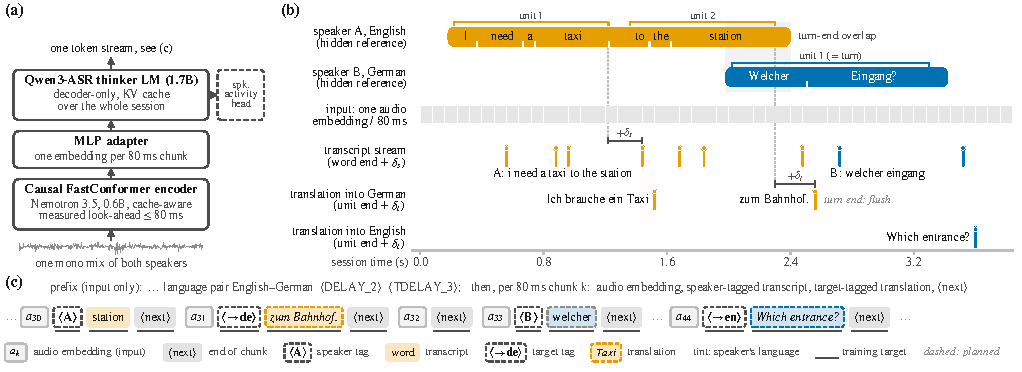
\includegraphics[width=\textwidth]{figures/fig3_model.pdf}
  \caption{\model and conversational delayed streams (illustrative timings; $\delta_s=2$, $\delta_t=3$).
    (a)~Architecture.
    (b)~Targets: a transcript word is due $\delta_s$ chunks, the translation of a verified meaning unit $\delta_t$ chunks, after the chunk in which it ends; a turn end forces a commit.
    (c)~The resulting token stream. Dashed: planned.
    \protect\draftnote{built today: the encoder--adapter--LM backbone, trained for single-speaker English and Korean transcription}}
  \label{fig:model}
\end{figure*}

\paragraph{Scoring.}\label{sec:bench-scoring}
\scorer resegments the committed words of each session and output language onto the references of that direction by word-level Levenshtein alignment \citep{matusov2005evaluating}, keeping each word's emission time, and reports COMET \citep{rei2022comet}, chrF \citep{popovic2015chrf} and BLEU \citep{papineni2002bleu} per direction on lowercased, unpunctuated text (\cref{app:scorer}). For turn $n$, with $L_n=e_n-b_n$ and words $j=1,\dots,|h_n|$ resegmented to it and emitted at $t_{n,j}$, let $d_{n,j}=\max(0,t_{n,j}-b_n)$ and $\rho_n=L_n/\max(|h_n|,|r_n|)$. Then
\begin{align}
  \mathrm{StreamLAAL}_n &= \tfrac{1}{J_n}\textstyle\sum_{j=1}^{J_n}\bigl(d_{n,j}-(j-1)\,\rho_n\bigr), \label{eq:bench-laal}\\
  \mathrm{EndOffset}_n &= t_{n,|h_n|}-e_n, \label{eq:bench-endoffset}\\
  \mathrm{SwitchLatency}_n &= d_{n,1} \quad\text{for } n>1,\ s_n\neq s_{n-1}, \label{eq:bench-switch}
\end{align}
where $J_n$ is the first $j$ with $d_{n,j}\ge L_n$ (else $|h_n|$). \Cref{eq:bench-laal} is length-adaptive Average Lagging (LAAL; \citealp{ma2019stacl,papi2022overgeneration}) on resegmented turns, i.e., \laal \citep{papi2024streamatt}: the lag \emph{within} a turn, $L_n$ for output committed at turn ends. As \laal ignores words after $J_n$, \eo, SimulEval's EndOffset taken per turn \citep{ma2020simuleval,seamless2023seamless}, measures the wait after the speaker stops; switch latency is the matching StartOffset at direction changes. A committed piece is \emph{wrong-direction} if turns are open but none is translated into its language, if a text language identifier assigns it to the other language, or if it copies an open turn's transcript; we report the share of committed words in such pieces. Transcripts are scored by WER and cpWER (\citealp{watanabe2020chime}; for Korean, cpCER on characters), speakers by DER.

\paragraph{Statistics and validation.}
Comparisons carry 95\% confidence intervals (CIs) from a session-clustered paired bootstrap \citep{koehn2004statistical}; main comparisons, fixed before the test runs, are Holm-corrected (\citealp{holm1979simple}; \cref{app:repro}). Controlled perturbations of the reference output test whether BLEU, chrF, \laal, \eo and wrong-direction words move only as expected (\cref{tab:sanity}). Copying the source lowered \deen \laal below that of the reference committed at turn ends (\prelim{2.276} vs.\ \prelim{3.086}\,s; $^\dagger$preliminary), so \cref{tab:main} shows latency next to quality and empty turns, and \cref{app:scorer} defines a matched-word latency.
\draftnote{scorer v0.1 computes BLEU, chrF, \laal, \eo, empty turns and wrong-language words given gold turn IDs; the other metrics (including the length ratio and the matched-word latency), the bootstrap and a pinned number normaliser are being added; rows 3--10 of \cref{tab:sanity} are planned}

% !TEX root = ../main.tex
% ---------------------------------------------------------------------------
% Section 5: the unified model (conversational delayed streams).
% Built: the streaming ASR backbone (Sec. 5.1). Planned: Secs. 5.2-5.4; every
% planned part carries a \draftnote.
% Budget: <= 620 words of prose (wordcount.py) + Fig. 3, about 1.1 pages.
% Moved to App. F (app:model): encoder and thinker specifications, the loss
% weights, delay medians, backbone WERs, the [56,3] trade-off, Stage-0/1 and
% Stage-2/3 data recipes, per-speaker forced alignment before mixing, the
% decoding procedure and cap, the session length in audio positions,
% licences, EXAONE exclusion, the real-time context (also in Sec. 7).
% Moved to App. G (app:units): minimum-unit sizes, pilot LAAL/chrF values,
% collapse counts, the TAXI turn-length comparison.
% Stated once elsewhere, not repeated here: that the baselines, unlike the
% model and the M1-based controls, never see simulated sessions (Sec. 6.6,
% App. F); the decoupled twin (Sec. 6.6, App. D, App. F); that the output
% language fixes the direction (Def. 1). Coupling claims are left to the
% decoupled twin and the same-backbone cascade (Sec. 6.6).
% Within a turn only verified units are committed; a turn end commits the
% rest, so the novelty sentence says "commit units verified ...", not "only".
% Floats: Fig. 3 (figure*, fig:model), defined in sections/04_bench.tex so
% that it lands on the page where this section starts. One sentence per line.
% Labels kept: sec:model, sec:model-backbone, sec:model-stream,
% sec:model-targets and sec:model-inference (both on Sec. 5.3, which now
% holds the latency accounting), sec:model-training, eq:chunk, eq:loss.
% eq:delay was only referenced here; the delay rule is now inline.
% ---------------------------------------------------------------------------
% Special tokens of the serialized stream, e.g. \mdltok{next}, \mdltok{A}, \mdltok{{\to}de}.
% Robust, so it also works in captions; later files may reuse it.
\DeclareRobustCommand{\mdltok}[1]{\ensuremath{\langle\mathrm{#1}\rangle}}

\section{\model: Conversational Delayed Streams}\label{sec:model}

% Fig. 3 (figure*, fig:model) is defined in sections/04_bench.tex, before
% \paragraph{Scoring.}: a figure* appears at the earliest on the page after its
% definition, so defining it here would push it one page past this section.

After each $\Delta=80$\,ms audio chunk, the causal speech LLM \model writes zero or more tokens of a speaker-tagged transcript and translations into both languages (\cref{fig:model}): reading and writing become next-token prediction.
Unlike delayed streams modeling (one delayed text stream; \citealp{zeghidour2025streaming}), \emph{conversational delayed streams} delay each channel separately; unlike Hibiki's alignment-based per-word delays \citep{labiausse2025highfidelity}, they commit units verified by translating the source heard so far.
\draftnote{planned: only the backbone of \cref{sec:model-backbone} is built; \cref{sec:model-stream,sec:model-targets,sec:model-training} describe the design, and no \task result exists yet}

\subsection{Streaming backbone}\label{sec:model-backbone}
A cache-aware FastConformer encoder from Nemotron~3.5 ASR Streaming 0.6B \citep{nvidia2026nemotron35asr}, with a measured look-ahead of at most 80\,ms, feeds one embedding $a_k$ per chunk $k$, via an MLP adapter, to the 1.7B Qwen3-ASR language model, the \emph{thinker} \citep{shi2026qwen3asr}, replacing its non-causal audio encoder (\cref{app:model}).
After a prefix with the language and a delay token \mdltok{DELAY\_\delta}, each chunk holds $a_k$, the text tokens due in it and an end-of-chunk token \mdltok{next}; a word ending at $t$ is due in chunk $\lfloor t/\Delta\rfloor+\delta$.

\subsection{One serialized stream}\label{sec:model-stream}
The prefix names the language pair and two delays, $\delta_s$ for transcripts and $\delta_t$ for translations, sampled per training session.
Chunk $k$ reads
\begin{equation}\label{eq:chunk}
  B_k = a_k\,\mdltok{\hat s_1}\,z_1\cdots\mdltok{{\to}\lambda_1}\,y_1\cdots\mdltok{next},
\end{equation}
where $z_j$ are words of speaker $\hat s_j\in\{\mathrm{A},\mathrm{B}\}$, numbered by arrival, and $y_i$ translates one unit into language $\lambda_i$.
Each tagged segment is a committed piece (\cref{def:cst}), making the speaker and direction state explicit; under overlap, words are ordered by end time, as in t-SOT \citep{kanda2022streaming} and JSTAR \citep{moritz2025transcribing}.
We minimise
\begin{equation}\label{eq:loss}
  \mathcal{L}=-\textstyle\sum_{m\in\mathcal{Y}}w_m\log p_\theta(o_m\mid o_{<m})\,\big/\sum_{m\in\mathcal{Y}}w_m
\end{equation}
over the labelled positions $\mathcal{Y}$ (text, tags, \mdltok{next}) of the tokens $o$, with $w_m<1$ only for \mdltok{next} (\cref{app:model}); a two-slot, arrival-order activity head \citep{park2025sortformer} adds a binary cross-entropy and serves DER.
The session-long KV cache lets both sides condition every decision.
\draftnote{planned: the two speaker tags are reserved in the vocabulary but untrained; translation segments, the translation delay token and the activity head do not exist yet}

\subsection{Commit targets and latency}\label{sec:model-targets}\label{sec:model-inference}
A teacher LLM (Qwen3.8-27B) translates each source turn $u_{1:I}$ into $v$, and contextual alignment \citep{labiausse2025highfidelity} maps target word $v_j$ to $\alpha_j=\arg\max_i\,[\phi_j(i)-\phi_j(i-1)]$, $\phi_j(i)$ being its log-probability when $v$ is force-decoded from $u_{1:i}$.
Position $i$ is a candidate if $\{j:\alpha_j\le i\}=\{1,\dots,\kappa\}$ with $\kappa$ above the committed length, as meaning units require \citep{zhang2020learning}, and the source has grown by a minimum unit.
A candidate becomes a verified meaning unit (MU2) if the teacher's translation of the new source, given the committed text, is in the target language and reaches chrF${}\ge50$ against the newly aligned span of $v$.
Its translation is due $\delta_t\ge\delta_s$ chunks after its source's last chunk; a turn end commits the rest of the turn, so \model must detect it.
Relative to the teacher's alignment, targets thus never anticipate unheard speech, whereas sentence-level targets \citep{ma2019stacl} require anticipating clause-final German and Korean verbs; but commit points depend on the whole turn, so \model imitates a privileged teacher.
In a text-level \pair{Ko}{En} pilot (silver references; utterances much longer than \taxi turns), MU2 roughly halves the lag of utterance-end commits (a LAAL variant), losing at most 2.2 chrF (\cref{app:units}).
\draftnote{planned: MU2 targets for \pair{En}{De} and at training scale; the German minimum unit and the $\delta_t$ values are set on held-out data}

A token written after chunk $k$ is time-stamped $(k+1)\Delta+\ell_{\mathrm{enc}}+c$, so on schedule its latency after evidence ending at $t$ is $q+\delta\Delta+\ell_{\mathrm{enc}}+c$: quantisation $q\in(0,\Delta]$, stream delay $\delta\in\{\delta_s,\delta_t\}$, encoder look-ahead $\ell_{\mathrm{enc}}$ (80\,ms) and compute time $c$ (zero on the ideal clock; \cref{tab:ca-latency}).
As turn ends force commits, \eo then stays near $q+\delta_t\Delta+\ell_{\mathrm{enc}}+c$.

\subsection{Training without real cross-lingual conversations}\label{sec:model-training}
After single-speaker English and Korean ASR training (Stages~0--1), Stage~2 trains M1 for speaker-attributed transcription on simulated sessions with gaps and overlaps drawn more broadly than the benchmark's; Stage~3 adds translations committed at turn ends (M2) or at MU2 (M3) (\cref{tab:training}).
Training excludes \taxi and \syn dialogues and voices (\cref{app:model}).
\draftnote{planned: Stages 2--3; German training data has yet to be obtained}

% =====================================================================
% Section 6: Experiments (sec:exp).
% Floats, in numbering order: Table 3 (tables/tab_main.tex, table*),
% Fig. 4 (fig:ql, single column, Sec. 6.2), Fig. 5 (fig:gap, figure*,
% defined at the start of Sec. 6.3 so that it lands near Sec. 6.4),
% Table 4 (tables/tab_factorial.tex) and Table 5 (tables/tab_aux.tex),
% both input in Sec. 6.3 so that Table 5 is not pushed past Sec. 7,
% and Table 6 (tables/tab_ablation.tex).
% Measured so far (preliminary, \prelim): the offline rows of Table 3 and
% the two ASR WERs of Table 5. Everything else is pending: the result
% paragraphs are templates with \tbdtext; do not add findings before the
% runs exist.
% Wording: the offline systems and Gold->LLM (MU2) get oracle input but are
% not called bounds (no dialogue history; Whisper ST already passes
% Gold->LLM on De->En BLEU). R and Fig. 5 use one pipeline under both
% wrappers, that of Table 4.
% =====================================================================
\section{Experiments}\label{sec:exp}

% =====================================================================
% Table 3 (tab:main): main results on CST-Bench-TAXI, L0 natural timing,
% ideal clock (table*, 8pt; 529pt wide at 9pt, 480pt at 8pt). Included at the start of Sec. 6.
% Measured so far (preliminary, \prelim): BLEU, chrF and StreamLAAL of the
% three offline rows; their EndOffset is 0 by construction on the ideal
% clock. They were scored with gold turn IDs (scorer oracle mode, no
% resegmentation); the caption says so. Every other cell is pending
% (\tbd = blank); -- marks a direction the system does not cover, and the
% pooled columns of single-direction systems. Systems are defined in Sec. 6.1
% (sec:exp-setup); names follow Table A5 (tab:conditions), and the caption
% of Fig. 4 (fig:ql) maps its legend labels to them.
% =====================================================================
\begin{table*}[t]
  \caption{Real dialogues: \taxi, L0 natural timing, ideal clock. Rows: upper bounds with oracle input, the consecutive cascade, streaming systems and \model (\cref{sec:exp-setup}; LLM: Qwen3.8-27B), each at its main operating point; \model M2 commits translations at turn ends, and M3 at MU2 units with a low or a high $\delta_t$. Seg.: oracle = gold turns and source language; realistic = VAD and language-ID routing; none = the system segments the stream itself. Per direction: mean \laal and median \eo in seconds; the last three columns pool both directions (switch latency: median, in seconds) and do not apply to single-direction systems, which cannot be the best pipeline (\cref{tab:factorial,fig:gap}). \Cref{tab:conditions} gives 95\% session-bootstrap CIs for the rows it repeats, except for BLEU. Blank: pending; --: direction not covered. $^\dagger$preliminary and scored by gold turn ID (oracle mode of \cref{app:scorer}), not resegmented; to be re-run under the final protocol. $^\ddagger$0 by construction: the output is emitted at the oracle turn end.}
  \label{tab:main}
  \centering
  \fontsize{8}{9.5}\selectfont % 8pt (ICML \footnotesize is 9pt): fits the width
  \setlength{\tabcolsep}{2.5pt}
  \begin{tabular}{@{}ll*{13}{c}@{}}
    \toprule
    & & \multicolumn{5}{c}{\ende} & \multicolumn{5}{c}{\deen} & \multicolumn{3}{c}{Both directions} \\
    \cmidrule(lr){3-7}\cmidrule(lr){8-12}\cmidrule(l){13-15}
    System & Seg.
      & COMET & BLEU & chrF & \makecell[b]{Stream-\\LAAL} & \makecell[b]{End-\\Offset}
      & COMET & BLEU & chrF & \makecell[b]{Stream-\\LAAL} & \makecell[b]{End-\\Offset}
      & \makecell[b]{Wrong\\dir.\ (\%)} & \makecell[b]{Switch\\latency} & \makecell[b]{Empty\\turns (\%)} \\
    \midrule
    Gold$\to$LLM & oracle
      & \tbd & \prelim{48.31} & \prelim{71.72} & \prelim{4.62} & $0^{\ddagger}$
      & \tbd & \prelim{30.60} & \prelim{58.05} & \prelim{3.09} & $0^{\ddagger}$
      & \tbd & \tbd & \tbd \\
    ASR$\to$LLM & oracle
      & \tbd & \prelim{42.66} & \prelim{67.97} & \prelim{4.62} & $0^{\ddagger}$
      & \tbd & \prelim{28.11} & \prelim{56.61} & \prelim{3.09} & $0^{\ddagger}$
      & \tbd & \tbd & \tbd \\
    Whisper ST & oracle
      & --   & --   & --   & --   & --
      & \tbd & \prelim{30.69} & \prelim{56.67} & \prelim{3.09} & $0^{\ddagger}$
      & --   & --   & --   \\
    Gold$\to$LLM (MU2) & oracle
      & \tbd & \tbd & \tbd & \tbd & \tbd
      & \tbd & \tbd & \tbd & \tbd & \tbd
      & \tbd & \tbd & \tbd \\
    \midrule
    Consecutive cascade & realistic
      & \tbd & \tbd & \tbd & \tbd & \tbd
      & \tbd & \tbd & \tbd & \tbd & \tbd
      & \tbd & \tbd & \tbd \\
    \midrule
    \multirow{2}{*}{SeamlessStreaming} & oracle
      & \tbd & \tbd & \tbd & \tbd & \tbd
      & \tbd & \tbd & \tbd & \tbd & \tbd
      & \tbd & \tbd & \tbd \\
      & realistic
      & \tbd & \tbd & \tbd & \tbd & \tbd
      & \tbd & \tbd & \tbd & \tbd & \tbd
      & \tbd & \tbd & \tbd \\
    2$\times$SeamlessStreaming & none
      & \tbd & \tbd & \tbd & \tbd & \tbd
      & \tbd & \tbd & \tbd & \tbd & \tbd
      & \tbd & \tbd & \tbd \\
    \multirow{2}{*}{Streaming cascade} & oracle
      & \tbd & \tbd & \tbd & \tbd & \tbd
      & \tbd & \tbd & \tbd & \tbd & \tbd
      & \tbd & \tbd & \tbd \\
      & realistic
      & \tbd & \tbd & \tbd & \tbd & \tbd
      & \tbd & \tbd & \tbd & \tbd & \tbd
      & \tbd & \tbd & \tbd \\
    \multirow{2}{*}{M4T v2 + AlignAtt} & oracle
      & \tbd & \tbd & \tbd & \tbd & \tbd
      & \tbd & \tbd & \tbd & \tbd & \tbd
      & \tbd & \tbd & \tbd \\
      & realistic
      & \tbd & \tbd & \tbd & \tbd & \tbd
      & \tbd & \tbd & \tbd & \tbd & \tbd
      & \tbd & \tbd & \tbd \\
    \multirow{2}{*}{StreamSpeech} & oracle
      & --   & --   & --   & --   & --
      & \tbd & \tbd & \tbd & \tbd & \tbd
      & --   & --   & --   \\
      & realistic
      & --   & --   & --   & --   & --
      & \tbd & \tbd & \tbd & \tbd & \tbd
      & --   & --   & --   \\
    \multirow{2}{*}{InfiniSST} & oracle
      & \tbd & \tbd & \tbd & \tbd & \tbd
      & --   & --   & --   & --   & --
      & --   & --   & --   \\
      & realistic
      & \tbd & \tbd & \tbd & \tbd & \tbd
      & --   & --   & --   & --   & --
      & --   & --   & --   \\
    \midrule
    \model M2 & none
      & \tbd & \tbd & \tbd & \tbd & \tbd
      & \tbd & \tbd & \tbd & \tbd & \tbd
      & \tbd & \tbd & \tbd \\
    \model M3, low $\delta_t$ & none
      & \tbd & \tbd & \tbd & \tbd & \tbd
      & \tbd & \tbd & \tbd & \tbd & \tbd
      & \tbd & \tbd & \tbd \\
    \model M3, high $\delta_t$ & none
      & \tbd & \tbd & \tbd & \tbd & \tbd
      & \tbd & \tbd & \tbd & \tbd & \tbd
      & \tbd & \tbd & \tbd \\
    \bottomrule
  \end{tabular}
\end{table*}


We answer RQ1--RQ4 (\cref{sec:intro}) on real dialogues first; synthetic sessions add the distant pair and a check against real rankings. Every comparison carries a session-clustered 95\% confidence interval (CI; \cref{app:repro}), and we do not interpret differences inside it.
\draftnote{planned: apart from the preliminary offline rows of \cref{tab:main} and ASR WERs of \cref{tab:aux}, no experiment of this section has been run}

\subsection{Setup}\label{sec:exp-setup}

\paragraph{Systems.}
Every system receives the session's language pair.
Offline systems cut each oracle turn from the mix and translate it after the turn ends, one turn per prompt and without dialogue history: Qwen3.8-27B (``LLM'') translates the gold transcript (Gold$\to$LLM) or the transcript of Qwen3-ASR-1.7B, given the language \citep[ASR$\to$LLM;][]{shi2026qwen3asr}, and Whisper-large-v3 translates speech into English \citep[Whisper ST;][]{radford2023robust}.
Gold$\to$LLM (MU2) is a streaming variant with oracle input: the LLM reads gold transcripts at forced-aligned word times and commits at the verified meaning units (MU2) of \cref{sec:model}, whose boundaries are found with the whole turn in view (non-causal).
The consecutive cascade detects turn ends with the realistic wrapper described below, then transcribes and translates each segment like ASR$\to$LLM.
The streaming systems are SeamlessStreaming \citep{seamless2023seamless}, StreamSpeech \citep{zhang2024streamspeech} (\deen only), InfiniSST \citep{ouyang2025infinisst} (\ende only) and two systems that run offline translation models with a streaming policy.
In the streaming cascade, the LLM re-translates the growing transcript of the Nemotron~3.5 streaming RNN-T \citep{nvidia2026nemotron35asr} and commits the prefix on which two consecutive outputs agree (LocalAgreement-2, LA-2; \citealp{liu2020lowlatency,polak2022cuni,machacek2023turning}).
M4T v2 + AlignAtt runs SeamlessM4T~v2 \citep{seamless2025joint,seamless2023seamless} with the AlignAtt policy \citep{papi2023alignatt} in simulstream \citep{gaido2025simulstream}.
As a naive bidirectional baseline, 2$\times$SeamlessStreaming runs one instance per target language on the whole mix, without routing.
\model runs as M2, which commits translations at turn ends, and as M3, which commits at MU2 units and runs at a low and a high $\delta_t$ (\cref{sec:model}).
\Cref{tab:baselines} lists checkpoints, sizes and licences.
\draftnote{InfiniSST only if its weights are released; Canary-1B-v2 \citep{sekoyan2025canary} with AlignAtt is optional; Hibiki-Zero (\deen; public weights) is not yet in the plan}

\paragraph{Wrappers and operating points.}
A system that translates one direction runs as one instance per target language behind a wrapper; we call the combination a pipeline (\cref{app:baselines}).
The oracle wrapper cuts gold turns from the mix and routes each by its gold source language.
The realistic wrapper segments the stream with Silero VAD \citep{silero2024silero} and routes each segment by spoken language identification restricted to the pair, decided at the segment start and re-routed if the decision flips.
Baselines are not fine-tuned.
Each streaming system has two operating points, one of them its main point, chosen once on the \syn calibration split by a rule fixed before any test run.
\draftnote{until \syn exists, documented defaults stand in for calibrated operating points; which of the two latency budgets gives the main point is still to be fixed}

\paragraph{Metrics and statistics.}
Per direction, we report COMET, chrF and BLEU, \laal (lag within a turn) and median \eo (the listener's wait after a turn); pooled over directions, we report wrong-direction words, median switch latency and empty turns (\cref{sec:bench}).
We rank systems by COMET rather than BLEU \citep{kocmi2021ship}; on \taxi, whose references are lowercase and unpunctuated, chrF takes its place if the two rank systems differently (\cref{sec:exp-validity}).
Latency uses the ideal clock; computation-aware latency, measured for one unbatched stream on one GPU type, is in \cref{tab:ca-latency}.
The oracle-gap recovery of \model is $R=(Q_{\mathrm{ours}}-Q_{\mathrm{real}})/(Q_{\mathrm{oracle}}-Q_{\mathrm{real}})$, where $Q$ is COMET: of \model, and of the pipeline of \cref{tab:factorial} under the oracle and the realistic wrapper; $R$ comes with a bootstrap CI and is reported only where the CI of the gap excludes 0.
Daggers mark preliminary numbers, to be re-run under the final protocol.

\subsection{Real dialogues (RQ1, RQ3)}\label{sec:exp-real}

\begin{figure}[t]
  \centering
  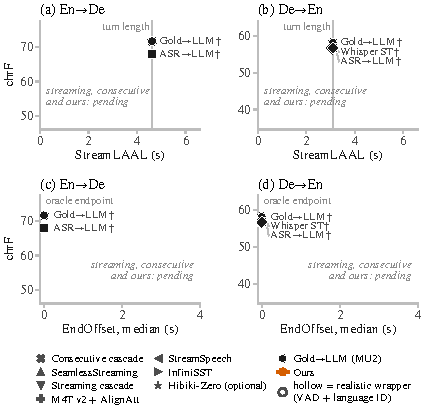
\includegraphics[width=0.89\columnwidth]{figures/fig4_quality_latency.pdf}
  \caption{Quality vs.\ latency on \taxi (L0 natural, ideal clock), per direction: chrF against \laal (a, b) and against median \eo (c, d). Black outlines mark systems with oracle input, although drawn hollow; by construction, the labelled offline systems sit at the mean source-turn duration on \laal (`turn length') and at 0 on \eo (`oracle endpoint'). The other systems are pending: filled markers will show oracle segmentation and hollow markers VAD and language-ID routing, with grey arrows joining the two for each system, and a vermillion curve will trace \model over its $\delta_t$ operating points. Legend: Seamless = SeamlessStreaming, Cascade-LA = streaming cascade, M4Tv2-AA = M4T v2 + AlignAtt, Ours = \model. chrF stands in until COMET is in the scorer. $^\dagger$preliminary; to be re-run under the final protocol.}
  \label{fig:ql}
\end{figure}

\Cref{tab:main} and \cref{fig:ql} compare all systems on \taxi under L0 natural timing.
Given oracle turns, Gold$\to$LLM reaches \prelim{48.31} BLEU and \prelim{71.72} chrF for \ende, and \prelim{30.60} and \prelim{58.05} for \deen.
ASR transcripts cost \prelim{5.65} and \prelim{2.49} BLEU, in line with the higher WER of Qwen3-ASR-1.7B on English than on German turns (\prelim{13.78}\% vs.\ \prelim{7.33}\%; \cref{tab:aux}), and Whisper ST reaches \prelim{30.69} BLEU into English.
These offline systems look instantaneous on \eo, at most about \prelim{0.2}\,s even with measured, batched computation (\cref{tab:ca-latency}), only because they receive oracle endpoints.
The consecutive cascade, which must detect endpoints, makes listeners wait a median of \tbdtext{}\,s at \tbdtext{} COMET.
Realistic segmentation costs the streaming systems \tbdtext{} COMET (arrows in \cref{fig:ql}), and \model reaches \tbdtext{} COMET at a median \eo of \tbdtext{}\,s without oracle input.

\subsection{Where pipelines fail (RQ1)}\label{sec:exp-fail}

% Fig. 5 is discussed in Sec. 6.4; it is defined here so that the full-width
% float can reach the top of the page that holds Sec. 6.4.
\begin{figure*}[t]
  \centering
  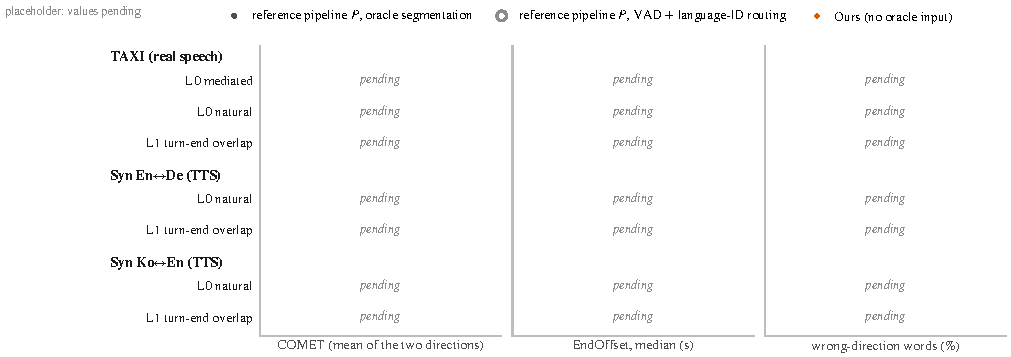
\includegraphics[width=\textwidth]{figures/fig5_oracle_gap.pdf}
  \caption{Where the conversational difficulty lies (values pending; numbers will be in \cref{tab:conditions}). For each timing condition and language pair: the best pipeline with oracle turn segmentation (filled) and with VAD and language-ID routing (hollow), and \model (diamond; no oracle input). One pipeline serves every row and both wrappers: that of \cref{tab:factorial}, with the highest realistic-wrapper COMET on \taxi L0 natural among pipelines that cover both directions, at its main operating point. Panels: COMET (mean of the two directions), median \eo and wrong-direction words.}
  \label{fig:gap}
\end{figure*}

% Table 5 (tab:aux) is input here, right after Table 4, so that it can
% share a page with Table 4 instead of floating past Sec. 7.
% =====================================================================
% Table 4 (tab:factorial): oracle-component factorial for the reference
% pipeline P of Sec. 6.1 on CST-Bench-TAXI, ideal clock (single column,
% 8pt). Included in Sec. 6.3.
% No values yet: every cell is pending (\tbd = blank); -- marks cells that
% do not apply. Language-ID routing accuracy is reported in the text; the
% factor effects E_T, E_L and their interaction, with their CIs, are
% defined in App. E, and the same factorial for the second-best pipeline
% goes to App. E. Cells carry no CIs; the caption points to App. E, not to
% tab:conditions, which has neither rows 2, 3, 5 nor the direction mean.
% How a VAD segment gets its gold language (the most-overlapping turn) is
% stated in App. D (app:baselines), not in the caption.
% =====================================================================
\begin{table}[t]
  \caption{Oracle-component factorial for the reference pipeline $P$ (\cref{sec:exp-setup}) on \taxi, ideal clock; factor effects with CIs: \cref{app:results}. \cmark: oracle T (gold turns, else VAD), L (gold language, else language ID; \cref{app:baselines}) or S (two-channel separation; L1 only). Row~4 is realistic. COMET: mean of both directions; $\Delta$COMET: L1 COMET minus row~1's L1 COMET.}
  \label{tab:factorial}
  \centering
  \fontsize{8}{9.5}\selectfont % 8pt (ICML \footnotesize is 9pt): fits the width
  \setlength{\tabcolsep}{2pt}
  \begin{tabular}{@{}cccccccccc@{}}
    \toprule
    & \multicolumn{3}{c}{Oracle} & \multicolumn{2}{c}{L0 natural} & \multicolumn{4}{c}{L1 turn-end overlap} \\
    \cmidrule(lr){2-4}\cmidrule(lr){5-6}\cmidrule(l){7-10}
    \# & T & L & S
      & COMET & \makecell[b]{Wrong\\dir.\ (\%)}
      & COMET & \makecell[b]{Wrong\\dir.\ (\%)} & \makecell[b]{Switch\\latency} & $\Delta$COMET \\
    \midrule
    1 & \cmark & \cmark & \xmark & \tbd & \tbd & \tbd & \tbd & \tbd & --   \\
    2 & \cmark & \xmark & \xmark & \tbd & \tbd & \tbd & \tbd & \tbd & \tbd \\
    3 & \xmark & \cmark & \xmark & \tbd & \tbd & \tbd & \tbd & \tbd & \tbd \\
    4 & \xmark & \xmark & \xmark & \tbd & \tbd & \tbd & \tbd & \tbd & \tbd \\
    5 & \cmark & \cmark & \cmark & --   & --   & \tbd & \tbd & \tbd & \tbd \\
    \midrule
    \multicolumn{4}{@{}l}{6\enspace\model} & \tbd & \tbd & \tbd & \tbd & \tbd & \tbd \\
    \bottomrule
  \end{tabular}
\end{table}

% =====================================================================
% Table 5 (tab:aux): transcription and two-speaker attribution
% (single column, \footnotesize). Included in Sec. 6.3, discussed in 6.5.
% Layout: systems as columns, set x metric as rows (fits one column; about
% 232pt in a 234.9pt column, so no eighth column fits).
% Measured so far (preliminary, \prelim): the two TAXI WERs of Qwen3-ASR-1.7B
% on oracle turns. Every other cell is pending (\tbd = blank); -- marks
% cells that do not apply (oracle speakers, offline output). The diarization
% baselines are called "diar." here so that they are not confused with the
% translation "streaming cascade" of Table 3. Context delays of the earlier
% single-speaker 0.6B backbones are in App. F, not here; tcpWER and DER
% without a collar are in App. E.
% =====================================================================
\begin{table}[t]
  \caption{Who said what: error rates (\%); systems: \cref{sec:exp-aux}. L0: L0 natural; Syn: \syn \pair{Ko}{En}. DER: 0.25\,s collar. Delay: median delay of transcript words. --: not applicable. $^\dagger$Preliminary.}
  \label{tab:aux}
  \centering
  \footnotesize
  \setlength{\tabcolsep}{2.6pt}
  \begin{tabular}{@{}llccccc@{}}
    \toprule
    & & & & & \multicolumn{2}{c}{\model} \\
    \cmidrule(l){6-7}
    Set & Metric & \makecell[b]{Oracle\\ASR} & \makecell[b]{Offline\\diar.} & \makecell[b]{Streaming\\diar.} & $\delta_s{=}2$ & $\delta_s{=}4$ \\
    \midrule
    \multirow{5}{*}{TAXI L0} & WER En     & \prelim{13.78} & \tbd & \tbd & \tbd & \tbd \\
                             & WER De     & \prelim{7.33}  & \tbd & \tbd & \tbd & \tbd \\
                             & cpWER      & \tbd & \tbd & \tbd & \tbd & \tbd \\
                             & DER        & --   & \tbd & \tbd & \tbd & \tbd \\
                             & Delay (ms) & --   & --   & \tbd & \tbd & \tbd \\
    \midrule
    \multirow{2}{*}{TAXI L1} & cpWER      & \tbd & \tbd & \tbd & \tbd & \tbd \\
                             & DER        & --   & \tbd & \tbd & \tbd & \tbd \\
    \midrule
    Syn L1                   & cpCER      & \tbd & \tbd & \tbd & \tbd & \tbd \\
    \bottomrule
  \end{tabular}
\end{table}


\Cref{tab:factorial} replaces one oracle component at a time for the best pipeline of \cref{tab:main}; \cref{app:results} repeats this for the second best.
We expect silence-based segmentation to merge turns across speaker changes: a 500\,ms threshold captures only 18--30\% of between-speaker intervals in conversational corpora \citep{heldner2010pauses}, and the median speaker-change gap of \taxi L0 natural is 0.223\,s.
Under L0 natural, turn segmentation costs \tbdtext{} COMET and routing \tbdtext{}, at \tbdtext{}\% language-ID routing accuracy; under L1, oracle separation recovers \tbdtext{} COMET.
Short turns are a further risk, as 59 \taxi turns have at most three words; \cref{app:results} breaks errors down by type (\cref{tab:failures}) and listener wait by source-turn duration (\cref{fig:turn-length}).

\subsection{Timing conditions and language pairs (RQ2, RQ3)}\label{sec:exp-timing}

\Cref{fig:gap} contrasts, for each timing condition and language pair, the best pipeline under both wrappers with \model.
On \taxi, the oracle--realistic COMET gap is \tbdtext{} under L0 mediated, \tbdtext{} under L0 natural and \tbdtext{} under L1, and \model recovers \tbdtext{}\% of it under L1.
Re-rendering \taxi with one fixed gap from $-0.6$ to 2\,s at every speaker change traces the dose--response (\cref{fig:gap-sweep}).
We compare language pairs only through each pair's gap to its own oracle, never through absolute scores.
The text-level unit pilot already shows a direction asymmetry in the distant pair: only 21\% of candidate commit points pass verification for \enko, against 54\% for \koen (\cref{app:units}).

\subsection{Who said what: transcripts and speakers}\label{sec:exp-aux}

\Cref{tab:aux} scores transcripts and speaker attribution with WER per language, cpWER \citep{watanabe2020chime} and DER.
The baselines are Qwen3-ASR-1.7B on oracle turns, an offline cascade of pyannote diarization \citep{bredin2023pyannote} and Qwen3-ASR-1.7B, and a streaming cascade of Streaming Sortformer \citep{park2025sortformer,medennikov2025streaming} and the Nemotron~3.5 streaming RNN-T.
\model reaches \tbdtext{}\% cpWER and \tbdtext{}\% DER on \taxi L1 at $\delta_s=2$.
DER needs care here: in the first release each speaker keeps one language, so the language reveals the speaker, and DER mostly measures boundary timing under short gaps and overlap; speakers who switch languages, which we exclude, would break this equivalence.

\subsection{Ablations: does the unified design help?}\label{sec:exp-ablation}

% =====================================================================
% Table 6 (tab:ablation): ablations of the model, one change per row
% (single column, 8pt). Included in Sec. 6.6.
% No values yet: every cell is pending (\tbd = blank).
% Rows marked ^\circ are optional runs; if a run is cut, delete its row
% rather than leaving it blank. Both COMET columns (L0 natural and L1) will
% hold "En->De / De->En" pairs, e.g. x\,/\,y; with COMET x100 and one
% decimal the filled table is 233.6pt wide in a 234.9pt column, so an eighth
% column does not fit (EndOffset under L1: 256.6pt; the model's is in
% tab:conditions). cpWER of the model is in tab:aux, not here.
% =====================================================================
\begin{table}[t]
  \caption{Ablations of \model, one change per row from the same M1 checkpoint. \model (M3) commits at MU2 units, uses speaker tags and sees L1 sessions in training; the next rows commit at turn ends instead (M2), keep only target-language tags, drop the L1 sessions, or train fixed-$\delta_t$ models instead of conditioning on $\delta_t$. M1$\to$LLM: same-backbone cascade (M1 transcripts, Qwen3.8-27B, LA-2); ASR$\to$1.7B LLM: size-matched cascade (Qwen3-ASR-1.7B, an LLM of about 1.7B parameters, LA-2). COMET is given as \ende\,/\,\deen; \laal is the mean over both directions and \eo and switch latency are medians, all in seconds; wrong-direction words in \%. All cells are pending. $^\circ$Optional run.}
  \label{tab:ablation}
  \centering
  \fontsize{8}{9.5}\selectfont % 8pt (ICML \footnotesize is 9pt): fits the width
  \setlength{\tabcolsep}{1.6pt}
  \begin{tabular}{@{}lcccccc@{}}
    \toprule
    & \multicolumn{3}{c}{L0 natural} & \multicolumn{3}{c}{L1 turn-end overlap} \\
    \cmidrule(lr){2-4}\cmidrule(l){5-7}
    Variant & COMET & \makecell[b]{Stream-\\LAAL} & \makecell[b]{End-\\Offset}
            & COMET & \makecell[b]{Wrong\\dir.} & \makecell[b]{Switch\\latency} \\
    \midrule
    \model (M3)                     & \tbd & \tbd & \tbd & \tbd & \tbd & \tbd \\
    \midrule
    turn-end commits                & \tbd & \tbd & \tbd & \tbd & \tbd & \tbd \\
    no speaker tags                 & \tbd & \tbd & \tbd & \tbd & \tbd & \tbd \\
    no L1 in training$^\circ$       & \tbd & \tbd & \tbd & \tbd & \tbd & \tbd \\
    fixed-$\delta_t$ models$^\circ$ & \tbd & \tbd & \tbd & \tbd & \tbd & \tbd \\
    \midrule
    M1$\to$LLM                      & \tbd & \tbd & \tbd & \tbd & \tbd & \tbd \\
    ASR$\to$1.7B LLM                & \tbd & \tbd & \tbd & \tbd & \tbd & \tbd \\
    \bottomrule
  \end{tabular}
  \ifshowdraftnotes
    \par\vspace{3pt}
    \parbox{\linewidth}{\raggedright\draftnote{rows of runs that are cut will be removed, not left blank}}
  \fi
\end{table}


\Cref{tab:ablation} changes one thing at a time from the same M1 checkpoint (\cref{sec:model}): commits at turn ends (M2) instead of MU2; target-language tags without speaker tags, which tests whether an explicit speaker channel helps translation; and, optionally, no L1 sessions in training, or fixed-$\delta_t$ models instead of $\delta_t$ conditioning.
Two cascades keep the factorisation of \cref{sec:task} at two scales: a same-backbone cascade translates M1 transcripts with the LLM under LA-2, and a size-matched cascade pairs Qwen3-ASR-1.7B with an LLM of about 1.7B parameters.
We fixed in advance the comparison with the same-backbone cascade as the main test of the unified design: at matched \laal, \model differs from it by \tbdtext{} COMET, \tbdtext{} points of wrong-direction words and \tbdtext{}\,s of switch latency.
As this cascade also differs in translator size, commit policy and input, it tests the design as a whole, not the coupling of turn-taking and translation alone.
\draftnote{undecided: a decoupled twin (same 1.7B thinker, data and MU2 commits, translating the segments fixed by M1's speaker tags) would isolate the coupling}

\subsection{Validity checks (RQ4)}\label{sec:exp-validity}

\Cref{app:scorer} tests whether the conclusions hold beyond one rendering and one metric (\cref{tab:validity,fig:sim2real}).
It reports Kendall's $\tau$ (in its tie-corrected form, $\tau_b$) between system rankings on \taxi and \syn \pair{En}{De} under L0 natural, between the two TTS editions, between gold and silver references and across render seeds, and the rank agreement of \laal, \eo and LongYAAL \citep{polak2025better}, and of COMET and chrF on \taxi's unpunctuated references.
Synthetic and real rankings give a Kendall's $\tau$ of \tbdtext{}; we report it whatever its value.

%%%%%%%% Section 7: Limitations and Conclusion %%%%%%%%
% Every \tbdtext below must be resolved before submission.
% If space is short, trim first the human-interpreter sentence, then the turn-boundary sentence (the latter is also covered in the TAXI appendix).
% If space is still short, drop the InCroMin clause next (Sec. 2 and App. A give the same contrast).
\section{Limitations and Conclusion}
\label{sec:conclusion}

\paragraph{Data.}
\taxi has real speech, content and turn order, but its push-to-talk turns leave every gap synthetic and nothing overlapping; it is also small (about 3.3k reference words per direction), single-domain and narrowband, and ties role to language (the German dispatcher speaks first in 85 of 86 sessions).
We know of no public recordings of two-language conversation with natural overlap and reference translations; the closest, InCroMin \citep{cechovic2025corpus}, is mediated by machine translation, recorded per participant and has no English--German pair.
We therefore control timing, add overlap synthetically, report session-clustered confidence intervals, include language-ID routing, and render \syn with both speaker--language assignments.
\syn lacks real disfluencies (the transcripts of the 640 TAXI turns mark 60 German and 172 English filled pauses), is translationese on one side, and has consensus-filtered machine-translated Korean; we draw only relative conclusions and test whether it ranks systems as \taxi does (\cref{tab:validity}).\draftnote{planned; \syn and the turn-end overlap renders are not built yet}

\paragraph{Measurement and scope.}
Main-text latencies use the ideal clock; real-time claims rest on \cref{tab:ca-latency}, where the 0.6B backbone still misses its 80\,ms budget at the 99th percentile.
Energy-trimmed turn boundaries may shift latency reference points by up to about 0.1\,s until forced alignment replaces them (\cref{app:taxi}).
Human interpreters, with an English-to-Korean ear-voice span of about 3\,s \citep{lee2002ear}, are a reference point, not a target.
Interruptions and barge-in are excluded for lack of real recordings to validate them, and content-free backchannels (L1b) are at most an optional stress test.
With one language per speaker, diarization reduces largely to language-aware segmentation, so DER mainly measures boundary timing (\cref{tab:aux}).

\paragraph{Unified model.}
\model learns from simulated sessions and teacher-made commit targets, which are anticipation-free only relative to the teacher's alignment; same-backbone and size-matched cascades separate design from scale (\cref{tab:ablation}).\draftnote{planned; only the streaming ASR backbone is built, and all \model results are pending}

\paragraph{Conclusion.}
\task requires deciding, from one mono stream, who speaks, which way to translate, and when to commit.
Segmentation and routing explain \tbdtext{}\% and \tbdtext{}\% of the oracle--realistic gap (RQ1), which moves from \tbdtext{} to \tbdtext{} COMET between mediated gaps and turn-end overlap (RQ2); \model recovers \tbdtext{}\% of it without oracle input, at a median \eo of \tbdtext{}\,s (RQ3); and synthetic and real sessions give a Kendall's $\tau$ of \tbdtext{} between system rankings (RQ4).
Next come interruptions and backchannels, real overlapped bilingual recordings, and more language pairs.


%%%%%%%% Impact Statement (required by ICML; unnumbered, placed before the references) %%%%%%%%
\section*{Impact Statement}

\task systems could let people who share no language talk through one device, and speaker-attributed transcripts could help deaf and hard-of-hearing people follow bilingual conversations.
A mistranslated or misattributed turn can mislead in medical or legal settings, so deployments there should show the source transcript next to each translation and keep human interpreters available.
Transcribing and attributing speech from one microphone could also enable covert monitoring; \model is designed to label speakers only by order of arrival, without identifying them, and any deployment should require the consent of everyone recorded.
We redistribute no TAXI audio or text (only build scripts, configurations, checksums and per-turn scores), and all text examples in this paper are invented, except for one KsponSpeech transcript in \cref{fig:delta-delay}.\draftnote{check that the KsponSpeech terms allow quoting this transcript; otherwise use an invented utterance there}
\bench is intended for evaluation only; its synthetic voices are disclosed and clone no real person, and its XDailyDialog-based subset is non-commercial.\draftnote{planned; \syn is not built yet}
Outputs of EXAONE-4.0, whose licence is non-commercial, serve only internal evaluation and are neither released nor used for training, and \model combines components licensed under OpenMDW-1.1 and Apache~2.0 (\cref{tab:licences}).


\bibliography{references}
\bibliographystyle{icml2026}

\newpage
\appendix
\onecolumn
% =====================================================================
% Appendix A: TAXI datasheet and why TAXI (one-column appendix).
% All numbers are measured on the cstbench v0.1.0 build of BAS TAXI 2.5.
% Licence: no TAXI audio, transcript, translation or system output may appear.
% Floats: tab:taxi-full, fig:taxi-stats, fig:taxi-session, tab:corpora.
% =====================================================================
\section{TAXI Datasheet and Why TAXI}\label{app:taxi}

This appendix documents \taxi, the real track of \bench (\cref{sec:bench}), and explains why it is built from TAXI. \Cref{tab:taxi-full} lists its statistics, \cref{fig:taxi-stats} shows their distributions and \cref{fig:taxi-session} shows one rendered session. Because TAXI may not be redistributed, we report aggregates only: no TAXI audio, transcript or translation appears in this paper, its figures or the released files.

% =====================================================================
% Table A1 (tab:taxi-full): full TAXI datasheet statistics. Included from App. A.
% All values are measured on the cstbench v0.1.0 build of BAS TAXI 2.5.
% The last block (rendered sessions) holds the per-condition rows that the
% compact Table 2 drops; the values also appear in the App. A text.
% "--" marks cells that are not applicable or not reported (no derived sums).
% One pending row (\tbd): the silence between the energetic frames of two
% turns at speaker changes, which is 0.2 s longer than the drawn gap unless a
% margin was cut at a file edge (review: report both; computable from the
% timelines, not measured yet). Do not fill it with drawn gap + 0.2.
% =====================================================================
\begin{table}[htbp]
  \caption{Full statistics of the \taxi build (\texttt{cstbench} v0.1.0). Rendered turns are the 16\,kHz turns after silence trimming, 0.1\,s margins included; they are identical in L0 natural and L0 mediated. Untrimmed values refer to the usable source turn files. Turn files exclude pre-dialogue and hang-up items. Same-speaker successions: 9 arise because unusable turns between them were skipped, 5 are adjacent in the source. Reference words are those of the human translations of the column's turns. Marks (SpeechDat notation): * hardly recognisable, \textasciitilde{} truncated, ** unintelligible. Percentiles use linear interpolation; the scorer's p90 of $m$ values instead takes the sorted value at the 0-based index $\min(m-1,\lfloor 0.9m\rfloor)$ (\cref{app:scorer}). --: not applicable or not reported; blank: pending.}
  \label{tab:taxi-full}
  \centering
  \small
  \begin{tabular}{@{}lccc@{}}
    \toprule
    Statistic & \makecell{German\\(dispatcher)} & \makecell{English\\(client)} & All \\
    \midrule
    \multicolumn{4}{@{}l}{\textit{Sessions and turns}} \\
    Sessions                                               & --                  & --                   & 86                  \\
    Turn files                                             & 374                 & 323                  & 697                 \\
    Usable turns                                           & 349                 & 291                  & 640 (91.82\%)       \\
    Unusable turns (skipped when rendering)                & 25                  & 32                   & 57                  \\
    Sessions with $\geq 1$ unusable turn                   & --                  & --                   & 40                  \\
    Usable turns per session: median (mean; range)         & 4 (4.06; 1--9)      & 3 (3.38; 0--8)       & 7 (7.44; 1--17)     \\
    Sessions opened by this speaker (first usable turn)    & 85                  & 1                    & --                  \\
    Direction switches: total (per session: median; range) & --                  & --                   & 540 (6; 0--14)      \\
    Same-speaker successions (skipped\,/\,adjacent)        & --                  & --                   & 14 (9\,/\,5)        \\
    \midrule
    \multicolumn{4}{@{}l}{\textit{Audio}} \\
    Usable turn audio before trimming (min)                & 24.563              & 28.068               & 52.631              \\
    Speech after trimming (min)                            & 17.953              & 22.425               & 40.378              \\
    Untrimmed turn (s): mean\,/\,median\,/\,p90            & 4.223\,/\,3.64\,/\,7.02 & 5.787\,/\,4.76\,/\,10.94 & 4.934\,/\,4.0\,/\,9.064 \\
    Rendered turn (s): mean\,/\,median                     & 3.086\,/\,2.42      & 4.624\,/\,3.38       & 3.785\,/\,2.86      \\
    Rendered turn (s): p90\,/\,max                         & 5.492\,/\,12.64     & 9.92\,/\,17.98       & 7.76\,/\,17.98      \\
    Rendered turns longer than 5\,s                        & --                  & --                   & 144 (22.5\%)        \\
    Rendered turns longer than 10\,s                       & --                  & --                   & 29 (4.5\%)          \\
    Silence removed per turn (s): median leading\,/\,trailing & 0.5\,/\,0.46     & 0.56\,/\,0.44        & 0.54\,/\,0.44       \\
    Speaking rate (words/s): trimmed (untrimmed) audio     & 2.997 (2.19)        & 2.666 (2.13)         & --                  \\
    \midrule
    \multicolumn{4}{@{}l}{\textit{Text}} \\
    Source words                                           & 3,228               & 3,587                & 6,815               \\
    Source words per turn: mean\,/\,median\,/\,p90\,/\,max & 9.25\,/\,8\,/\,17\,/\,34 & 12.33\,/\,10\,/\,25\,/\,37 & --         \\
    Reference words                                        & 3,339               & 3,278                & 6,617               \\
    Reference words per turn: mean\,/\,median\,/\,max      & 9.57\,/\,8\,/\,44   & 11.26\,/\,10\,/\,38  & --                  \\
    Vocabulary, source\,/\,reference (lowercased types)    & 472\,/\,381         & 534\,/\,602          & --                  \\
    Filled-pause marks [fil]                               & 60                  & 172                  & --                  \\
    Noise labels (NOI tier)                                & 235                 & 228                  & --                  \\
    Other marks: *\,/\,\textasciitilde\,/\,**              & 53\,/\,8\,/\,1      & 61\,/\,4\,/\,11      & --                  \\
    Turns containing markup                                & 101                 & 135                  & --                  \\
    \midrule
    \multicolumn{4}{@{}l}{\textit{Rendered sessions, L0 natural\,/\,L0 mediated (gaps as drawn, between margin-inclusive turns)}} \\
    Session audio (h)                                      & --                  & --                   & 0.737\,/\,0.998     \\
    Median session (s)                                     & --                  & --                   & 29.023\,/\,39.316   \\
    Speaker-change gap (s): mean\,/\,median, natural       & --                  & --                   & 0.257\,/\,0.223     \\
    Speaker-change gap (s): mean\,/\,median, mediated      & --                  & --                   & 1.995\,/\,2.026     \\
    Natural gaps at the 0.05\,s floor                      & --                  & --                   & 129 (23.89\%)       \\
    Speaker-change silence between speech (s): median      & --                  & --                   & \tbd                \\
    Speech occupancy (\%)                                  & --                  & --                   & 91.27\,/\,67.42     \\
    Overlap ratio                                          & --                  & --                   & 0.0\,/\,0.0         \\
    \bottomrule
  \end{tabular}
\end{table}


\paragraph{Source and usable turns.}
BAS TAXI~2.5 \citep{bas2001taxi}, distributed through the BAS CLARIN repository \citep{reichel2016bas}, holds telephone dialogues between a German-speaking taxi dispatcher and an English-speaking client, each speaking their own language. Every turn is a separate 8\,kHz, 16-bit mono file. Speakers took turns with a push-to-talk button, which prevented overlap and kept no inter-turn timing, so only the order of the turns is known. Turns that passed the corpus validation carry a BAS Partitur annotation with orthographic words in SpeechDat notation (ORT tier), pronunciations (KAN), noise labels (NOI) and a human translation into the other language (TLN); turns rated as garbage (overlapping speech, meta talk, empty, noise only or wrong language) have none. We drop pre-dialogue and hang-up items, which leaves 697 dispatcher and client turn files in 86 sessions (IDs SES0037--SES0130, not contiguous), and keep a turn if its cleaned transcript is non-empty and it has a human translation whose direction matches the speaker's language. Cleaning removes bracketed markers such as [fil] and unintelligible tokens (**), strips the marks of hardly recognisable (*) and truncated (\textasciitilde) words, and keeps word fragments. This leaves 640 usable turns (91.82\%; German 349, English 291), exactly the turns that the validation list shipped with the corpus marks usable; 40 sessions contain at least one unusable turn, which the renderer skips. The corpus README reports 645 usable turns from the original validation, and the corpus's revalidation report counts 640, as we do; catalogue entries give 94 dialogues, the number recorded, but version~2.3 removed the eight that have no usable turn. The build identifies speakers only by role, so we report no speaker counts or demographics.
\draftnote{add speaker counts, recording conditions and translation guidelines from the corpus documentation}

\paragraph{Composition.}
German turns are shorter than English ones: after silence trimming, the median turn lasts 2.42\,s in German and 3.38\,s in English, and the median number of source words per turn is 8 and 10. The rendered turns amount to 40.378\,min of speech after silence trimming (52.631\,min of usable turn audio before trimming). Over both languages, the median turn lasts 2.86\,s, 22.5\% of the turns exceed 5\,s and 4.5\% exceed 10\,s (\cref{fig:turn-length} breaks latency down by turn length). On trimmed audio, the speaking rate is 2.997 words/s in German and 2.666 words/s in English. The transcripts mark what synthetic speech lacks: 60 German and 172 English filled pauses and 8 and 4 truncated words, and the NOI tier holds 235 and 228 noise labels. The human translations are lowercase and unpunctuated, so the scorer normalises hypotheses to this style (\cref{app:scorer}). Each direction has only about 3.3k reference words (3,339 English words for the German turns and 3,278 German words for the English turns), so every comparison uses session-clustered bootstrap intervals (\cref{app:repro}).

\paragraph{Rendering.}
The build resamples the usable turns from 8 to 16\,kHz with a polyphase filter and keeps the telephone band; it applies no bandwidth extension, which matters when reading ASR error rates. It trims each turn to the span from the first to the last 20\,ms frame whose RMS exceeds a threshold of 0.1 times the 95th-percentile frame RMS (but at least $10^{-4}$), widened by a 0.1\,s margin on each side. Trimming removes a median of 0.54\,s of leading and 0.44\,s of trailing silence per turn; the totals, 416.06\,s and 319.14\,s, account exactly for the difference between the untrimmed (3157.86\,s) and the trimmed audio (2422.66\,s).\draftnote{a median leading silence of 0.88\,s (about 0.9\,s in the code docstring) is not reproduced by this build; do not quote it}
Only the timing is sampled, as in simulated conversations for diarization training \citep{landini2022from}; the turns and their order are real. The renderer places the turns in dialogue order after a 0.5\,s lead, separates consecutive turns of one speaker by a pause drawn from $\mathcal{U}[0.3,0.8]$\,s, appends a 0.5\,s tail and sums the two speaker channels, clipped to $[-1,1]$. At a speaker change, L0 natural draws the gap from $\mathcal{N}(0.2,0.25^2)$\,s clipped to $[0.05,1.0]$\,s, close to the typical gap of about 200\,ms \citep{levinson2015timing}, which varies little across languages \citep{stivers2009universals}; L0 mediated draws it from $\mathcal{U}[1,3]$\,s, for a listener who reads the translation before answering. At the 540 speaker changes, natural gaps have a mean of 0.257\,s and a median of 0.223\,s, and 129 of them (23.89\%) sit at the 0.05\,s floor, against about 27.4\% expected from clipping the normal; mediated gaps have a mean of 1.995\,s and a median of 2.026\,s (\cref{fig:taxi-stats}c). The renders last 0.737\,h (natural; median session 29.023\,s; speech occupancy 91.27\%) and 0.998\,h (mediated; 39.316\,s; 67.42\%), and the overlap ratio is 0.0 in all 86 sessions of both. Real conversation overlaps at many speaker changes \citep{heldner2010pauses}; L1 therefore starts the next turn $\mathcal{U}[0.2,0.8]$\,s before the previous one ends at each speaker change, under its own configuration name and checksums.
\draftnote{planned; the L1 renderer is not built yet}

\begin{figure}[htbp]
  \centering
  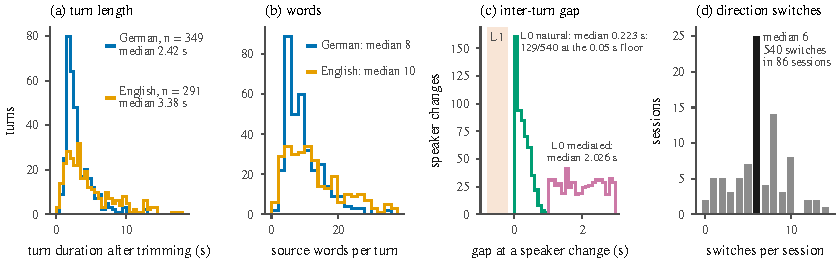
\includegraphics{figures/figA1_taxi_stats.pdf}
  \caption{\taxi statistics (86 sessions, 640 usable turns; aggregates only, as TAXI may not be redistributed). (a)~Turn duration after silence trimming (0.1\,s margins included), by source language. (b)~Source words per turn. (c)~Gaps drawn at the 540 speaker changes under L0 natural and L0 mediated; the shaded band of negative gaps marks where the planned L1 condition starts the next turn, 0.2--0.8\,s before the previous turn ends. (d)~Direction switches per session; the median (6) is drawn in black, and two sessions have no switch.}
  \label{fig:taxi-stats}
\end{figure}

\begin{figure}[htbp]
  \centering
  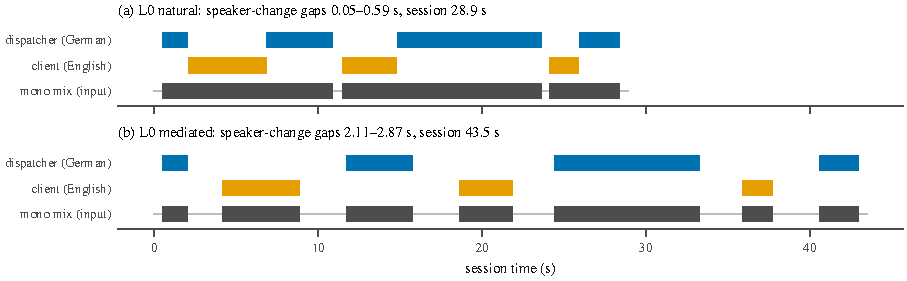
\includegraphics{figures/figA2_taxi_session.pdf}
  \caption{Session SES0104 (7 turns) rendered under (a)~L0 natural (speaker-change gaps 0.05--0.59\,s; session 28.9\,s, close to the median session of 29.023\,s) and (b)~L0 mediated (gaps 2.11--2.87\,s; session 43.5\,s). Lanes show the German dispatcher, the English client and the mono mix, which is all a system receives. Speech and turn order are real; the timing is synthetic. Only turn intervals are shown, no audio or text.}
  \label{fig:taxi-session}
\end{figure}

\paragraph{Caveats.}
Speech, content and turn order are real, but every gap is synthetic and the corpus has no overlap; overlap claims therefore rest on the L1 renders and on \syn (\cref{app:syn}). Turn intervals include the 0.1\,s margins, so the turn boundaries to which \eo and switch latency refer can be off by up to about 0.1\,s, and energy trimming may clip soft onsets; forced-aligned word times will check these boundaries.\draftnote{planned; the TAXI turns are not force-aligned yet}
Language and role are confounded (German is always the dispatcher), and the dispatcher opens 85 of the 86 sessions, a trivial prior for the first direction. The realistic wrappers therefore route by spoken-language identification (\cref{app:baselines}), and \syn renders both speaker--language assignments. Sessions SES0085 and SES0095 hold a single usable turn, in German; they have no direction switch and are excluded from switch metrics. Fourteen turns follow a turn of the same speaker, 9 because unusable turns in between were skipped and 5 because the two turns are adjacent in the source; a pause separates them, and they do not count as switches. Finally, TAXI serves only for evaluation: no threshold, operating point or model is tuned on it.

\paragraph{Release and reproducibility.}
TAXI is free of charge under a scientific licence, and a commercial licence is available; redistribution, even in part, requires the written permission of the copyright holders. We therefore release session and turn IDs, configurations, build scripts, checksums and per-turn scores keyed by turn ID, but no audio, text or system output derived from TAXI (\cref{tab:licences}). Each rendered session directory holds \texttt{mix.wav} (the single-channel system input), \texttt{2ch.wav} (one channel per speaker, for analysis and oracle diagnostics only) and \texttt{timeline.json} (turn intervals with margins, gaps, removed silence, transcripts and references). The channel order of \texttt{2ch.wav} follows the \texttt{channels} field of the timeline: channel~0 is the English client and channel~1 the German dispatcher.\draftnote{the package README states the reverse order; fix it before release}
Per-session seeds derived from the session IDs and Python's \texttt{random} module make the timelines identical on every platform (\cref{sec:bench}). \texttt{cstbench verify} requires the SHA-256 digest of every timeline (as sorted-key JSON) to match exactly and reports audio-hash differences separately, because audio hashes can depend on the numpy, scipy and libsndfile versions (the reference hashes were made with numpy 1.24.3, scipy 1.10.1 and libsndfile 1.2.2). A local rebuild matched 86/86 timeline digests and 86/86 \texttt{mix.wav} and \texttt{2ch.wav} hashes in both configurations. Released configurations are frozen, and any change gets a new name. With the corpus in \texttt{TAXI\_DIR} (one folder per session), the track is built and verified by
{\small
\begin{verbatim}
cstbench build-taxi --root TAXI_DIR --out OUT_DIR
cstbench verify --out OUT_DIR/taxi-natural  --reference checksums/taxi-natural.json
cstbench verify --out OUT_DIR/taxi-mediated --reference checksums/taxi-mediated.json
\end{verbatim}
}

\paragraph{Why TAXI.}
A real \task test set needs one conversation between at least two real speakers who use different languages, with shared multi-turn context, per-turn audio, the identity and language of each speaker, turn order and transcripts; reference translations, turn timing, session audio and per-speaker channels are desirable. Parallel speech read from scripts, separately recorded sides of a text dialogue, merged monolingual corpora and utterance sets whose order or context cannot be recovered do not qualify. \Cref{tab:corpora} checks the candidates against these requirements. MSLT \citep{federmann2016microsoft,federmann2017microsoft} was recorded from bilingual calls, but the English side of each call was discarded. DRAL \citep{ward2023dialogs,ward2024dialogs,avila2023towards} and mDRAL \citep{seamless2023seamless} pair fragments of one-language conversations with re-enactments in the other language. InCroMin \citep{cechovic2025corpus} records real meetings between people without a common language, but they talk through machine speech translation, each participant is recorded on a separate track, and no English--German pair is included. CS-Dialogue \citep{zhou2025csdialogue} holds about 104\,h of Mandarin--English code-switching without translations. The Verbmobil~II interpreter volumes, from the Verbmobil project \citep{wahlster2000verbmobil}, contain German--English and German--Japanese dialogues and a human-interpreter subset but require a paid licence, and the Fisher--CALLHOME Spanish--English corpus \citep{post2013improved} has a single source language. Among these candidates, only TAXI combines real two-language dialogues, human translations of both sides and free access for research. What it lacks, turn timing and overlap, is exactly what the renderer controls.

% =====================================================================
% Table A13 (tab:corpora): why TAXI. Real bilingual conversational speech
% resources checked against the requirements of a real CST test set.
% Included from App. A; the citation of every row is given in the text of App. A.
% Uses >{...}p{} columns (array package, loaded by makecell).
% =====================================================================
\begin{table}[htbp]
  \caption{Why \taxi: real bilingual conversational speech resources checked against the requirements of a real \task test set (citations in the text of \cref{app:taxi}). \cmark{} yes, \pmark{} partly, \xmark{} no; --: not assessed or not applicable.}
  \label{tab:corpora}
  \centering
  \footnotesize
  \setlength{\tabcolsep}{3pt}
  \begin{tabular}{@{}>{\raggedright\arraybackslash}p{2.2cm}>{\raggedright\arraybackslash}p{2.6cm}>{\raggedright\arraybackslash}p{1.4cm}>{\raggedright\arraybackslash}p{1.8cm}>{\raggedright\arraybackslash}p{2.0cm}>{\raggedright\arraybackslash}p{1.1cm}>{\raggedright\arraybackslash}p{2.0cm}>{\raggedright\arraybackslash}p{2.2cm}@{}}
    \toprule
    Corpus & Same conversation, two languages & Real spontaneous speech & Human translations & Per-turn audio\,/\,timing & Overlap & Access\,/\,licence & Verdict \\
    \midrule
    BAS TAXI 2.5
      & \cmark{} German dispatcher, English client
      & \cmark
      & \cmark{} both sides (TLN tier)
      & \pmark{} per-turn files; no timing (push-to-talk)
      & \xmark{} none
      & free scientific licence; no redistribution
      & \textbf{used} (real track) \\
    \addlinespace
    MSLT
      & \pmark{} bilingual calls; English side discarded
      & \cmark
      & \pmark{} released side only
      & one side only
      & --
      & --
      & unsuitable (one-sided release) \\
    \addlinespace
    DRAL\,/\,mDRAL
      & \xmark{} one language per conversation; fragments re-enacted in the other
      & \pmark{} originals only
      & \pmark{} spoken re-enactments
      & paired fragments
      & --
      & LDC (DRAL)
      & unsuitable (re-enacted) \\
    \addlinespace
    InCroMin
      & \cmark{} meetings mediated by machine speech translation
      & \cmark
      & \pmark{} corrected machine translations into English
      & per-participant tracks
      & --
      & CC BY 4.0
      & related work (12 languages, no English--German pair) \\
    \addlinespace
    CS-Dialogue
      & \pmark{} Mandarin--English code-switching within speakers
      & \cmark
      & \xmark
      & full dialogues
      & --
      & --
      & unsuitable (about 104\,h, no translations) \\
    \addlinespace
    Verbmobil~II interpreter volumes
      & \cmark{} German--English and German--Japanese; human-interpreter subset
      & \cmark
      & --
      & --
      & --
      & speech on paid media
      & not used \\
    \addlinespace
    Fisher--CALLHOME Spanish--English ST
      & \xmark{} one source language (Spanish)
      & \cmark
      & \cmark{} crowdsourced, into English
      & --
      & --
      & LDC
      & related (one source language) \\
    \bottomrule
  \end{tabular}
\end{table}


% =====================================================================
% Appendix B: CST-Bench-Syn construction and data card (one-column appendix).
% PLANNED: nothing of CST-Bench-Syn is built yet. The text specifies the design;
% tab:syn has blank cells for measured values and marks plan targets as targets.
% Never state plan estimates (hours, voice counts, cost) as facts.
% Holds the Syn detail that Sec. 4.1 leaves out: sources and their
% translation provenance, Korean consensus MT, TTS editions and QA,
% calibration split, translationese rule, release and licences, and the
% voice-consent rule (decision: "clone no real person's voice without
% consent"; Sec. 4 no longer repeats it, the Impact Statement does).
% =====================================================================
\section{CST-Bench-Syn Construction and Data Card}\label{app:syn}

\draftnote{planned: \syn is not built yet; this appendix specifies its construction, and every measured value in \cref{tab:syn} is pending}

\syn is an evaluation-only set of synthetic (TTS) speech. It adds what \taxi cannot provide: turn-end overlap that can be measured at the word level, a distant language pair, and both speaker--language assignments, which remove TAXI's first-speaker prior and its tie between language and role. It is not real conversation, does not meet the requirements for a real test set (\cref{app:taxi}) and is translationese on one side of every pair. We therefore draw only relative conclusions from it (gaps between protocols and system rankings, never absolute scores across directions or pairs) and test whether it ranks systems as \taxi does (\cref{tab:validity,fig:sim2real}). There is no training or development split: a calibration split of about 5\% of the sessions, disjoint from the evaluation sessions, is the only data on which wrapper thresholds and operating points are chosen, with one rule for all systems. \Cref{tab:syn} is the data card.

% =====================================================================
% Table A2 (tab:syn): CST-Bench-Syn data card. Included from App. B.
% PLANNED: the set is not built. Measured cells use \tbd (blank); the last
% column holds plan targets (not results). Known now: reference type, licences.
% Do not add hours, voice counts or costs: they are plan estimates, not facts.
% =====================================================================
\begin{table}[htbp]
  \caption{\syn data card (planned). The set is not built yet: blank cells will hold measured values, and the last column gives plan targets, which are not results. A session is one dialogue under one speaker--language assignment; every dialogue is rendered under both. The re-recognition error is the WER for English and German and the CER for Korean; turns above the target are re-synthesised. MT: machine translation; n/a: not applicable; --: no target.}
  \label{tab:syn}
  \centering
  \footnotesize
  \setlength{\tabcolsep}{4pt}
  \begin{tabular}{@{}lccccc@{}}
    \toprule
    & \multicolumn{2}{c}{\pair{En}{De}} & \multicolumn{2}{c}{\pair{Ko}{En}} & \\
    \cmidrule(lr){2-3}\cmidrule(lr){4-5}
    Statistic & XDailyDialog & BConTrasT & XDailyDialog & BConTrasT & Plan target \\
    \midrule
    \multicolumn{6}{@{}l}{\textit{Size}} \\
    Dialogues\,/\,sessions                    & \tbd & \tbd & \tbd & \tbd & -- \\
    Turns per direction                       & \tbd & \tbd & \tbd & \tbd & -- \\
    Speech per timing condition (h)           & \tbd & \tbd & \tbd & \tbd & -- \\
    Calibration split (\% of sessions)        & \tbd & \tbd & \tbd & \tbd & about 5 \\
    \midrule
    \multicolumn{6}{@{}l}{\textit{Speech}} \\
    Voices per language and edition           & \tbd & \tbd & \tbd & \tbd & -- \\
    Re-recognition error (\%)                 & \tbd & \tbd & \tbd & \tbd & $\leq 5$ \\
    Re-synthesised turns (\%)                 & \tbd & \tbd & \tbd & \tbd & -- \\
    Speaker cosine, same\,/\,other speaker    & \tbd & \tbd & \tbd & \tbd & -- \\
    TTS word times vs.\ forced alignment      & \tbd & \tbd & \tbd & \tbd & -- \\
    \midrule
    \multicolumn{6}{@{}l}{\textit{Text}} \\
    Reference type                            & human & human & \makecell{Ko: consensus MT\\En: human} & \makecell{Ko: consensus MT\\En: human} & -- \\
    Korean consensus pass rate (\%)           & n/a  & n/a  & \tbd & \tbd & $\geq 85$ \\
    Korean spot-check error rate (\%)         & n/a  & n/a  & \tbd & \tbd & -- \\
    Contamination-probe agreement             & \tbd & \tbd & \tbd & \tbd & -- \\
    Licence                                   & CC BY-NC-SA 4.0 & CC BY-SA 4.0 & CC BY-NC-SA 4.0 & CC BY-SA 4.0 & -- \\
    \bottomrule
  \end{tabular}
\end{table}


\paragraph{Pairs and speaker assignment.}
\pair{En}{De} is the main pair: it shares its languages with \taxi, which makes the sim-to-real comparison possible. \pair{Ko}{En} adds a distant word order. Every dialogue is rendered under both speaker--language assignments (speaker $A$ speaks the first language and $B$ the second, and vice versa), and the same dialogues serve both pairs, so differences between pairs come from the languages rather than from the content. We exclude German--Korean, which almost no baseline supports, and use English as the pivot.

\paragraph{Dialogues.}
XDailyDialog \citep{liu2023xdailydialog} provides professional translations of the everyday dialogues of DailyDialog \citep{li2017dailydialog}, and BConTrasT \citep{farajian2020findings} provides English--German versions of task-oriented Taskmaster-1 dialogues \citep{byrne2019taskmaster} between a customer and an agent in six domains, machine-translated into German and post-edited by native German speakers. Speaker $A$'s turns come from one language version of a dialogue and $B$'s from the other, so both share one context and the parallel version of each turn is its reference. We select dialogues of 6--16 turns and balance the domains, the turn lengths and the share of dialogues that contain numbers or named entities. XDailyDialog turns are short (about 11.5 tokens on average), so the selection favours multi-sentence turns, which leave room for turn-end overlap. No parallel corpus that cannot be redistributed is used.

\paragraph{Contamination.}
DailyDialog and Taskmaster-1 text may be in the pretraining data of the LLMs that serve as baselines and teachers. For each of them, a probe gives the opening turns of a selected dialogue, lets the model continue it and measures the agreement of the continuation with the original (\cref{tab:syn}). Generation prompts, models and seeds are released. No DailyDialog, Taskmaster-1 or TAXI text and no \syn dialogue or voice is used to train \model (\cref{sec:model}).

\paragraph{References.}
English--German references are the parallel versions of each turn: the English side is original, and the German side is a professional translation (XDailyDialog) or a post-edited machine translation (BConTrasT). Neither source contains Korean, so every Korean text, both the Korean turns that are synthesised and the Korean references of English turns, is translated from English by three independent systems: Qwen3.8-27B, MADLAD-400-10B-MT \citep{kudugunta2023madlad} and EXAONE-4.0 \citep{lgai2025exaone4}. A text passes if at least two of the three translations agree, as judged by MetricX-24 in its reference-free mode \citep{juraska2024metricx}, CometKiwi \citep{rei2022cometkiwi}, the LaBSE similarity \citep{feng2022labse} of back-translations, and matching numbers and named entities; text that fails is removed, and we report the pass rate. The released Korean text is the MADLAD-400 translation, as no evaluated system belongs to that model family: Qwen3.8-27B is also a baseline translator and the teacher of our commit targets (\cref{sec:model}), and EXAONE-4.0, whose licence restricts its outputs to non-commercial use, serves only in the agreement check, so its outputs are neither released nor used for training.\draftnote{fix the rule for text whose MADLAD-400 translation is the dissenting one}
Native Korean speakers annotate the errors in a fixed random sample with a light MQM-style scheme \citep{freitag2021experts}. \pair{Ko}{En} enters the main results only if at least 85\% of the Korean text passes and the speech meets the re-recognition target below; otherwise it is reported as a pilot. For \pair{En}{De}, silver references built in the same way test whether gold and silver references rank systems alike (\cref{tab:validity}). Gold and silver segments are aggregated separately, and reference-free CometKiwi is reported next to the reference-based metrics.

\paragraph{Speech synthesis and quality assurance.}
A commercial edition carries the main results: Azure neural TTS \citep{microsoft2026text} with native preset voices for en-US, de-DE and ko-KR, balanced by gender, and word boundaries from the synthesiser. An open edition, CosyVoice~3 \citep{du2025cosyvoice3} or Qwen3-TTS \citep{hu2026qwen3tts} (both with Apache-2.0 weights), covers a subset and tests whether the TTS engine changes system rankings (\cref{tab:validity}). A pilot of 50 sentences per language admits an engine only if its re-recognition error is at most 5\%. Each speaker keeps one voice throughout a dialogue. Voices are presets, designed voices or voices cloned from CC0 reference recordings; we clone no real person's voice without consent and no voice across languages. Every synthesised turn is re-recognised with Whisper-large-v3 \citep{radford2023robust} and Qwen3-ASR \citep{shi2026qwen3asr}; turns with a WER (CER for Korean) above 5\% are re-synthesised, and we report the error and the re-synthesis rate. Speaker consistency is measured by the cosine similarity of speaker embeddings within and between speakers. The synthesiser's word boundaries are compared with forced alignment (Qwen3-ForcedAligner; \citealp{shi2026qwen3asr}), and we report the distribution of their differences, because word-level overlap and the reference points of latency depend on these times.

\paragraph{Rendering and release.}
Sessions are rendered with the same renderer and rules as \taxi (\cref{sec:bench}) under L0 natural and L1, optionally also under L0 mediated, each with its own configuration name and checksums; overlap is measured on turn intervals and on word boundaries. Mixes are clean: noise and reverberation variants are outside this release, and a telephone-band variant is added only if \syn and \taxi rank systems differently. Each session comes with the mono mix, per-speaker channels (for analysis and oracle diagnostics only), a timeline with turn and word times, and references flagged as gold or silver. A data card discloses that the speech is synthetic and lists the sources, licences, generation models, prompts, seeds and QA results. CC BY-NC-SA 4.0 and CC BY-SA 4.0 are incompatible ShareAlike licences, so the XDailyDialog-based and the BConTrasT-based sessions form two subsets, each under the licence of its source (Taskmaster-1, on which BConTrasT builds, is CC BY 4.0). The commercial edition is synthesised only on a paid tier (\cref{tab:licences}). Instead of a fixed size in hours, \syn is sized by a power estimate from the variance of TAXI segment scores for the main comparisons, fixed before the test runs: a first tranche is built and extended only if its confidence intervals are too wide.

\paragraph{Out of scope.}
This release leaves out the parts of an earlier design that targeted interruptions and barge-in: episodes of two to four history turns, an interruption event and one or two resolution turns; information-causal event generation with three difficulty levels; sizing by at least 300 events per combination of event type, difficulty and pair, which implied about 10--12\,h per pair; partial references for interrupted turns; leakage checks for generated events; and a high-overlap condition with at least 25\% overlap. Interruptions remain future work (\cref{sec:conclusion}).

\paragraph{Limitations.}
TTS prosody lacks disfluencies, reactions to the partner and the Lombard effect; the dialogue text is largely planned rather than spontaneous; one side of every pair is translationese; the Korean references are silver; and wrapper thresholds calibrated on clean 16\,kHz TTS may suit telephone-band \taxi less well. Rank agreement with \taxi and between the two TTS editions (\cref{tab:validity}) indicates how far conclusions drawn on \syn transfer to real speech.

% =====================================================================
% Appendix C (app:scorer): scorer specification and metric validation
% (one-column appendix).
% Floats: Table A3 (tables/tab_sanity.tex), Table A7 (tables/tab_validity.tex),
% Fig. A4 (fig:sim2real, defined below).
% Implemented in the released scorer: submission format, normalisation,
% resegmentation, oracle turn-ID mode, BLEU, chrF, StreamLAAL, EndOffset,
% empty turns, wrong-language words given turn IDs. Everything else is
% planned and carries a \draftnote. Sanity-run numbers are preliminary (\prelim).
% Notation as in Secs. 3-4: b_n, e_n, L_n, r_n, h_n, tau_{n,j}, d_{n,j}, rho_n, J_n.
% Holds what Sec. 4 leaves out: normalisation, resegmentation algorithm,
% oracle mode (final results strip turn IDs), aggregation, penalised and
% matched-word variants, metric credits (SimulEval EndOffset/StartOffset,
% Seamless), the 540-of-554 switch caveat, the detector, transcript metrics,
% meta-evaluation and rank agreement (tau_b within direction x wrapper
% strata, averaged; n reported; threshold fixed before the test runs).
% Open user decisions, not applied: a time constraint on resegmentation,
% a "switch cost" metric, an "overrun rate" metric, COMET on raw Syn text,
% a minimum piece length for the language-ID rule, a TAXI-TTS control.
% =====================================================================
\section{Scorer Specification and Metric Validation}\label{app:scorer}

This appendix specifies \scorer precisely enough to reimplement it and describes how we test that its metrics measure what they are meant to measure. As in \cref{sec:task,sec:bench}, turn $n$ of a session of duration $T$ has speaker $s_n$, interval $[b_n,e_n]$, duration $L_n=e_n-b_n$ and a reference translation $r_n$ of $|r_n|$ words.
\draftnote{the released scorer implements the submission format, normalisation, resegmentation, oracle mode, BLEU, chrF, \laal, \eo, empty turns and wrong-language words given gold turn IDs; a pinned num2words, COMET, switch latency, the length ratio, the wrong-direction detector, the latency variants, the bootstrap and all transcript and speaker metrics are planned}

\subsection{Submission, clocks and normalisation}

\paragraph{Submission.}
A system submits one JSON line per committed piece with four fields: session ID, output language, emission time $t$ in seconds from the start of \texttt{mix.wav}, and text. The output language selects the direction (English output translates German speech), so no speaker or direction label is needed. Pieces are never retracted, and every line counts as committed. The scorer sorts the pieces of each session by emission time, keeping file order for ties, splits each normalised piece into words and gives every word the time of its piece. An optional gold turn ID per piece selects the oracle mode described below. Further fields are kept, and any of them can serve as the clock; pieces of unknown sessions are reported and ignored.

\paragraph{Clocks.}
On the ideal clock, $t$ is the audio consumed when the piece is committed; the computation-aware clock \citep{ma2020simulmt} adds processing time measured on fixed hardware (\cref{tab:ca-latency}). Unlike SimulEval \citep{ma2020simuleval}, which runs a policy on each source segment, \scorer sees only committed pieces and their times, so they can come from any streaming harness, such as simulstream \citep{gaido2025simulstream}, or from a unified model. On \taxi, turn intervals include the 0.1\,s margins of energy trimming (\cref{app:taxi}), which can move the reference points of every latency metric by up to about 0.1\,s.

\paragraph{Normalisation.}
Hypotheses and references are normalised alike, to the style of the TAXI references (lowercase, unpunctuated, numbers in words): (i)~Unicode NFC; (ii)~each number, i.e., a digit string with an optional decimal part, is spelled out with num2words in the output language, reading a decimal comma as a decimal point in German and dropping commas as thousands separators in the other languages; (iii)~lowercasing; (iv)~every character other than a letter, a digit, whitespace or a word-internal apostrophe becomes a space; (v)~splitting at whitespace. The scorer depends on a pinned num2words version, because without the package step~(ii) would be skipped silently.
\draftnote{planned: pinning num2words; the released scorer lists it only as an optional dependency (version 0.5 or later) and skips step (ii) silently if it is missing}

\paragraph{Quality.}
Per direction, BLEU \citep{papineni2002bleu} and chrF \citep{popovic2015chrf} are sacreBLEU corpus scores \citep{post2018call} over the turns of that direction, with default settings except for sacreBLEU's Korean tokenizer for BLEU into Korean; we report the signatures and two decimals. An empty turn enters as an empty hypothesis and lowers both scores. COMET with the wmt22-comet-da model \citep{rei2020comet,rei2022comet} scores the same resegmented turns, with the gold transcript as the source. A per-turn file holds each turn's source, hypothesis, reference and latencies; for \taxi, only per-turn scores keyed by turn ID are released (\cref{app:repro}).
\draftnote{planned: COMET inside the scorer and the Korean tokenizer; the released scorer leaves COMET to external tools reading the per-turn file}

\subsection{Resegmentation and oracle mode}

For each session and output language $\lambda$, \scorer assigns the hypothesis words to the turns $\mathcal{N}_\lambda$ that are translated into $\lambda$, with the minimum-edit-distance criterion of mwerSegmenter \citep{matusov2005evaluating} as used in stream-level evaluation \citep{iranzosanchez2021stream,papi2024streamatt}:
\begin{enumerate}
  \item order the hypothesis words $w_1,\dots,w_M$ by emission time;
  \item concatenate the normalised references $r_n$, $n\in\mathcal{N}_\lambda$, in dialogue order into $u_1,\dots,u_K$, and record the turn $o(k)$ of each reference word $u_k$;
  \item align $w_{1:M}$ to $u_{1:K}$ by word-level Levenshtein alignment with unit costs; on ties, the backtrace prefers a match or substitution to an insertion, and an insertion to a deletion;
  \item assign each $w_i$ aligned to some $u_k$, as a match or a substitution, to turn $o(k)$; assign each inserted word to the turn of the preceding aligned word or, if it precedes all aligned words, to the turn of the first aligned word.
\end{enumerate}
Turn $n$ thus receives the words $h_n$, with emission times $\tau_{n,1}\le\dots\le\tau_{n,|h_n|}$, and is empty if $h_n$ is empty. Resegmentation looks only at text, so a word can land in a turn that begins after the word was emitted, and latency on resegmented output inherits a segmentation-related bias \citep{polak2025better}.

\paragraph{Oracle mode.}
If every piece of a session and direction carries a gold turn ID, the scorer skips resegmentation and assigns words to their turns directly; words whose ID is not a turn of direction $\lambda$ count as wrong-language words and are not scored. This mode is only a diagnostic (\cref{sec:task}): scoring the same output both ways measures how much resegmentation alone moves the scores. Final results are resegmented, with any turn IDs removed from the hypotheses first; the preliminary rows of \cref{tab:main} were scored in oracle mode and will be re-scored.

\subsection{Latency}

For a non-empty turn $n$, let $d_{n,j}=\max(0,\tau_{n,j}-b_n)$ be the delay of its $j$-th word from the turn start, $\rho_n=L_n/\max(|h_n|,|r_n|)$ the rate, and $J_n$ the first $j$ with $d_{n,j}\ge L_n$, or $|h_n|$ if there is none. Then
\begin{align}
  \mathrm{StreamLAAL}_n &= \frac{1}{J_n}\sum_{j=1}^{J_n}\bigl(d_{n,j}-(j-1)\,\rho_n\bigr), \label{eq:app-laal}\\
  \mathrm{EndOffset}_n &= \tau_{n,|h_n|}-e_n, \label{eq:app-eo}\\
  \mathrm{SwitchLatency}_n &= d_{n,1}\qquad\text{for } n>1 \text{ with } s_n\neq s_{n-1}. \label{eq:app-switch}
\end{align}
\Cref{eq:app-laal} is LAAL \citep{papi2022overgeneration}, the length-adaptive form of Average Lagging \citep{ma2019stacl}, applied to resegmented turns, i.e., \laal \citep{papi2024streamatt}. Two cases show what the metrics separate. If a turn's translation is committed at $e_n$, every delay equals $L_n$, so $J_n=1$, $\mathrm{StreamLAAL}_n=L_n$ and $\mathrm{EndOffset}_n=0$: offline systems on oracle turns score the mean turn duration, 4.624\,s for \ende and 3.086\,s for \deen on \taxi. If instead the $j$-th of the $|r_n|$ reference words is committed at $b_n+jL_n/|r_n|$, then $\mathrm{StreamLAAL}_n=L_n/|r_n|$, the duration of one word, while $\mathrm{EndOffset}_n$ is still 0. \laal thus measures the lag within a turn and \eo the wait after it. \eo is negative if a turn's output ends before the speaker does, through anticipation or truncation, so we always report it with quality and length ratio. Neither waiting metric is new: \eo is SimulEval's EndOffset, the delay of the last output after the end of the source \citep{ma2020simuleval}, which SeamlessStreaming also reports as its ending offset \citep{seamless2023seamless}, computed here per turn; switch latency (\cref{eq:app-switch}) is SimulEval's StartOffset, the delay of the first output, taken only at turns that change direction. It is undefined for the first turn of a session, so the two single-turn \taxi sessions contribute none; and as 540 of the 554 later \taxi turns follow a speaker change, switch latency on \taxi is close to the first-word delay of all later turns.

\paragraph{Aggregation.}
Per direction, we report the mean, median and 90th percentile over non-empty turns, to three decimals. The median averages the two middle values of an even count, and the 90th percentile of $m$ values is the sorted value at the 0-based index $\min(m-1,\lfloor 0.9m\rfloor)$. The empty-turn rate is reported next to every latency.

\paragraph{Penalised variant.}
Averaging over non-empty turns lets a system improve its latency by dropping hard turns. The penalised variant therefore scores an empty turn as if its whole reference were committed at the session end: $\mathrm{EndOffset}_n=T-e_n$ and $\mathrm{StreamLAAL}_n=\mathrm{SwitchLatency}_n=T-b_n$. On the ideal clock no piece comes later than $T$, so these are the worst values any output can obtain, and dropping a turn never lowers its latency.

\paragraph{Exactly matched words.}
Unrelated output can lower \laal (row~2 of \cref{tab:sanity}); one mechanism is that a word assigned to a turn that begins after the word was emitted gets delay 0. We therefore also report \cref{eq:app-laal,eq:app-eo} with $h_n$ restricted to the words that exactly match their aligned reference word, so that unrelated words cannot contribute.
\draftnote{planned: switch latency, the penalised variant and the matched-word variant}

\subsection{Errors and auxiliary outputs}

\paragraph{Empty turns and length ratio.}
A turn is empty if no word is assigned to it. Per direction, we report the share of empty turns and the ratio of hypothesis to reference words.
\draftnote{planned: the length ratio; the released scorer reports only the numbers of turns and of empty turns}

\paragraph{Wrong-direction words.}
In oracle mode, wrong-direction words are the wrong-language words defined above. Without turn IDs, a piece $(t_i,\lambda_i,y_i)$ is checked against the turns open at its emission time, $\mathcal{A}(t_i)=\{n: b_n\le t_i\le e_n+W\}$, with a window $W$ fixed before any system is scored. All words of the piece are wrong-direction words if
(a)~\emph{wrong channel}: $\mathcal{A}(t_i)$ is non-empty and all its turns are spoken in $\lambda_i$, so no open turn needs a translation into $\lambda_i$;
(b)~\emph{wrong language}: a text language identifier restricted to the session's two languages assigns $y_i$ to the language other than $\lambda_i$; or
(c)~\emph{copy-through}: $y_i$ is closer to the transcript of an open turn spoken in $\lambda_i$ than to the reference of every open turn translated into $\lambda_i$, where the distance from $y_i$ to a text is the smallest word edit distance between $y_i$ and a span of that text, divided by the length of $y_i$.
Under turn-end overlap, turns in both languages are open at once, so (a) cannot fire and (b) and (c) decide. Rows~2 and~8 of \cref{tab:sanity} test (b) and (c), and the delayed rows check that late but correct output is not flagged. We report wrong-direction words as a percentage of all committed words and compare the detector with the oracle-mode count wherever turn IDs exist.
\draftnote{planned: the detector, its window $W$ and the text language identifier; the released scorer counts wrong-language words only given gold turn IDs}

\paragraph{Transcripts and speakers.}
For systems with a transcript channel, we report WER per language after the same normalisation; cpWER \citep{watanabe2020chime}, which compares each speaker's concatenated words under the best mapping between hypothesis and reference speakers, so that arrival-order labels need no fixed identity; and its time-constrained variant tcpWER from MeetEval \citep{vonneumann2023meeteval}. For Korean, cpCER applies cpWER to characters instead of words. DER uses collars of 0 and 0.25\,s at 80\,ms resolution. The main text reports WER, cpWER (cpCER on \syn \pair{Ko}{En}) and DER (\cref{tab:aux}); tcpWER and DER without a collar are in \cref{app:results}.
\draftnote{planned}

\paragraph{Speaker-attributed BLEU.}
DiariST scores translations per speaker after mapping hypothesis speakers to reference speakers \citep{yang2024diarist}. In \task each speaker uses one language, so the reference translations of speaker~$A$ are exactly those of direction $\ell_A\to\ell_B$. For a system that labels its translations with speakers, speaker-attributed BLEU therefore scores the same hypothesis--reference pairs as per-direction BLEU whenever every piece labelled~$A$ is in $\ell_B$ and every piece labelled~$B$ is in $\ell_A$. The two differ only on pieces whose label contradicts their language; these are attribution or direction errors, which the wrong-direction rate and cpWER already count. We therefore compute speaker-attributed BLEU only as a consistency check for systems with speaker labels.

\subsection{Metric meta-evaluation}

% =====================================================================
% Table A3 (tab:sanity): metric meta-evaluation by controlled perturbations
% of the reference output on CST-Bench-TAXI, L0 natural. Included from App. C,
% which describes how every row is constructed.
% Rows 1-2: preliminary scorer sanity runs (\prelim; to be re-run and recorded).
% All other cells are pending (\tbd). W counts words (not a percentage).
% Rows 3-5 state their delay (+0.5/+1/+2 s); the symbol Delta is avoided because
% it is the chunk length in Sec. 5 and a COMET difference in Tables 4 and 6.
% =====================================================================
\begin{table}[t]
  \caption{Metric meta-evaluation on \taxi, L0 natural: controlled perturbations of the reference translations, with the change expected for each metric fixed in advance (construction of each row in \cref{app:scorer}). Q: BLEU and chrF; L: mean \laal (s); E: mean \eo (s), both over non-empty turns; W: number of wrong-direction words; $L_n$, $|r_n|$: duration and reference length of turn $n$; $=$: unchanged; $\uparrow$\,/\,$\downarrow$: increases\,/\,decreases. $^\dagger$Preliminary; to be re-run under the final protocol. $^\ast$The current scorer counts such words only given gold turn IDs. Blank cells are pending.}
  \label{tab:sanity}
  \centering
  \footnotesize
  \setlength{\tabcolsep}{3pt}
  \begin{tabular}{@{}rllccccccc@{}}
    \toprule
    & & & \multicolumn{3}{c}{\ende} & \multicolumn{3}{c}{\deen} & \\
    \cmidrule(lr){4-6}\cmidrule(lr){7-9}
    & Perturbation & Expected change & BLEU\,/\,chrF & L & E & BLEU\,/\,chrF & L & E & W \\
    \midrule
    1  & Reference at turn end
       & \makecell[l]{Q $=100$; L $=$ mean $L_n$;\\E $=0$; W $=0$}
       & \prelim{100.0\,/\,100.0} & \prelim{4.624} & \prelim{0.0}
       & \prelim{100.0\,/\,100.0} & \prelim{3.086} & \prelim{0.0} & \prelim{0} \\
    2  & \makecell[l]{Source transcript passed\\through untranslated}
       & \makecell[l]{Q $\approx0$; L, E not below\\row 1; W $=$ all words}
       & \prelim{2.38\,/\,27.34} & \prelim{4.366} & \prelim{2.576}
       & \prelim{0.39\,/\,21.86} & \prelim{2.276} & \prelim{1.421} & \prelim{0}$^\ast$ \\
    3  & Row 1 delayed by 0.5\,s & Q $=$; L, E $+0.5$\,s; W $=0$ & \tbd & \tbd & \tbd & \tbd & \tbd & \tbd & \tbd \\
    4  & Row 1 delayed by 1\,s   & Q $=$; L, E $+1$\,s; W $=0$ & \tbd & \tbd & \tbd & \tbd & \tbd & \tbd & \tbd \\
    5  & Row 1 delayed by 2\,s   & Q $=$; L, E $+2$\,s; W $=0$ & \tbd & \tbd & \tbd & \tbd & \tbd & \tbd & \tbd \\
    6  & \makecell[l]{Reference spread evenly\\over the turn}
       & \makecell[l]{Q $=$; L $=$ mean $L_n/|r_n|$;\\E $=0$; W $=0$}
       & \tbd & \tbd & \tbd & \tbd & \tbd & \tbd & \tbd \\
    7  & \makecell[l]{Row 6 without the last\\third of each turn}
       & \makecell[l]{vs.\ row 6: Q $\downarrow$; L $=$;\\E $\downarrow$ (below 0); W $=0$}
       & \tbd & \tbd & \tbd & \tbd & \tbd & \tbd & \tbd \\
    8  & \makecell[l]{Turns merged across a\\speaker change (VAD)}
       & \makecell[l]{Q $\downarrow$; E $\uparrow$; W $\uparrow$;\\more empty turns}
       & \tbd & \tbd & \tbd & \tbd & \tbd & \tbd & \tbd \\
    9  & \makecell[l]{Output of 10\% of turns\\dropped}
       & \makecell[l]{Q $\downarrow$; L, E $\approx$ row 1;\\10\% empty turns}
       & \tbd & \tbd & \tbd & \tbd & \tbd & \tbd & \tbd \\
    10 & \makecell[l]{Rows 1, 3--7, 9 with gold\\turn IDs: largest change}
       & 0 for every metric
       & \tbd & \tbd & \tbd & \tbd & \tbd & \tbd & \tbd \\
    \bottomrule
  \end{tabular}
\end{table}


We perturb the reference output on \taxi L0 natural and check that BLEU, chrF, \laal, \eo and the wrong-direction count each move as expected while the others stay put (\cref{tab:sanity}); the expected changes are fixed in advance. COMET and switch latency are not yet in the table, as the released scorer does not compute them. Row~1 commits every reference translation at its turn end. Row~2 emits each turn's source transcript as its translation, as a system that passes speech through untranslated would. Rows~3--5 delay row~1 by 0.5, 1 and 2\,s. Row~6 commits the $j$-th reference word of turn $n$ at $b_n+jL_n/|r_n|$, and row~7 drops the last $\lfloor|r_n|/3\rfloor$ words of every turn of row~6. Row~8 simulates a VAD that merges two turns across a speaker change, at a seeded subset of speaker changes: the first turn's reference is committed at the end of the second turn, followed on the same channel by the second turn's source transcript, as if the merged segment had been routed by the first turn's language. Row~9 removes the output of a seeded 10\% of turns. Row~10 rescores rows~1, 3--7 and~9, whose words all come from the right turns, with gold turn IDs and reports the largest change. No final system result is reported until every row behaves as expected or the deviation is explained; the preliminary system results have not yet passed this check and will be re-run. We repeat the comparison of row~10 for every system run under the oracle wrapper, whose pieces carry turn IDs.

Rows~1 and~2 exist so far only as preliminary runs ($^\dagger$; to be re-run under the final protocol). Row~1 behaves as derived above: BLEU and chrF are \prelim{100.0}, \eo is \prelim{0.0}\,s, no word counts as wrong, and the mean \laal equals the mean turn duration (\prelim{4.624}\,s for \ende, \prelim{3.086}\,s for \deen). Row~2 drives BLEU down to \prelim{2.38} for \ende and \prelim{0.39} for \deen, while chrF keeps \prelim{27.34} and \prelim{21.86} from shared character n-grams. However, it \emph{lowers} the mean \laal below that of the reference (\prelim{4.366} vs.\ \prelim{4.624}\,s for \ende; \prelim{2.276} vs.\ \prelim{3.086}\,s for \deen) and raises the mean \eo to \prelim{2.576} and \prelim{1.421}\,s, presumably because resegmentation spreads the untranslated words over neighbouring turns; and without turn IDs, the current scorer counts none of these words as wrong. These two failures motivate the matched-word latency, the rule to show latency only next to quality, length ratio and empty turns, and the wrong-direction detector. In addition, five unit tests check normalisation, resegmentation, LAAL, oracle versus resegmented scoring and the command-line interface on toy sessions; for instance, an oracle hypothesis scores BLEU 100.0 with a mean \eo of 0.0\,s, and a two-word turn reaches chrF 100.0.
\draftnote{re-run rows 1--2 under the final protocol and record how the row-2 hypothesis is time-stamped}

\subsection{Rank agreement and sim-to-real validity}

% =====================================================================
% Table A7 (tab:validity): rank-agreement checks behind the validity claims
% (sim-to-real, TTS edition, silver references, render seeds, metric choice).
% Included from App. C. Nothing has been run yet: every cell is \tbd.
% tau_b is computed within direction x wrapper strata and averaged, so that
% wrapper and direction differences cannot inflate agreement (review); the
% "oracle--realistic gap" row ranks systems by their gap on each set, as the
% paper's claims rest on gaps. A TAXI-TTS control row would be a new
% experiment (user decision) and is not listed.
% =====================================================================
\begin{table}[t]
  \caption{Validity of system rankings (TAXI: \taxi; Syn: \syn; all L0 natural). Each row ranks the same systems at their main operating points in two ways; Kendall's $\tau_b$ is computed within each direction $\times$ wrapper stratum (each direction for gaps) and averaged over strata, with a 95\% CI from 2,000 session-bootstrap resamples; $n$ counts the ranked configurations. For render seeds, $\tau_b$ is the smallest pairwise value among the three renders; \cref{app:scorer} also compares their standard deviation with the CI width. Blank cells are pending.}
  \label{tab:validity}
  \centering
  \small
  \setlength{\tabcolsep}{5pt}
  \begin{tabular}{@{}llccc@{}}
    \toprule
    Comparison & Configurations compared & $n$ & Kendall's $\tau_b$ & 95\% CI \\
    \midrule
    \multicolumn{5}{@{}l}{\textit{Speech, construction and rendering (chrF rankings)}} \\
    TAXI vs.\ Syn \pair{En}{De}                 & those run on both sets  & \tbd & \tbd & \tbd \\
    \quad oracle--realistic gap                 & same, ranked by gap     & \tbd & \tbd & \tbd \\
    Commercial vs.\ open TTS edition           & Syn subset              & \tbd & \tbd & \tbd \\
    Gold vs.\ silver references                & Syn \pair{En}{De}       & \tbd & \tbd & \tbd \\
    Render seeds 1--3 (chrF and \eo)           & TAXI                    & \tbd & \tbd & \tbd \\
    \midrule
    \multicolumn{5}{@{}l}{\textit{Metric choice}} \\
    \laal vs.\ \eo                             & TAXI                    & \tbd & \tbd & \tbd \\
    \laal vs.\ LongYAAL                        & TAXI                    & \tbd & \tbd & \tbd \\
    COMET vs.\ chrF                            & TAXI                    & \tbd & \tbd & \tbd \\
    \bottomrule
  \end{tabular}
\end{table}


Several choices could change our conclusions without changing any system: synthetic instead of real speech, the TTS engine, silver instead of human references, the random render, and the metric. \Cref{tab:validity} measures each by Kendall's $\tau_b$ between two rankings of the same systems at their main operating points. Pooling wrappers and directions would inflate agreement, as their large differences recur in both rankings, so we compute $\tau_b$ within each combination of direction and wrapper and average it over these strata; we report the number $n$ of ranked configurations and a 95\% CI from 2,000 bootstrap resamples of sessions, drawn independently in each set when two sets are compared (\cref{app:repro}).

\paragraph{Synthetic versus real speech.}
The main check ranks all systems that run on both sets by chrF on \taxi and on \syn \pair{En}{De}, both under L0 natural, so that only the speech and the dialogues differ (\cref{fig:sim2real}); as our claims rest on oracle--realistic gaps, it also ranks the systems by their gap on each set, within each direction. We fix a threshold $\tau^\ast$ (\tbdtext) before the test runs: if the lower CI bound reaches $\tau^\ast$, \syn may rank systems on its own; otherwise we report the disagreement as a finding, use \syn only for contrasts within one set, such as oracle versus realistic wrappers or L0 versus L1, and test whether a telephone-band rendering of \syn restores agreement. The commercial and the open TTS edition are compared in the same way on a subset of \syn.

\begin{figure}[t]
  \centering
  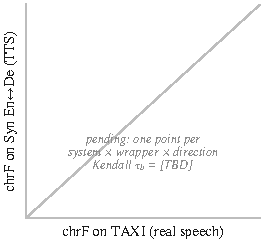
\includegraphics{figures/figA4_sim2real.pdf}
  \caption{Sim-to-real agreement: chrF of each system, wrapper and direction at its main operating point on \taxi (real speech) and on \syn \pair{En}{De} (TTS), both under L0 natural. Hollow markers: realistic wrapper; grey line: identity. Kendall's $\tau_b$, averaged over direction and wrapper strata, is annotated in the panel; its bootstrap CI is in \cref{tab:validity}.
  \protect\draftnote{placeholder; the points appear once the baselines have run on both sets}}
  \label{fig:sim2real}
\end{figure}

\paragraph{References and renders.}
To test how far silver references can rank systems, we rescore \syn \pair{En}{De} against silver references produced like the Korean ones (\cref{app:syn}) instead of the human references. To test render noise, we re-render \taxi L0 natural with seeds 1--3 under new configuration names and compare the standard deviation of chrF and \eo across seeds with the bootstrap CI width; \cref{tab:validity} lists the smallest pairwise $\tau_b$ among the three renders.

\paragraph{Metrics.}
\laal and \eo measure different waits, so a low $\tau_b$ between them is a finding rather than a validity failure: it shows that the listener's wait reorders systems. We keep \laal as the main latency metric because it was the latency metric of the IWSLT~2025 simultaneous track \citep{abdulmumin2025findings} and shares the resegmentation of our quality metrics. LongYAAL \citep{polak2025better}, computed on SoftSegmenter resegmentation in OmniSTEval and designed against the segmentation-related bias of resegmented latency, was the primary latency metric of IWSLT~2026, which reported \laal for comparison \citep{adelani2026speech}; we report how well the two agree. Rankings by string metrics alone can mislead \citep{kocmi2021ship}, which favours COMET, but the TAXI references are lowercase and unpunctuated. COMET is therefore primary on \taxi only if the lower CI bound of $\tau_b$ between its ranking and that of chrF reaches $\tau^\ast$; otherwise chrF is.
\draftnote{planned: every row of \cref{tab:validity} and the points of \cref{fig:sim2real}}

% =====================================================================
% Appendix D (app:baselines): baselines, wrappers, operating points, prompts
% (one-column appendix). Float: Table A4 (tables/tab_baselines.tex).
% Implemented: the offline systems with oracle input (offline baseline script
% of the cst-bench package; prompt, max_new_tokens 160 and batch 16 quoted
% from it). Planned: the streaming variant with oracle input, both wrappers,
% the streaming baselines, the decoupled twin and the operating points (each
% marked with \draftnote). Systems with oracle input are not called bounds.
% =====================================================================
\section{Baselines and Wrappers}\label{app:baselines}

\Cref{tab:baselines} lists the translation systems of \cref{sec:exp}. All of them are scored by \scorer from committed, time-stamped pieces (\cref{app:scorer}); this appendix describes how each system turns a session into pieces, how its latency settings are chosen, and which prompts the LLM-based systems use. We use public checkpoints without fine-tuning on \task data; the only tuning data is the \syn calibration split, and nothing is tuned on \taxi. Seed LiveInterpret~2.0 \citep{cheng2025seed}, a closed system, covers only Chinese--English, which \bench lacks, so we discuss it but do not run it.
\draftnote{implemented: the offline systems with oracle input, whose \taxi scores are preliminary; planned: the streaming variant with oracle input, both wrappers, the streaming baselines, the decoupled twin and the operating points}

% =====================================================================
% Table A4 (tab:baselines): baseline configurations. Included from App. D.
% Known cells only: checkpoints and parameter counts given by the model names
% or the model cards, offline settings, directions, wrappers, and the
% licences already verified (Qwen3.8-27B, Qwen3-ASR, Nemotron 3.5 ASR,
% Hibiki-Zero). Everything else, including both values of every latency
% knob, is \tbd. System names follow Table 3 (tab:main) and Table 6
% (tab:ablation). Systems with oracle input are not called bounds.
% 600M (model card) and 638M (measured) count the whole Nemotron 3.5 ASR
% model, RNN-T decoder included, not its encoder alone.
% =====================================================================
\begin{table}[tp]
  \caption{Baseline configurations, named as in \cref{tab:main,tab:ablation} (LLM: Qwen3.8-27B). Params: recognition plus translation models (B: billions; \model: total; its encoder comes from Nemotron~3.5 ASR Streaming 0.6B, which has 600M parameters per its model card and 638M as measured, RNN-T decoder included). Directions: \pair{En}{De} on \taxi and, for systems with a Korean entry, on \syn; \pair{Ko}{En} on \syn only. Policy: when text is committed; LA-2: LocalAgreement-2. Latency knob: the setting swept on the \syn calibration split; its two values (low and high latency) are chosen by the rule of \cref{app:baselines} and are pending. Wrappers: O oracle segmentation, R realistic (VAD and language-ID routing), --~none (the system handles the whole mix). Not listed: the diarization cascades of \cref{tab:aux}, which do not translate (\cref{app:baselines}). $^\ast$Optional; InfiniSST only if its weights are public; Hibiki-Zero is scored on its text output. Blank cells are pending.}
  \label{tab:baselines}
  \centering
  \fontsize{8}{9.5}\selectfont % 8pt (ICML \footnotesize is 9pt): fits the width
  \setlength{\tabcolsep}{2.5pt}
  \begin{tabular}{@{}llllllll@{}}
    \toprule
    System & Checkpoint\,/\,version & Params & Directions & Policy & \makecell[l]{Latency knob\\(two points)} & Wrappers & Licence \\
    \midrule
    \multicolumn{8}{@{}l}{\textit{Offline, oracle input: gold turns, each translated after it ends}} \\
    Gold$\to$LLM
      & Qwen3.8-27B & 27B
      & \makecell[l]{\pair{En}{De}\\\pair{Ko}{En}} & turn end & -- & O & Apache-2.0 \\
    ASR$\to$LLM
      & \makecell[l]{Qwen/Qwen3-ASR-1.7B;\\Qwen3.8-27B} & 1.7B\,+\,27B
      & \makecell[l]{\pair{En}{De}\\\pair{Ko}{En}} & turn end & -- & O & Apache-2.0 \\
    Whisper ST
      & openai/whisper-large-v3 & \tbd
      & \makecell[l]{\dir{De}{En}\\\dir{Ko}{En}} & turn end & -- & O & \tbd \\
    \midrule
    \multicolumn{8}{@{}l}{\textit{Streaming, oracle input: gold transcripts with forced-aligned word times; non-causal unit choice}} \\
    Gold$\to$LLM (MU2)
      & Qwen3.8-27B & 27B
      & \pair{En}{De} & MU2 units & \makecell[l]{one point\\(chrF $\geq$ 50)} & O & Apache-2.0 \\
    \midrule
    \multicolumn{8}{@{}l}{\textit{Pipelines built from single-direction systems}} \\
    \makecell[l]{Consecutive\\cascade}
      & \makecell[l]{Silero VAD; LID;\\Qwen3-ASR-1.7B;\\Qwen3.8-27B} & 1.7B\,+\,27B
      & \makecell[l]{\pair{En}{De}\\\pair{Ko}{En}} & VAD endpoint & \makecell[l]{endpoint\\silence} & R & \tbd \\
    SeamlessStreaming
      & \tbd & \tbd
      & \makecell[l]{\pair{En}{De}\\\pair{Ko}{En}} & EMMA & \makecell[l]{decision\\threshold} & O, R & \tbd \\
    2$\times$SeamlessStreaming
      & as above & \tbd
      & \pair{En}{De} & EMMA & as above & -- & \tbd \\
    \makecell[l]{Streaming\\cascade}
      & \makecell[l]{nvidia/nemotron-3.5-\\asr-streaming-0.6b;\\Qwen3.8-27B} & 0.6B\,+\,27B
      & \makecell[l]{\pair{En}{De}\\\pair{Ko}{En}} & LA-2 & \makecell[l]{ASR chunk,\\update step} & O, R & \makecell[l]{OpenMDW-1.1;\\Apache-2.0} \\
    M4T v2 + AlignAtt
      & SeamlessM4T v2 & \tbd
      & \pair{En}{De} & AlignAtt & frames $f$ & O, R & \tbd \\
    \makecell[l]{Canary-1B-v2\\+ AlignAtt$^\ast$}
      & Canary-1B-v2 & 1B
      & \pair{En}{De} & AlignAtt & frames $f$ & O, R & \tbd \\
    StreamSpeech
      & \tbd & \tbd
      & \dir{De}{En} & learned & chunk size & O, R & \tbd \\
    Hibiki-Zero$^\ast$
      & \makecell[l]{hibiki-zero-3b-\\pytorch-bf16} & 3B
      & \dir{De}{En} & learned & \tbd & O, R & \makecell[l]{CC BY-NC-SA\\4.0} \\
    InfiniSST$^\ast$
      & \tbd & \tbd
      & \dir{En}{De} & learned (LLM) & \tbd & O, R & \tbd \\
    \midrule
    \multicolumn{8}{@{}l}{\textit{Controls in the ablations (\cref{tab:ablation})}} \\
    Decoupled twin
      & \makecell[l]{\model M1; separate\\1.7B-thinker pass} & \tbd
      & \pair{En}{De} & \makecell[l]{MU2 units,\\delay $\delta_t$} & $\delta_t$ & -- & \makecell[l]{OpenMDW-1.1;\\Apache-2.0} \\
    \makecell[l]{Same-backbone cascade\\(M1$\to$LLM)}
      & \makecell[l]{\model M1;\\Qwen3.8-27B} & 2,336M\,+\,27B
      & \pair{En}{De} & LA-2 & update step & -- & \makecell[l]{OpenMDW-1.1;\\Apache-2.0} \\
    \makecell[l]{Size-matched cascade\\(ASR$\to$1.7B LLM)}
      & \makecell[l]{Qwen3-ASR-1.7B;\\LLM of $\approx$1.7B} & 1.7B\,+\,$\approx$1.7B
      & \pair{En}{De} & LA-2 & update step & R & \tbd \\
    \midrule
    \multicolumn{8}{@{}l}{\textit{Ours}} \\
    \model
      & \makecell[l]{Nemotron 3.5 encoder;\\Qwen3-ASR-1.7B\\thinker} & 2,336M
      & \makecell[l]{\pair{En}{De}\\\pair{Ko}{En}} & \makecell[l]{MU2 units,\\delay $\delta_t$} & $\delta_t$ & -- & \makecell[l]{OpenMDW-1.1;\\Apache-2.0} \\
    \bottomrule
  \end{tabular}
\end{table}


\paragraph{Offline systems with oracle input.}
Each gold turn is cut from \texttt{mix.wav} at its reference interval, 0.1\,s margins included, and translated after it ends, one turn per prompt and without dialogue history. Qwen3-ASR-1.7B \citep{shi2026qwen3asr} transcribes the turn with its language given, and Qwen3.8-27B translates this transcript, or the gold transcript, from the user message
\begin{quote}\small\ttfamily\raggedright
Translate this \{src\_lang\} utterance from a phone conversation into \{tgt\_lang\}. Output only the \{tgt\_lang\} translation.
\end{quote}
followed by a blank line and the turn's text; the placeholders are English names of the languages, such as \texttt{German}. Decoding is greedy with at most 160 new tokens and the model's reasoning mode switched off, and the first line of the answer is kept. Whisper-large-v3 \citep{radford2023robust} translates German turns, and on \syn Korean turns, into English with its translation task and the source language given; it cannot translate into German. All models process batches of 16 turns. Every piece carries its turn ID and is stamped at the turn end $e_n$, so on the ideal clock \eo is 0 and \laal equals $L_n$ (\cref{app:scorer}). The preliminary \taxi scores of these systems were computed in the scorer's oracle mode, by turn ID and without resegmentation, and will be re-scored with resegmentation under the final protocol. We do not call these systems bounds: they translate without dialogue history, and on \deen Whisper ST already scores above Gold$\to$LLM in BLEU (\cref{tab:main}). The computation-aware clock adds the per-turn compute, measured as the time of a batch divided by its size and therefore approximate; \cref{tab:ca-latency} re-measures it without batching. The WER of the ASR transcripts is computed after the scorer's normalisation.

\paragraph{Streaming variant with oracle input.}
To show what the commit policy costs and saves when recognition and segmentation are perfect, Gold$\to$LLM (MU2) reveals gold transcripts with forced-aligned word times (Qwen3-ForcedAligner; \citealp{shi2026qwen3asr}) word by word to Qwen3.8-27B, which commits translations at verified meaning units (MU2; \cref{sec:model}), accepting a unit if its chrF against the aligned part of the full translation is at least 50. A unit is stamped when its last source word ends, and the rest of a turn is flushed at the turn end. As units are chosen with the whole turn in view, this system is non-causal; it runs only under the oracle wrapper and so never becomes the reference pipeline $P$ of \cref{sec:exp-setup}.
\draftnote{planned; the German minimum unit is set on held-out data before the run}

\paragraph{Oracle wrapper.}
A single-direction system runs as two instances, one per target language. The wrapper cuts each gold turn $[b_n,e_n]$ from the mono mix, so that under L1 the cut also contains the overlapping speech of the other speaker, and streams it in real time to the instance that translates into the other speaker's language. Instances are reset at every turn and receive no dialogue history. A piece emitted after the instance has consumed $u$ seconds of the turn is stamped $b_n+u$ on the ideal clock, plus compute time on the computation-aware clock, and carries the turn ID. The main scores are computed with the turn IDs removed, so that the scorer resegments oracle-wrapper output like any other; scoring with them (oracle mode, \cref{app:scorer}) is a diagnostic of how much resegmentation alone moves the scores. Cutting the turn from its speaker's channel of \texttt{2ch.wav} instead, in the channel order recorded in the timeline, gives the oracle-separation variant of \cref{tab:factorial}.
\draftnote{planned}

\paragraph{Realistic wrapper.}
The realistic wrapper receives only the mix and the language pair. Silero VAD \citep{silero2024silero} segments the stream online: a segment opens at a detected speech onset and closes after a minimum silence. A spoken-language identifier restricted to the session's two languages labels each segment from its onset and updates the label as audio arrives. The segment is streamed to the instance that translates into the other language and is re-routed to the other instance if the label flips; text already committed stays. Pieces are stamped from the segment onset as in the oracle wrapper. As identifier we use the automatic language detection of Nemotron~3.5 ASR \citep{nvidia2026nemotron35asr}, or the language identification of Qwen3-ASR \citep{shi2026qwen3asr} if the former proves less accurate on the calibration split. The VAD's speech-probability threshold, minimum silence and speech padding and the identifier's settings are fixed once on that split, for all systems. As the split is clean 16\,kHz TTS, these settings may suit telephone-band \taxi less well (\cref{app:syn}). A short minimum silence splits turns at pauses, whereas a long one merges turns across the short L0 natural gaps (median drawn gap 0.223\,s on \taxi, to which the 0.1\,s turn margins add up to 0.2\,s of silence; \cref{sec:bench-timing}); under L1, the VAD hears one continuous segment across the speaker change, so the second turn inherits the first turn's route unless the label flips. Sweeps of the minimum silence on \taxi show how sensitive the realistic wrapper is to this setting; they serve analysis only, not tuning. The factorial of \cref{tab:factorial} combines components of the two wrappers: gold turns with the identifier, and VAD segments with the gold language of the turn that overlaps each segment most.
\draftnote{planned; the identifier is chosen on the calibration split}

\paragraph{Streaming systems.}
SeamlessStreaming \citep{seamless2023seamless} translates speech into a requested language with Efficient Monotonic Multihead Attention (EMMA), a variant of monotonic multihead attention \citep{ma2020monotonic}, and runs behind both wrappers. Two SeamlessStreaming instances on the whole mix, one per target language and without routing, form the naive bidirectional baseline: each instance also receives speech that is already in its target language, and what it emits for that speech counts as wrong-direction output (copy-through or wrong language; \cref{app:scorer}). The streaming cascade passes the growing transcript of Nemotron~3.5 ASR \citep{nvidia2026nemotron35asr}, a cache-aware streaming RNN-T, to Qwen3.8-27B, which re-translates it after every update, with the committed translation as a forced prefix and the instruction of the offline prompt, and commits the longest common prefix of its last two translations (LocalAgreement-2; \citealp{liu2020lowlatency,polak2022cuni,machacek2023turning}). It follows recent cascades that translate a growing transcript with an LLM \citep{fuxa2026alignatt4llm}, but its policy needs no access to attention weights. SeamlessM4T~v2 \citep{seamless2023seamless,seamless2025joint} and, optionally, Canary-1B-v2 \citep{sekoyan2025canary} are offline speech translation models that we run simultaneously in simulstream \citep{gaido2025simulstream} with AlignAtt \citep{papi2023alignatt}, which emits a token only if the audio frame it attends to most is not among the last $f$ frames. StreamSpeech \citep{zhang2024streamspeech}, which learns translation and policy jointly, covers \deen; InfiniSST \citep{ouyang2025infinisst}, an LLM-based system for unbounded speech, covers \ende and is included only if its weights are public. Hibiki-Zero \citep{labiausse2026simultaneous}, a simultaneous speech-to-speech and speech-to-text translation model trained without word-level aligned data, translates German among other languages into English and has public weights (CC BY-NC-SA 4.0); it is an optional \deen baseline, scored on its text output only.
\draftnote{planned; checkpoints and parameter counts left blank in \cref{tab:baselines} are filled when the runs are set up}

\paragraph{Cascades.}
The consecutive cascade is the realistic counterpart of the offline cascade: it waits for the VAD endpoint of each segment, identifies the segment's language and then runs Qwen3-ASR-1.7B and Qwen3.8-27B with the offline prompt, so its \eo includes the endpoint silence and the compute time. In \cref{tab:ablation}, the same-backbone cascade feeds the transcripts of M1, \model's stage-2 checkpoint (\cref{sec:model}), to the LocalAgreement-2 translation stage, and the size-matched cascade pairs Qwen3-ASR-1.7B with an LLM of about 1.7B parameters, the size of \model's language model. The diarization cascades of \cref{tab:aux} combine pyannote \citep{bredin2023pyannote} with offline Qwen3-ASR-1.7B, and Streaming Sortformer \citep{medennikov2025streaming} with streaming Nemotron~3.5 ASR.
\draftnote{planned}

\paragraph{Decoupled twin.}
The decoupled twin of \cref{tab:ablation} tests the coupling of turn-taking and translation at \model's scale and commit policy. It starts from the same M1 checkpoint and 1.7B thinker as \model: M1 writes the speaker-tagged transcript, whose speaker tags fix turn boundaries and directions as hard decisions, and a separate translation pass, trained on the same data, then translates each fixed segment with the same MU2 commit policy and $\delta_t$. Translation therefore cannot revise segmentation or routing, while scale, data, simulated-session exposure and commit policy match \model; the same-backbone cascade shares the M1 exposure but not the translator's scale or policy.
\draftnote{planned; the twin needs its own Stage-3 run}

\paragraph{Operating points.}
Each system with a latency knob runs at two operating points, chosen once on the \syn calibration split (about 5\% of its sessions) by a rule that is fixed before the test runs and is the same for all systems. We sweep the knob under the oracle wrapper, so that one setting serves both wrappers, and for each of two budgets $\Lambda_{\mathrm{low}}<\Lambda_{\mathrm{high}}$ on the mean \laal (\tbdtext) take the setting with the highest COMET (chrF for Korean targets) that stays within the budget; a system that cannot meet a budget runs at its fastest setting, which we mark. The consecutive cascade, which exists only in realistic form, sweeps the minimum silence of its own VAD instead, and \model's two operating points are values of $\delta_t$ chosen by the same rule. The offline systems and their streaming variant with oracle input have a single operating point.
\draftnote{planned; until \syn is built, systems run at their documented default settings and are re-run once the calibration split exists; decision needed: whether the low- or the high-budget setting is the main operating point}

\paragraph{Release.}
We release the wrapper code with the scorer, including segmentation, language identification, routing and the settings of every operating point, so that any single-direction system can be evaluated under the same protocol. For \taxi, we release per-turn scores keyed by turn ID but no system outputs (\cref{app:repro}).

% =====================================================================
% Appendix E: additional results (one-column appendix).
% Floats: Fig. 5 (fig:gap; moved here from Sec. 6.4, label kept),
% Table A5 (tables/tab_conditions; three parts), Fig. A3 (fig:gap-sweep),
% Fig. A5 (fig:turn-length), Table A6 (tables/tab_ca_latency),
% Table A8 (tables/tab_failures).
% Also holds detail moved out of Sec. 6: the factorial-effect formulas, the
% second-best pipeline, tcpWER, DER without a collar, the DER caveat and the
% reference configuration of each ablation row of Table 6 (paragraph
% "Ablations", pointed to from Sec. 6.5).
% Known now: the preliminary offline TAXI L0 natural rows, the offline systems'
% batched compute, and the context timings of the single-speaker 0.6B backbone.
% Everything else is a template: pending numbers are \tbd (tables) or
% \tbdtext (text). Do not describe findings before the numbers exist.
% =====================================================================
\section{Additional Results}\label{app:results}

This appendix gives the oracle gap by timing condition and language pair (\cref{fig:gap}) with the full numbers behind it and behind \cref{tab:main} (\cref{tab:conditions}), the decomposition of the gap, a dose-response analysis over the inter-turn gap (\cref{fig:gap-sweep}), latency by source-turn duration (\cref{fig:turn-length}), computation-aware latency (\cref{tab:ca-latency}), a failure taxonomy (\cref{tab:failures}), further transcript and speaker metrics, and the variants of \cref{tab:ablation}. All analyses follow the protocol of \cref{sec:bench}: 95\% session-clustered bootstrap intervals, and no threshold or operating point tuned on TAXI. So far, only the offline rows on \taxi L0 natural (preliminary) and a few timings exist.
\draftnote{every other cell is pending; L1, the fixed-gap renders and \syn are planned}

\paragraph{Gap by timing condition and language pair.}
\Cref{fig:gap}, summarised in \cref{sec:exp-timing}, contrasts for every timing condition and language pair the reference pipeline $P$ of \cref{sec:exp-setup} under the oracle and the realistic wrapper with \model, which receives no oracle input. One pipeline serves every row and both wrappers, so that each gap compares the same system with and without oracle segmentation and routing. COMET is averaged over the two directions; as one side of every synthetic pair is translationese (\cref{app:syn}), rows are compared only through their gaps, never through absolute COMET.

\begin{figure}[t]
  \centering
  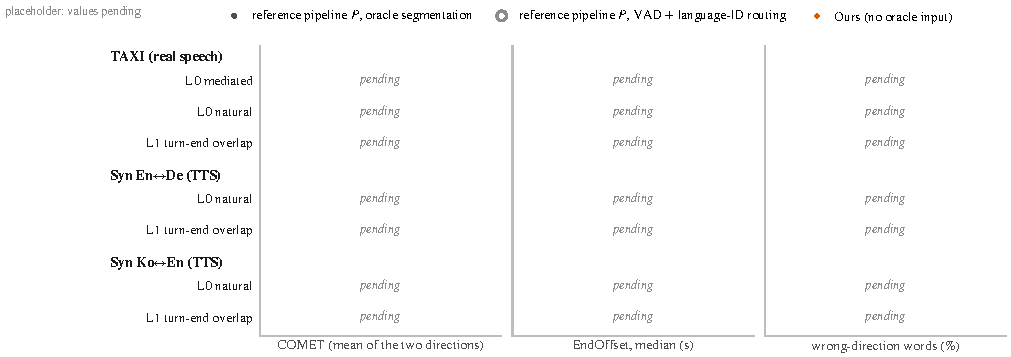
\includegraphics{figures/fig5_oracle_gap.pdf}
  \caption{Where the conversational difficulty lies (values pending; numbers will be in \cref{tab:conditions}). For each timing condition and language pair: the reference pipeline $P$ with oracle turn segmentation (filled) and with VAD and language-ID routing (hollow), and \model (diamond; no oracle input). $P$ covers both directions and has the highest realistic-wrapper COMET on \taxi L0 natural at its main operating point (\cref{sec:exp-setup}); it serves every row and both wrappers. Panels: COMET (mean of the two directions), median \eo and wrong-direction words. Rows are compared only through their gaps, not through absolute COMET.}
  \label{fig:gap}
\end{figure}

\paragraph{Full grid.}
For every timing condition, language pair and direction, \cref{tab:conditions} lists the systems run under it, each at its main operating point, fixed before the test runs; part~(a) also repeats every row of \cref{tab:main}, so that each has its interval. The offline systems receive gold turns and translate each turn after it ends. Their \laal therefore equals the mean source-turn duration (4.624\,s for \ende and 3.086\,s for \deen on \taxi), and their \eo is 0 on the ideal clock because their output is time-stamped at the gold turn end; \cref{tab:ca-latency} adds their compute. The gold-transcript row isolates translation quality, the Qwen3-ASR row adds the recognition of telephone-band speech, and Whisper ST covers \deen only. Under L1, an oracle segment cut from the mono mix also contains the overlapping speech of the other speaker; the oracle-separation row of \cref{tab:factorial} removes it. On \syn we interpret only rankings and effects relative to each pair's own offline systems with oracle input, never absolute scores across pairs.

% =====================================================================
% Table A5 (tab:conditions): full per-direction grid, the numbers behind
% Fig. 5 (fig:gap) and Fig. A3 (fig:gap-sweep). Included from App. E.
% Two floats: the second continues the first (\ContinuedFloat, caption package,
% keeps the table number; it has no label of its own).
% Known now: only the offline TAXI L0 natural rows (preliminary; the same runs
% as Table 3 / tab:main). Every other cell is pending (\tbd = blank).
% Row sets follow the experiment plan: CST-Bench-Syn runs the offline bounds,
% the three main pipelines and the model; SeamlessM4T v2 + AlignAtt runs on TAXI.
% The optional L1b stress test (not in v1) would add its own block and a
% backchannel-leakage column. When filling cells, keep the block structure.
% =====================================================================
\begin{table}[!tp]
  \caption{Full results by timing condition and language pair: the numbers behind \cref{fig:gap,fig:gap-sweep} (ideal clock; each system at its pre-registered main operating point). Part~(a) covers \taxi; parts~(b) and~(c) follow. Seg.: oracle = gold turns and source language; realistic = VAD and language-ID routing; none = the system segments the stream itself. Offline: gold$\to$LLM and ASR$\to$LLM translate the gold or the Qwen3-ASR-1.7B transcript of each turn with Qwen3.8-27B, and Whisper ST is Whisper-large-v3 translating into English; streaming cascade: streaming ASR and Qwen3.8-27B with LocalAgreement-2; M4T v2: SeamlessM4T v2 (\cref{tab:baselines}). X is German on \taxi and \syn \pair{En}{De}, and Korean on \syn \pair{Ko}{En}. Latencies are in seconds over non-empty turns: mean \laal and median \eo per direction; wrong-direction words, median switch latency and empty turns are pooled over both directions; \cref{tab:ca-latency} lists each system's encoder look-ahead $\ell_{\mathrm{enc}}$. Each estimate will carry the half-width of its 95\% session-clustered bootstrap CI as a subscript. Offline systems translate each oracle turn after it ends, so their \laal equals the mean source-turn duration and their \eo is 0 by construction. $^\dagger$preliminary; to be re-run under the final protocol (same runs as \cref{tab:main}; no CIs yet). --: not applicable; blank: pending. \protect\draftnote{L1 is not rendered yet}}
  \label{tab:conditions}
  \centering
  \footnotesize
  \setlength{\tabcolsep}{3pt}
  \begin{tabular}{@{}llccccccccccc@{}}
    \toprule
    & & \multicolumn{4}{c}{\dir{En}{X}} & \multicolumn{4}{c}{\dir{X}{En}} & \multicolumn{3}{c}{Both directions} \\
    \cmidrule(lr){3-6}\cmidrule(lr){7-10}\cmidrule(l){11-13}
    System & Seg. & COMET & chrF & \makecell{Stream-\\LAAL} & \makecell{End-\\Offset} & COMET & chrF & \makecell{Stream-\\LAAL} & \makecell{End-\\Offset} & \makecell{Wrong\\dir.\ (\%)} & \makecell{Switch\\latency} & \makecell{Empty\\turns (\%)} \\
    \midrule
    \multicolumn{13}{@{}l}{\textit{(a) \taxi, L0 natural}} \\
    Offline: gold$\to$LLM & oracle & \tbd & \prelim{71.72} & \prelim{4.62} & 0 & \tbd & \prelim{58.05} & \prelim{3.09} & 0 & \tbd & \tbd & \tbd \\
    Offline: ASR$\to$LLM & oracle & \tbd & \prelim{67.97} & \prelim{4.62} & 0 & \tbd & \prelim{56.61} & \prelim{3.09} & 0 & \tbd & \tbd & \tbd \\
    Offline: Whisper ST & oracle & -- & -- & -- & -- & \tbd & \prelim{56.67} & \prelim{3.09} & 0 & \tbd & \tbd & \tbd \\
    Consecutive cascade & realistic & \tbd & \tbd & \tbd & \tbd & \tbd & \tbd & \tbd & \tbd & \tbd & \tbd & \tbd \\
    SeamlessStreaming & oracle & \tbd & \tbd & \tbd & \tbd & \tbd & \tbd & \tbd & \tbd & \tbd & \tbd & \tbd \\
    SeamlessStreaming & realistic & \tbd & \tbd & \tbd & \tbd & \tbd & \tbd & \tbd & \tbd & \tbd & \tbd & \tbd \\
    Streaming cascade & oracle & \tbd & \tbd & \tbd & \tbd & \tbd & \tbd & \tbd & \tbd & \tbd & \tbd & \tbd \\
    Streaming cascade & realistic & \tbd & \tbd & \tbd & \tbd & \tbd & \tbd & \tbd & \tbd & \tbd & \tbd & \tbd \\
    M4T v2 + AlignAtt & oracle & \tbd & \tbd & \tbd & \tbd & \tbd & \tbd & \tbd & \tbd & \tbd & \tbd & \tbd \\
    M4T v2 + AlignAtt & realistic & \tbd & \tbd & \tbd & \tbd & \tbd & \tbd & \tbd & \tbd & \tbd & \tbd & \tbd \\
    \model & none & \tbd & \tbd & \tbd & \tbd & \tbd & \tbd & \tbd & \tbd & \tbd & \tbd & \tbd \\
    \midrule
    \multicolumn{13}{@{}l}{\textit{\taxi, L0 mediated}} \\
    Offline: gold$\to$LLM & oracle & \tbd & \tbd & \tbd & \tbd & \tbd & \tbd & \tbd & \tbd & \tbd & \tbd & \tbd \\
    Offline: ASR$\to$LLM & oracle & \tbd & \tbd & \tbd & \tbd & \tbd & \tbd & \tbd & \tbd & \tbd & \tbd & \tbd \\
    Offline: Whisper ST & oracle & -- & -- & -- & -- & \tbd & \tbd & \tbd & \tbd & \tbd & \tbd & \tbd \\
    Consecutive cascade & realistic & \tbd & \tbd & \tbd & \tbd & \tbd & \tbd & \tbd & \tbd & \tbd & \tbd & \tbd \\
    SeamlessStreaming & oracle & \tbd & \tbd & \tbd & \tbd & \tbd & \tbd & \tbd & \tbd & \tbd & \tbd & \tbd \\
    SeamlessStreaming & realistic & \tbd & \tbd & \tbd & \tbd & \tbd & \tbd & \tbd & \tbd & \tbd & \tbd & \tbd \\
    Streaming cascade & oracle & \tbd & \tbd & \tbd & \tbd & \tbd & \tbd & \tbd & \tbd & \tbd & \tbd & \tbd \\
    Streaming cascade & realistic & \tbd & \tbd & \tbd & \tbd & \tbd & \tbd & \tbd & \tbd & \tbd & \tbd & \tbd \\
    M4T v2 + AlignAtt & oracle & \tbd & \tbd & \tbd & \tbd & \tbd & \tbd & \tbd & \tbd & \tbd & \tbd & \tbd \\
    M4T v2 + AlignAtt & realistic & \tbd & \tbd & \tbd & \tbd & \tbd & \tbd & \tbd & \tbd & \tbd & \tbd & \tbd \\
    \model & none & \tbd & \tbd & \tbd & \tbd & \tbd & \tbd & \tbd & \tbd & \tbd & \tbd & \tbd \\
    \midrule
    \multicolumn{13}{@{}l}{\textit{\taxi, L1 (turn-end overlap)}} \\
    Offline: gold$\to$LLM & oracle & \tbd & \tbd & \tbd & \tbd & \tbd & \tbd & \tbd & \tbd & \tbd & \tbd & \tbd \\
    Offline: ASR$\to$LLM & oracle & \tbd & \tbd & \tbd & \tbd & \tbd & \tbd & \tbd & \tbd & \tbd & \tbd & \tbd \\
    Offline: Whisper ST & oracle & -- & -- & -- & -- & \tbd & \tbd & \tbd & \tbd & \tbd & \tbd & \tbd \\
    Consecutive cascade & realistic & \tbd & \tbd & \tbd & \tbd & \tbd & \tbd & \tbd & \tbd & \tbd & \tbd & \tbd \\
    SeamlessStreaming & oracle & \tbd & \tbd & \tbd & \tbd & \tbd & \tbd & \tbd & \tbd & \tbd & \tbd & \tbd \\
    SeamlessStreaming & realistic & \tbd & \tbd & \tbd & \tbd & \tbd & \tbd & \tbd & \tbd & \tbd & \tbd & \tbd \\
    Streaming cascade & oracle & \tbd & \tbd & \tbd & \tbd & \tbd & \tbd & \tbd & \tbd & \tbd & \tbd & \tbd \\
    Streaming cascade & realistic & \tbd & \tbd & \tbd & \tbd & \tbd & \tbd & \tbd & \tbd & \tbd & \tbd & \tbd \\
    M4T v2 + AlignAtt & oracle & \tbd & \tbd & \tbd & \tbd & \tbd & \tbd & \tbd & \tbd & \tbd & \tbd & \tbd \\
    M4T v2 + AlignAtt & realistic & \tbd & \tbd & \tbd & \tbd & \tbd & \tbd & \tbd & \tbd & \tbd & \tbd & \tbd \\
    \model & none & \tbd & \tbd & \tbd & \tbd & \tbd & \tbd & \tbd & \tbd & \tbd & \tbd & \tbd \\
    \bottomrule
  \end{tabular}
\end{table}

\begin{table}[!tp]
  \ContinuedFloat
  \caption[]{(continued) Part~(b): \syn, with the columns and conventions of part~(a). Part~(c): \taxi re-rendered with one fixed gap at every speaker change (a negative gap starts the next turn before the previous one ends), the numbers behind \cref{fig:gap-sweep}; COMET is the mean of the two directions, \eo the median over both directions, and the best pipeline is that of \cref{tab:factorial}. If the optional L1b stress test is adopted, it adds a block with a backchannel-leakage column. Blank: pending. \protect\draftnote{\syn and the fixed-gap renders are planned}}
  \centering
  \footnotesize
  \setlength{\tabcolsep}{3pt}
  \begin{tabular}{@{}llccccccccccc@{}}
    \toprule
    & & \multicolumn{4}{c}{\dir{En}{X}} & \multicolumn{4}{c}{\dir{X}{En}} & \multicolumn{3}{c}{Both directions} \\
    \cmidrule(lr){3-6}\cmidrule(lr){7-10}\cmidrule(l){11-13}
    System & Seg. & COMET & chrF & \makecell{Stream-\\LAAL} & \makecell{End-\\Offset} & COMET & chrF & \makecell{Stream-\\LAAL} & \makecell{End-\\Offset} & \makecell{Wrong\\dir.\ (\%)} & \makecell{Switch\\latency} & \makecell{Empty\\turns (\%)} \\
    \midrule
    \multicolumn{13}{@{}l}{\textit{(b) \syn \pair{En}{De}, L0 natural}} \\
    Offline: gold$\to$LLM & oracle & \tbd & \tbd & \tbd & \tbd & \tbd & \tbd & \tbd & \tbd & \tbd & \tbd & \tbd \\
    Offline: ASR$\to$LLM & oracle & \tbd & \tbd & \tbd & \tbd & \tbd & \tbd & \tbd & \tbd & \tbd & \tbd & \tbd \\
    Consecutive cascade & realistic & \tbd & \tbd & \tbd & \tbd & \tbd & \tbd & \tbd & \tbd & \tbd & \tbd & \tbd \\
    SeamlessStreaming & oracle & \tbd & \tbd & \tbd & \tbd & \tbd & \tbd & \tbd & \tbd & \tbd & \tbd & \tbd \\
    SeamlessStreaming & realistic & \tbd & \tbd & \tbd & \tbd & \tbd & \tbd & \tbd & \tbd & \tbd & \tbd & \tbd \\
    Streaming cascade & oracle & \tbd & \tbd & \tbd & \tbd & \tbd & \tbd & \tbd & \tbd & \tbd & \tbd & \tbd \\
    Streaming cascade & realistic & \tbd & \tbd & \tbd & \tbd & \tbd & \tbd & \tbd & \tbd & \tbd & \tbd & \tbd \\
    \model & none & \tbd & \tbd & \tbd & \tbd & \tbd & \tbd & \tbd & \tbd & \tbd & \tbd & \tbd \\
    \midrule
    \multicolumn{13}{@{}l}{\textit{\syn \pair{En}{De}, L1 (turn-end overlap)}} \\
    Offline: gold$\to$LLM & oracle & \tbd & \tbd & \tbd & \tbd & \tbd & \tbd & \tbd & \tbd & \tbd & \tbd & \tbd \\
    Offline: ASR$\to$LLM & oracle & \tbd & \tbd & \tbd & \tbd & \tbd & \tbd & \tbd & \tbd & \tbd & \tbd & \tbd \\
    Consecutive cascade & realistic & \tbd & \tbd & \tbd & \tbd & \tbd & \tbd & \tbd & \tbd & \tbd & \tbd & \tbd \\
    SeamlessStreaming & oracle & \tbd & \tbd & \tbd & \tbd & \tbd & \tbd & \tbd & \tbd & \tbd & \tbd & \tbd \\
    SeamlessStreaming & realistic & \tbd & \tbd & \tbd & \tbd & \tbd & \tbd & \tbd & \tbd & \tbd & \tbd & \tbd \\
    Streaming cascade & oracle & \tbd & \tbd & \tbd & \tbd & \tbd & \tbd & \tbd & \tbd & \tbd & \tbd & \tbd \\
    Streaming cascade & realistic & \tbd & \tbd & \tbd & \tbd & \tbd & \tbd & \tbd & \tbd & \tbd & \tbd & \tbd \\
    \model & none & \tbd & \tbd & \tbd & \tbd & \tbd & \tbd & \tbd & \tbd & \tbd & \tbd & \tbd \\
    \midrule
    \multicolumn{13}{@{}l}{\textit{\syn \pair{Ko}{En}, L0 natural}} \\
    Offline: gold$\to$LLM & oracle & \tbd & \tbd & \tbd & \tbd & \tbd & \tbd & \tbd & \tbd & \tbd & \tbd & \tbd \\
    Offline: ASR$\to$LLM & oracle & \tbd & \tbd & \tbd & \tbd & \tbd & \tbd & \tbd & \tbd & \tbd & \tbd & \tbd \\
    Consecutive cascade & realistic & \tbd & \tbd & \tbd & \tbd & \tbd & \tbd & \tbd & \tbd & \tbd & \tbd & \tbd \\
    SeamlessStreaming & oracle & \tbd & \tbd & \tbd & \tbd & \tbd & \tbd & \tbd & \tbd & \tbd & \tbd & \tbd \\
    SeamlessStreaming & realistic & \tbd & \tbd & \tbd & \tbd & \tbd & \tbd & \tbd & \tbd & \tbd & \tbd & \tbd \\
    Streaming cascade & oracle & \tbd & \tbd & \tbd & \tbd & \tbd & \tbd & \tbd & \tbd & \tbd & \tbd & \tbd \\
    Streaming cascade & realistic & \tbd & \tbd & \tbd & \tbd & \tbd & \tbd & \tbd & \tbd & \tbd & \tbd & \tbd \\
    \model & none & \tbd & \tbd & \tbd & \tbd & \tbd & \tbd & \tbd & \tbd & \tbd & \tbd & \tbd \\
    \midrule
    \multicolumn{13}{@{}l}{\textit{\syn \pair{Ko}{En}, L1 (turn-end overlap)}} \\
    Offline: gold$\to$LLM & oracle & \tbd & \tbd & \tbd & \tbd & \tbd & \tbd & \tbd & \tbd & \tbd & \tbd & \tbd \\
    Offline: ASR$\to$LLM & oracle & \tbd & \tbd & \tbd & \tbd & \tbd & \tbd & \tbd & \tbd & \tbd & \tbd & \tbd \\
    Consecutive cascade & realistic & \tbd & \tbd & \tbd & \tbd & \tbd & \tbd & \tbd & \tbd & \tbd & \tbd & \tbd \\
    SeamlessStreaming & oracle & \tbd & \tbd & \tbd & \tbd & \tbd & \tbd & \tbd & \tbd & \tbd & \tbd & \tbd \\
    SeamlessStreaming & realistic & \tbd & \tbd & \tbd & \tbd & \tbd & \tbd & \tbd & \tbd & \tbd & \tbd & \tbd \\
    Streaming cascade & oracle & \tbd & \tbd & \tbd & \tbd & \tbd & \tbd & \tbd & \tbd & \tbd & \tbd & \tbd \\
    Streaming cascade & realistic & \tbd & \tbd & \tbd & \tbd & \tbd & \tbd & \tbd & \tbd & \tbd & \tbd & \tbd \\
    \model & none & \tbd & \tbd & \tbd & \tbd & \tbd & \tbd & \tbd & \tbd & \tbd & \tbd & \tbd \\
    \bottomrule
  \end{tabular}

  \vspace{1.2em}
  \begin{tabular}{@{}lccccccccc@{}}
    \toprule
    & \multicolumn{3}{c}{Best pipeline, oracle} & \multicolumn{3}{c}{Best pipeline, realistic} & \multicolumn{3}{c}{\model} \\
    \cmidrule(lr){2-4}\cmidrule(lr){5-7}\cmidrule(l){8-10}
    Gap (s) & COMET & \makecell{Wrong\\dir.\ (\%)} & \makecell{End-\\Offset (s)} & COMET & \makecell{Wrong\\dir.\ (\%)} & \makecell{End-\\Offset (s)} & COMET & \makecell{Wrong\\dir.\ (\%)} & \makecell{End-\\Offset (s)} \\
    \midrule
    \multicolumn{10}{@{}l}{\textit{(c) \taxi, one fixed gap at every speaker change}} \\
    $-0.6$ & \tbd & \tbd & \tbd & \tbd & \tbd & \tbd & \tbd & \tbd & \tbd \\
    $-0.4$ & \tbd & \tbd & \tbd & \tbd & \tbd & \tbd & \tbd & \tbd & \tbd \\
    $-0.2$ & \tbd & \tbd & \tbd & \tbd & \tbd & \tbd & \tbd & \tbd & \tbd \\
    $0.05$ & \tbd & \tbd & \tbd & \tbd & \tbd & \tbd & \tbd & \tbd & \tbd \\
    $0.2$ & \tbd & \tbd & \tbd & \tbd & \tbd & \tbd & \tbd & \tbd & \tbd \\
    $0.5$ & \tbd & \tbd & \tbd & \tbd & \tbd & \tbd & \tbd & \tbd & \tbd \\
    $1.0$ & \tbd & \tbd & \tbd & \tbd & \tbd & \tbd & \tbd & \tbd & \tbd \\
    $2.0$ & \tbd & \tbd & \tbd & \tbd & \tbd & \tbd & \tbd & \tbd & \tbd \\
    \bottomrule
  \end{tabular}
\end{table}


\paragraph{Decomposing the gap.}
Let $Q_{TL}$ be the COMET of the row of \cref{tab:factorial} with gold turns ($T{=}1$) or VAD segments ($T{=}0$) and with the gold ($L{=}1$) or the identified ($L{=}0$) source language, so that the oracle gap of \cref{sec:exp-setup} is $G=Q_{11}-Q_{00}$. The segmentation effect
\begin{equation*}
  E_T=\tfrac12\bigl[(Q_{11}-Q_{01})+(Q_{10}-Q_{00})\bigr]
\end{equation*}
and the routing effect $E_L=\tfrac12[(Q_{11}-Q_{10})+(Q_{01}-Q_{00})]$ each average the loss from replacing one oracle component over both settings of the other component. They sum to $G$, which makes them the Shapley attribution for two factors, and the interaction $I=Q_{11}-Q_{10}-Q_{01}+Q_{00}$ measures how far the two losses compound. We report $E_T$, $E_L$ and $I$ in COMET points with session-bootstrap CIs, not as shares of $G$, which are unstable when $G$ is small. Repeating the factorial for the second-best pipeline (\tbdtext{}) gives $E_T$ and $E_L$ of \tbdtext{} and \tbdtext{} COMET under L1.

\paragraph{Gap dose-response.}
Each timing condition draws its gaps from one distribution. To test whether pipelines degrade smoothly as turns follow each other more closely, we re-render \taxi with one fixed gap $g$ at every speaker change, $g\in\{-0.6,-0.4,-0.2,0.05,0.2,0.5,1.0,2.0\}$\,s, each rendering under its own configuration name and checksums; a negative gap starts the next turn $|g|$ before the previous one ends, as in L1. We run $P$ with both wrappers, and \model (\cref{fig:gap-sweep}; numbers in part~(c) of \cref{tab:conditions}). A smooth trend would show that the conclusions do not hinge on the chosen L0 and L1 distributions; a sharp drop would locate the gap at which VAD-based routing breaks down. From $g=2$\,s to $g=-0.6$\,s, COMET changes by \tbdtext{} with the realistic wrapper, by \tbdtext{} with oracle segmentation and by \tbdtext{} for \model.

\begin{figure}[t]
  \centering
  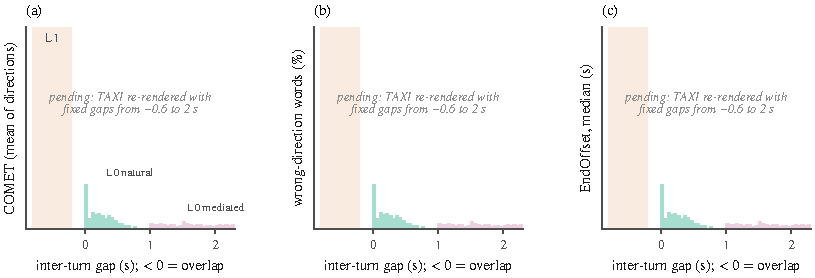
\includegraphics{figures/figA3_gap_sweep.pdf}
  \caption{Gap dose-response: \taxi re-rendered with one fixed gap at every speaker change, from $-0.6$\,s (overlap) to 2\,s. (a)~COMET (mean of the two directions), (b)~wrong-direction words and (c)~median \eo for the reference pipeline $P$ (solid: oracle segmentation; dashed: VAD and language-ID routing) and \model. Background histograms show the gaps drawn at the 540 speaker changes under L0 natural (green) and L0 mediated (pink); the shaded band is the overlap range of L1, whose next turn starts 0.2--0.8\,s before the previous one ends. Numbers in part~(c) of \cref{tab:conditions}. \protect\draftnote{results pending; the fixed-gap renders are planned}}
  \label{fig:gap-sweep}
\end{figure}

\paragraph{Why simultaneous? Latency by turn length.}
With oracle endpoints, offline systems reach an \eo of 0 on the ideal clock, which raises the question of why simultaneity is needed at all. A deployed consecutive system must first detect that a turn has ended, so the listener waits for the endpoint detector and, on the computation-aware clock, also for the translation of the whole turn. Lag within a turn grows with the turn as well: a system that emits a turn's translation only after the turn ends scores a \laal of at least the turn's duration (\cref{sec:bench}). \taxi turns are short (median 2.86\,s), but 22.5\% of them exceed 5\,s (\cref{tab:taxi-full}). \Cref{fig:turn-length} therefore breaks median \eo and \laal down by source-turn duration for the realistic consecutive cascade, the best realistic streaming pipeline and \model. For turns longer than 6\,s, the median \eo is \tbdtext{}\,s for the consecutive cascade, \tbdtext{}\,s for the best streaming pipeline and \tbdtext{}\,s for \model.

\begin{figure}[t]
  \centering
  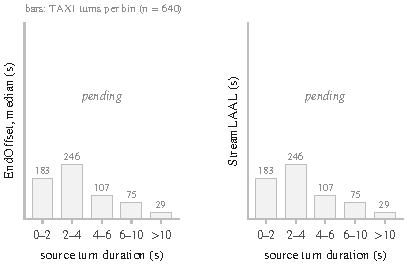
\includegraphics{figures/figA5_turn_length.pdf}
  \caption{Why simultaneous? Median \eo (left) and \laal (right) by source-turn duration on \taxi L0 natural, for the realistic consecutive cascade, the best realistic streaming pipeline and \model. Bars: \taxi turns per duration bin (183, 246, 107, 75 and 29 of 640). \protect\draftnote{results pending}}
  \label{fig:turn-length}
\end{figure}

\paragraph{Computation-aware latency.}
Main-text latencies use the ideal clock. \Cref{tab:ca-latency} times every system on one H200 GPU, as a single stream without batching, and re-scores it on the computation-aware clock, on which an emission time also counts the processing time spent until the emission \citep{ma2020simulmt}. It includes the three controls of \cref{tab:ablation}, because the ideal clock hides how much their compute differs from \model's: the same-backbone cascade, for instance, re-translates the growing transcript with a 27B LLM after every update. Streaming systems receive the audio in 80\,ms chunks; we report the median and the 99th percentile of the processing time per chunk (tick) and the real-time factor (RTF). Consecutive and offline systems are timed per turn. The only timings so far were taken outside this protocol. The single-speaker backbone with the 0.6B thinker takes about 60\,ms per chunk at the median on an H200 but 100--150\,ms at the 99th percentile, so it misses the 80\,ms budget there; on an M4 Mac with the thinker in MLX (fp16), it takes 56\,ms per chunk at the median and runs at an RTF of 0.82. In the preliminary offline run, batched compute moved the median \eo of the offline systems from 0 to at most about \prelim{0.2}\,s ($^\dagger$preliminary; to be re-run under the final protocol). The 1.7B thinker has not been timed, and we claim real time only for a system with a measured RTF below 1.

% =====================================================================
% Table A6 (tab:ca-latency): computation-aware latency and real-time factor.
% Included from App. E. Referenced from Secs. 4, 5, 6 and 7.
% Known now: (i) context rows = earlier measurements of the single-speaker
% 0.6B backbone (H200: tick p50 about 60 ms, p99 100-150 ms; M4 Mac with an
% MLX fp16 thinker: 56 ms p50, RTF 0.82), taken outside this protocol;
% (ii) the EndOffset of the three offline systems with measured, batched
% compute from the preliminary offline run: at most about 0.2 s (gold/ASR ->
% LLM 0.1-0.2 s, Whisper ST lower; approximate; quoted only as "<= 0.2");
% (iii) values that hold by construction (offline EndOffset 0 on the ideal
% clock; l_enc = 80 ms, the bound of the [56,0] encoder, also for M1-based
% controls). The 1.7B thinker has not been timed. The controls of Table 6
% (tab:ablation) are listed because their compute differs most from the
% model's. Everything else is pending (\tbd = blank).
% =====================================================================
\begin{table}[t]
  \caption{Computation-aware latency and real-time factor (RTF) on one H200 GPU, single stream, no batching; \taxi L0 natural, pooled over both directions. $\ell_{\mathrm{enc}}$: encoder look-ahead, counted at its bound. Tick: processing time per 80\,ms input chunk; RTF: processing time over audio duration. A real-time claim needs a measured RTF below 1; a tick above 80\,ms means that the output falls behind the input for a while. Ideal clock: an emission time is the audio consumed; computation-aware (CA) clock: it also counts the processing time spent until the emission \citep{ma2020simulmt}. \laal is a mean and \eo a median over non-empty turns. The batched offline row covers the three offline systems of the preliminary offline run, with approximate compute; the context rows are earlier measurements of the single-speaker backbone with the 0.6B thinker (not a \task system), taken outside this protocol. $^\dagger$preliminary; to be re-run under the final protocol. --: not applicable or not reported; blank: pending. \protect\draftnote{planned except the batched offline row and the context rows}}
  \label{tab:ca-latency}
  \centering
  \footnotesize
  \setlength{\tabcolsep}{4pt}
  \begin{tabular}{@{}llcccccccc@{}}
    \toprule
    & & & \multicolumn{2}{c}{Tick (ms)} & & \multicolumn{2}{c}{\laal (s)} & \multicolumn{2}{c}{\eo (s)} \\
    \cmidrule(lr){4-5}\cmidrule(lr){7-8}\cmidrule(l){9-10}
    System & Hardware & $\ell_{\mathrm{enc}}$ (ms) & p50 & p99 & RTF & ideal & CA & ideal & CA \\
    \midrule
    \model (1.7B thinker)              & H200 & 80   & \tbd & \tbd & \tbd & \tbd & \tbd & \tbd & \tbd \\
    SeamlessStreaming                  & H200 & \tbd & \tbd & \tbd & \tbd & \tbd & \tbd & \tbd & \tbd \\
    Streaming cascade                  & H200 & \tbd & \tbd & \tbd & \tbd & \tbd & \tbd & \tbd & \tbd \\
    M4T v2 + AlignAtt                  & H200 & \tbd & \tbd & \tbd & \tbd & \tbd & \tbd & \tbd & \tbd \\
    Consecutive cascade (unbatched)    & H200 & --   & --   & --   & \tbd & \tbd & \tbd & \tbd & \tbd \\
    Offline: ASR$\to$LLM, per turn (unbatched) & H200 & -- & -- & -- & \tbd & \tbd & \tbd & 0 & \tbd \\
    Offline systems, batched           & --   & --   & --   & --   & --   & --   & --   & 0 & $\leq$\prelim{0.2} \\
    \midrule
    \multicolumn{10}{@{}l}{\textit{Controls of \cref{tab:ablation}}} \\
    Decoupled twin                     & H200 & 80   & \tbd & \tbd & \tbd & \tbd & \tbd & \tbd & \tbd \\
    Same-backbone cascade (M1$\to$LLM) & H200 & 80   & \tbd & \tbd & \tbd & \tbd & \tbd & \tbd & \tbd \\
    Size-matched cascade (ASR$\to$1.7B LLM) & H200 & \tbd & \tbd & \tbd & \tbd & \tbd & \tbd & \tbd & \tbd \\
    \midrule
    \multicolumn{10}{@{}l}{\textit{Context: single-speaker ASR backbone, 0.6B thinker (not a \task system)}} \\
    0.6B backbone                      & H200   & 80 & $\approx$60 & 100--150 & --   & -- & -- & -- & -- \\
    0.6B backbone, MLX fp16 thinker    & M4 Mac & 80 & 56          & --       & 0.82 & -- & -- & -- & -- \\
    \bottomrule
  \end{tabular}
\end{table}


\paragraph{Failure taxonomy.}
\Cref{tab:failures} counts six failure types per 100 source turns; short turns are a particular risk, as 59 \taxi turns have at most three words. The detectors work on the scorer's alignments and timelines, so the table reports counts without showing any TAXI text, and their thresholds are fixed before the test runs. Merged turns, in which one VAD segment or output piece spans turns of both speakers, send one speaker's words to the wrong channel or delay the switch. A truncated tail leaves the last words of a turn untranslated, for example when a segment is closed early. Hallucinations are output words without an aligned reference word and with low reference-free quality \citep{rei2022cometkiwi}, cross-checked against the critical-error spans of xCOMET \citep{guerreiro2024xcomet}. We estimate the precision of each detector by hand on 50 \syn turns per condition, and any example we show comes from \syn. Under L1, $P$ with the realistic wrapper merges \tbdtext{} turns per 100 (L0 natural: \tbdtext{}), and \model merges \tbdtext{}.

% =====================================================================
% Table A8 (tab:failures): failure taxonomy. Included from App. E.
% Nothing is measured yet: every count cell is pending (\tbd = blank).
% Detectors run on the scorer's alignments and timelines, so the table shows
% counts only; detector thresholds are fixed before the test runs.
% Manual precision checks and any examples use CST-Bench-Syn only (no TAXI
% text may appear). The optional L1b stress test would add a row for
% translated backchannels.
% =====================================================================
\begin{table}[htbp]
  \caption{Failure taxonomy: counts per 100 source turns on \taxi L0 natural (L0) and L1, found by automatic detectors on the scorer's alignments; pipelines run with the realistic wrapper. Each detector's precision is checked by hand on 50 \syn turns per condition, never on TAXI text. Consec.: consecutive cascade; Seamless: SeamlessStreaming; Stream.\ casc.: streaming cascade; M4T+AA: M4T v2 + AlignAtt. Thresholds are fixed before the test runs. Blank: pending. \protect\draftnote{planned; if the optional L1b stress test is adopted, a row for translated backchannels is added}}
  \label{tab:failures}
  \centering
  \footnotesize
  \setlength{\tabcolsep}{3.5pt}
  \begin{tabular}{@{}>{\raggedright\arraybackslash}p{2.3cm}>{\raggedright\arraybackslash}p{6.2cm}cccccccccc@{}}
    \toprule
    & & \multicolumn{2}{c}{Consec.} & \multicolumn{2}{c}{Seamless} & \multicolumn{2}{c}{\makecell{Stream.\\casc.}} & \multicolumn{2}{c}{M4T+AA} & \multicolumn{2}{c}{\model} \\
    \cmidrule(lr){3-4}\cmidrule(lr){5-6}\cmidrule(lr){7-8}\cmidrule(lr){9-10}\cmidrule(l){11-12}
    Failure type & Detector & L0 & L1 & L0 & L1 & L0 & L1 & L0 & L1 & L0 & L1 \\
    \midrule
    Merged turns       & One VAD segment, or one output piece, spans turns of both speakers & \tbd & \tbd & \tbd & \tbd & \tbd & \tbd & \tbd & \tbd & \tbd & \tbd \\
    Wrong direction    & Words on the wrong channel for the active turn, in the wrong language, or copied from the source (scorer detector) & \tbd & \tbd & \tbd & \tbd & \tbd & \tbd & \tbd & \tbd & \tbd & \tbd \\
    Truncated tail     & The final words of the turn's reference stay unaligned & \tbd & \tbd & \tbd & \tbd & \tbd & \tbd & \tbd & \tbd & \tbd & \tbd \\
    Empty turn         & No output word is assigned to the turn & \tbd & \tbd & \tbd & \tbd & \tbd & \tbd & \tbd & \tbd & \tbd & \tbd \\
    Hallucination      & Output with no aligned reference word and low reference-free QE \citep{rei2022cometkiwi}; xCOMET critical-error spans \citep{guerreiro2024xcomet} as a cross-check & \tbd & \tbd & \tbd & \tbd & \tbd & \tbd & \tbd & \tbd & \tbd & \tbd \\
    Late switch        & Switch latency above 2\,s & \tbd & \tbd & \tbd & \tbd & \tbd & \tbd & \tbd & \tbd & \tbd & \tbd \\
    \bottomrule
  \end{tabular}
\end{table}


\paragraph{Transcripts and speakers.}
\Cref{tab:aux} scores DER with a 0.25\,s collar. Without a collar, every boundary error counts at the 80\,ms resolution; DER on \taxi L0 natural is then \tbdtext{} for \model with $\delta_s=2$ and \tbdtext{} for the streaming diarization cascade, and \tbdtext{} and \tbdtext{} under L1. The time-constrained tcpWER of \cref{app:scorer} on \taxi L1 is \tbdtext{} for \model with $\delta_s=2$ and \tbdtext{} for the streaming diarization cascade. In this release each speaker keeps one language, so the language reveals the speaker and DER mostly measures boundary timing; speakers who switch languages, which we exclude, would break this equivalence.

\paragraph{Ablations.}
Every row of \cref{tab:ablation} starts from the same M1 checkpoint (\cref{sec:model-training}). The reference, \model (M3), commits translations at MU2 units, writes speaker tags, sees L1-like overlapping sessions in training and is conditioned on $\delta_t$ through its prefix (\cref{sec:model-stream}). Each ablation changes one of these: translations committed only at turn ends (the targets of M2), direction tags without speaker tags, training from M1 without L1-like sessions (optional), and one model per $\delta_t$ instead of the conditioning (optional). Without speaker tags, the stream still carries the direction tags, which reveal the speaker as long as each speaker keeps one language; this row therefore tests whether an explicit speaker channel helps translation, not whether coupling turn-taking and translation helps, which the decoupled twin and the same-backbone cascade test (\cref{sec:exp-ablation,app:baselines}). Rows of runs that are cut are removed, not left blank; the computation-aware latency of the three controls is in \cref{tab:ca-latency}.

% Flush this appendix's floats (Tables A6, A8) before App. F starts.
\clearpage

% =====================================================================
% Appendix F: model and backbone details (one-column appendix).
% Built: the streaming ASR backbone (Stages 0-1). Planned: everything specific
% to CST (speaker tags, translation streams, activity head, Stages 2-3).
% Floats: Table A11 (tables/tab_training), Fig. A7 (fig:delta-delay),
% Table A9 (tables/tab_backbone), Fig. A6 (fig:backbone).
% Every number here is single-speaker English/Korean transcription, not CST.
% Do not cite the three-epoch Stage-1 runs until their numbers are recorded.
% Holds the details moved out of Sec. 5 for the page limit: loss weights,
% delay medians (earlier 0.6B models), Stage-2/3 data recipes, per-speaker
% forced alignment before mixing, the decoupled twin (as in Sec. 6.6 and
% App. D), the caveat that the model and its M1-based controls, unlike the
% baselines, train on benchmark-like simulated sessions, the decoding cap,
% session length in audio positions, licences.
% Error-rate differences are written as signed numbers ("difference"), not
% with \Delta, which denotes the 80 ms chunk length in Sec. 5.
% =====================================================================
% \mdltok is defined in sections/05_model.tex; this fallback only matters if
% this file is compiled without that section.
\providecommand{\mdltok}[1]{\ensuremath{\langle\mathrm{#1}\rangle}}

\section{Model and Backbone Details}\label{app:model}

This appendix specifies the streaming backbone of \model, the only part that is built, and evaluates it on single-speaker English and Korean transcription; none of its numbers is a \task result. It also records the training recipes of the planned stages. \Cref{tab:training} lists the training stages, \cref{tab:backbone,fig:backbone} report the backbone, and \cref{fig:delta-delay} works through the delay rule of \cref{sec:model-backbone} on a recorded utterance.

\paragraph{Encoder.}
The encoder of Nemotron~3.5 ASR Streaming 0.6B \citep{nvidia2026nemotron35asr} is a cache-aware FastConformer \citep{gulati2020conformer,rekesh2023fast,noroozi2024stateful}: 128-bin log-mel features (25\,ms window, 10\,ms hop), depthwise-striding subsampling by 8 and 24 layers with $d_{\mathrm{model}}=1024$ and 8 heads, so one frame covers 80\,ms and a stream of $T$\,s yields $K=\mathrm{round}(12.5\,T)$ frames. Its attention context $[56,N]$ gives the number of 80\,ms frames visible to the left and to the right. We use $[56,0]$, i.e.\ 4.48\,s of left context and none on the right; the released checkpoint defaults to $[56,3]$, which adds 240\,ms of right context. With $[56,0]$, encoding a whole utterance at once yields the same frames as streaming, so training encodes each batch without a cache, and live inference uses the cache-aware step, whose output is frame-identical. The encoder's own RNN-T decoder \citep{graves2012sequence} serves only as a baseline (\cref{tab:backbone}). When the encoder is trained, its attention context is sampled per step from $[56,0]$, $[56,3]$, $[56,6]$ and $[56,13]$, so one checkpoint can be evaluated at several look-aheads (\cref{fig:backbone}).

\paragraph{Effective look-ahead.}
A nominal context can hide look-ahead, so we measure it. We encode a 14.84\,s LibriSpeech \citep{panayotov2015librispeech} utterance from its full features and from features truncated at 3, 6, 9 and 12\,s and compare the outputs frame by frame (fp32, TF32 disabled, relative tolerance $10^{-3}$); the effective look-ahead is the span before the cut in which the outputs differ. With $[56,0]$, only the last frame changes, through the boundary of the subsampling convolution, so the look-ahead is 80\,ms at every cut; with $[56,3]$, it is 160, 240 and 320\,ms (minimum, mean and maximum over the cuts). Two strictly causal reference models give 0\,ms, which validates the test. The test also shows why Qwen3-ASR's own audio encoder is removed: in the implementation we tested, its attention spans the whole utterance, and even its intended mode with 1\,s blocks looks ahead by 420\,ms on average and by up to 800\,ms.

\paragraph{Adapter and thinker.}
The adapter is LayerNorm, Linear ($1024\to2048$), GELU and Linear ($2048\to h$), where $h$ is the hidden size of the thinker: 1024 for the 0.6B thinker and 2048 for the 1.7B one (4.2M and 6.3M adapter parameters). The 0.6B thinker is a Qwen3 decoder with 28 layers, 16 query and 8 key-value heads of dimension 128, a feed-forward size of 3072, a vocabulary of 151,936 tokens and tied input and output embeddings. The adapter output replaces the input embedding at each audio placeholder position (token 151676), one per 80\,ms chunk. \model uses the 1.7B thinker, the language model of Qwen3-ASR-1.7B \citep{shi2026qwen3asr,xu2025qwen3omni}; the 0.6B thinker serves for pilots. With the 1.7B thinker, Stage~1 trains 2,336M parameters: thinker, encoder and adapter. The encoder is released under OpenMDW-1.1 and the thinker under Apache-2.0.

\paragraph{Sequence and special tokens.}
The input-only prefix follows the chat format of Qwen3-ASR with an empty system turn; the assistant turn opens with the line ``language English'' or ``language Korean'', the transcript marker and \mdltok{DELAY\_\delta}. The prefixes of the two languages differ only in that line, so the language is an input and the backbone performs no language identification. Each chunk $k$ then contributes $a_k$, the text tokens due in it and the end-of-chunk token \mdltok{next} (NEXT\_AUDIO in \cref{fig:delta-delay}), the analogue of a transducer blank \citep{graves2012sequence,seide2024speech}. After the last chunk, a flush round (\mdltok{empty}, the remaining text tokens, \mdltok{next}) runs if tokens remain, and a final round (\mdltok{empty}, \mdltok{next}) always runs; \mdltok{empty} (EMPTY\_AUDIO) is an input placeholder that carries no loss. Twelve special tokens use spare rows of the embedding matrix, so the vocabulary is not resized, and each is initialised as the mean embedding plus $0.02\,\mathcal{N}(0,1)$ noise: \mdltok{next} (id 151705), \mdltok{empty} (151706), the speaker tags \mdltok{A} and \mdltok{B} (151707 and 151708), which are reserved but untrained and blocked at decoding, and \mdltok{DELAY\_1} to \mdltok{DELAY\_8} (151709--151716). In the 0.6B model, token ids end at 151716 while the embedding matrix has 151,936 rows, which leaves 219 unused rows for the target-language tags and the translation delay tokens of \model, whose prefix (\cref{sec:model-stream}) names the language pair and carries \mdltok{DELAY\_\delta_s} and \mdltok{TDELAY\_\delta_t}. With one audio position per chunk, the longest \taxi session (90.02\,s) spans about 1.1k audio positions.
\draftnote{planned: these tags are not yet allocated}

\begin{figure}[t]
  \centering
  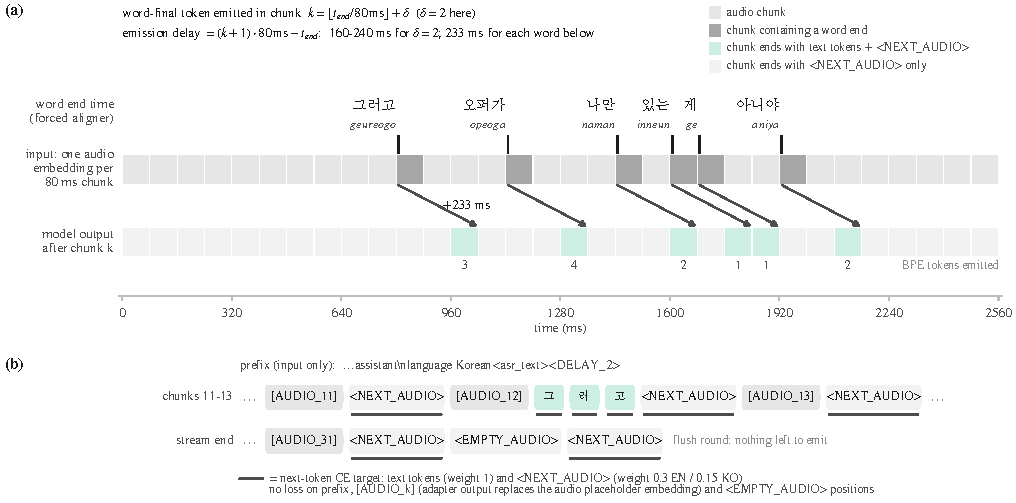
\includegraphics[width=\textwidth]{figures/figA7_delta_delay.pdf}
  \caption{Delay rule of the single-speaker backbone on a recorded KsponSpeech \citep{bang2020ksponspeech} utterance (2.6\,s, $K=32$ chunks, $\delta=2$). (a)~One audio embedding enters per 80\,ms chunk. A word that ends at $t_{\mathrm{end}}$ (forced alignment) is emitted, with all its BPE tokens, after chunk $k=\lfloor t_{\mathrm{end}}/80\,\mathrm{ms}\rfloor+\delta$, so its emission delay $(k+1)\cdot80\,\mathrm{ms}-t_{\mathrm{end}}$ lies between 160 and 240\,ms for $\delta=2$; here it is 233\,ms for all six words. Numbers under the output row count the BPE tokens emitted. (b)~Serialized LM sequence for chunks 11--13 and the end of the stream. Underlined tokens are next-token targets, weighted 1 for text and 0.3 (English) or 0.15 (Korean) for the end-of-chunk token \mdltok{next} (NEXT\_AUDIO); the prefix, the audio positions and \mdltok{empty} (EMPTY\_AUDIO) carry no loss.}
  \label{fig:delta-delay}
\end{figure}

\paragraph{Targets, loss and decoding.}
Targets are normalised lexical transcripts (lowercase, no punctuation, numbers spelled out). Word end times come from Qwen3-ForcedAligner \citep{shi2026qwen3asr} at 80\,ms resolution, and all tokens of a word are due in the chunk that the delay rule assigns to the word's end; tokens due at or after the last chunk go to the flush round, and tokens due in the same chunk keep their end-time order. Training imposes no limit on the tokens per chunk. On LibriSpeech and KsponSpeech, targets average 0.22 and 0.27 text tokens per chunk, and 75--80\% of the chunks emit only \mdltok{next}; \cref{eq:loss} therefore weights \mdltok{next} by 0.3 (English) or 0.15 (Korean) and every other label, including the planned tags, by 1. The output layer is computed only at labelled positions, which bounds memory on long sequences. Decoding is greedy with a KV cache, with one forward pass per chunk and one per emitted token; it forces \mdltok{next} after 8 tokens in a chunk or $6K+64$ tokens in a stream, runs flush rounds until one is empty (at most 8), and blocks the chat-format, audio, transcript-marker, \mdltok{empty}, speaker and delay tokens. Translation segments will need a higher per-chunk cap.\draftnote{planned} On one H200 GPU, decoding with the 0.6B thinker needs 100--150\,ms per 80\,ms chunk at the 99th percentile, so real time is not yet shown; the 1.7B thinker has not been timed (\cref{tab:ca-latency}). In earlier backbones with the 0.6B thinker, $\delta=2/3/4$ gave a median emission delay $(k+1)\cdot80\,\mathrm{ms}-t$ of about 200/280/360\,ms, which excludes the 80\,ms encoder look-ahead that \cref{sec:model-inference} adds, and at most 0.5\% of English emissions (2--5\% of Korean ones) came 80\,ms or more before their target chunk; the evaluation of the 1.7B pilot recorded no emission delays. \Cref{fig:delta-delay} shows the rule on a 2.6\,s utterance: its six words end at 807, 1127, 1447, 1607, 1687 and 1927\,ms and are emitted after chunks 12, 16, 20, 22, 23 and 26, each 233\,ms after its end; chunks 0--11 and 27--31 emit only \mdltok{next}, and the flush round is empty.

\paragraph{Training.}
Stage~0 trains only the adapter, with the thinker frozen, in final mode (the native Qwen3-ASR format), because a randomly initialised adapter otherwise causes very large gradients in the first steps. Stage~1 starts from Stage~0 and the original Qwen3-ASR thinker and trains all parts for one epoch, with $\delta\in\{2,3,4,6,8\}$ and final mode for each utterance with probability 0.3 (\cref{tab:training}). Its data are about 3.8k\,h drawn from a quality-controlled pool of 19 English and Korean sources, plus about 4.3k\,h of ASR corpora: 806\,h of English from LibriSpeech \citep{panayotov2015librispeech}, VoxPopuli \citep{wang2021voxpopuli}, Granary-YODAS \citep{koluguri2025granary} and Switchboard \citep{godfrey1992switchboard}, and about 3.5k\,h of Korean from KsponSpeech \citep{bang2020ksponspeech}, NIKL conversational speech and AI~Hub conversational and broadcast speech; there is no German. We augment with SpecAugment \citep{park2019specaugment} (2 frequency masks of up to 27 bins and 2 time masks of up to 3\% of the utterance), speed perturbation (0.9, 1.0, 1.1), noise (probability 0.4, SNR 5--30\,dB), music (SNR 10--30\,dB) and reverberation (probability 0.2). The noise bank holds 8.9\,h of noise (MUSAN, \citealp{snyder2015musan}; DEMAND, \citealp{thiemann2013demand}; ETSI), 42.6\,h of music (MUSAN) and 6,325 simulated and real room impulse responses; reverberation is applied before noise, and the direct-path peak of each impulse response is aligned to $t=0$ so that word times stay valid. Stronger time masking (about 12\% of the frames) lowered the top-1 accuracy on text tokens at the first step from 0.985 to 0.84, so we avoid it. One epoch takes 3,980 steps on 2 nodes with 8 GPUs each, at about 2.5\,s per step including I/O stalls (0.6--1.0\,s of compute); the training loss ended at 0.27 and was still falling. The 0.6B pilot uses the same data, steps and augmentation. After training, we reload each checkpoint and compare it with the model in memory key by key, encoder included; for both pilots no key differs, including all 638 encoder tensors.
\draftnote{longer Stage-1 runs exist but stay out of the paper until their numbers are recorded with a per-epoch analysis}

% =====================================================================
% Table A11 (tab:training): training stages. Included from App. F.
% Stages 0-1 exist (Stage 1 = the one-epoch pilot behind tab:backbone).
% Stages 2-3 are planned: their Data/Targets cells restate the design of
% Sec. 5 (sec:model); every setting that is still open is \tbd (blank).
% =====================================================================
\begin{table}[t]
  \caption{Training stages, data and hyperparameters. Stages~0 and~1 exist, and the one-epoch Stage-1 pilot is the backbone of \cref{tab:backbone}; Stages~2 and~3 are planned (M1--M3 as in \cref{sec:model}), and their open settings are blank. Hours are approximate; data sources and augmentation are detailed in \cref{app:model}. lr: peak learning rate after a linear warm-up.}
  \label{tab:training}
  \centering
  \footnotesize
  \setlength{\tabcolsep}{2.5pt}
  \renewcommand{\arraystretch}{1.1}
  \begin{tabular}{@{}>{\raggedright\arraybackslash}p{2.1cm}>{\raggedright\arraybackslash}p{1.9cm}>{\raggedright\arraybackslash}p{3.6cm}>{\raggedright\arraybackslash}p{2.9cm}>{\raggedright\arraybackslash}p{3.0cm}>{\raggedright\arraybackslash}p{1.35cm}>{\raggedright\arraybackslash}p{1.1cm}@{}}
    \toprule
    Stage & Trainable & Data & Targets & Schedule & Hardware & Status \\
    \midrule
    0: adapter warm-up
      & adapter (6.3M); thinker frozen
      & English and Korean ASR
      & final mode only (Qwen3-ASR format)
      & 2,000 steps, warm-up 100; 16,384-token batches
      & 1 node
      & built \\
    \addlinespace
    1: streaming and final-mode ASR
      & encoder, adapter, thinker (2,336M)
      & $\approx$3.8k\,h curated English and Korean speech + $\approx$4.3k\,h English and Korean ASR corpora (806\,h English); no German; augmented
      & lexical transcripts; $\delta\in\{2,3,4,6,8\}$; final mode with probability 0.3
      & 1 epoch = 3,980 steps; lr $6{\times}10^{-5}$ thinker (warm-up 500), $10^{-3}$ adapter, $10^{-5}$ encoder
      & 2 nodes $\times$ 8 GPUs
      & built (pilot) \\
    \addlinespace
    2 (M1): two-speaker bilingual ASR
      & \tbd
      & + German ASR, 8\,kHz telephone-band augmentation, simulated two-speaker \pair{En}{De} and \pair{En}{Ko} mono sessions
      & speaker-tagged transcripts at delay $\delta_s$; two-slot speaker activity
      & \tbd
      & \tbd
      & planned \\
    \addlinespace
    3 (M2, M3): translation streams
      & \tbd
      & + CoVoST~2 and MuST-C (\pair{En}{De}); silver teacher translations in four directions
      & translations committed at turn ends (M2) or at MU2 (M3), delay $\delta_t$
      & \tbd
      & \tbd
      & planned \\
    \bottomrule
  \end{tabular}
\end{table}


\paragraph{Planned stages.}
Stage~2 (M1) starts from the 1.7B Stage-1 pilot and adds German ASR data, 8\,kHz telephone-band augmentation, the speaker tags and the activity head, trained on simulated two-speaker \pair{En}{De} and \pair{Ko}{En} mono sessions whose gaps and overlaps are drawn more broadly than in the benchmark \citep[cf.][]{landini2022from}. Each speaker's turns are force-aligned before mixing, so that the words of both speakers can be ordered by end time under overlap (\cref{sec:model-stream}). Before training M1, we fixed three acceptance criteria: single-speaker WER and CER at most 5\% (relative) above those of the Stage-1 pilot on VoxPopuli-AA and KsponSpeech, cpWER on synthetic L0 sessions at most 1.2 times the matched single-speaker WER, and a speaker-attribution error of at most 5\%. Stage~3 then adds the translation streams of \cref{sec:model-targets}, committed at turn ends (M2) or at MU2 (M3), from human \pair{En}{De} speech translation data, CoVoST~2 \citep{wang2021covost} and MuST-C \citep{digangi2019must}, and from silver teacher translations in four directions. The same-backbone cascade and the decoupled twin of \cref{sec:exp-ablation} also start from M1 and train on the same data (\cref{app:baselines}). Unlike the off-the-shelf baselines, \model and both controls thus train on simulated sessions built like the benchmark's; the fixed-gap sweep (\cref{fig:gap-sweep}) tests whether gains depend on the benchmark's gap distribution. Training excludes \taxi, the dialogue corpora and voices of \syn, and outputs of EXAONE-4.0 \citep{lgai2025exaone4}, which serves only for evaluation (\cref{app:syn,app:units}).
\draftnote{planned; German data still has to be obtained, and if M1 misses the criteria twice, M1 transcripts translated by an LLM become our system}

\paragraph{Evaluation protocol.}
Backbone results use a single-turn protocol: each utterance is followed by 1\,s of digital silence, the state is reset per utterance, and decoding is greedy in fp32 with TF32 disabled. English is scored by WER and Korean by CER without spaces, after normalising the text with numbers spelled out. VoxPopuli-AA is a cleaned release of the VoxPopuli test set \citep{wang2021voxpopuli} (628 utterances, 1.98\,h, 292 sessions, 18,072 reference words); AA-WER approximates the scoring published with it, part of which is not public: we apply Whisper's text normalisation \citep{radford2023robust}, split digits and weight the mean by utterance duration. KsponSpeech \citep{bang2020ksponspeech} eval\_clean and eval\_other have 3,000 and 2,687 utterances. Paired bootstrap tests use 2,000 resamples, clustered by session on VoxPopuli-AA and by utterance on KsponSpeech; we call a difference significant if its 95\% interval excludes zero. Differences and relative changes are computed from unrounded error rates.

% =====================================================================
% Table A9 (tab:backbone): single-speaker streaming ASR backbone. Included from App. F.
% All values are measured on the single-turn protocol: the two one-epoch
% Stage-1 pilots, two earlier 0.6B models and two references. Single-speaker
% English and Korean transcription only: these are not CST results.
% Do NOT add the three-epoch Stage-1 runs until their numbers are recorded.
% =====================================================================
\begin{table}[t]
  \caption{Streaming ASR backbone on single-speaker English and Korean speech (not \task): error rates in \% at decoder delay $\delta=4$ and $\delta=6$ and in final mode, encoder context $[56,0]$, single-turn protocol. WER on English VoxPopuli-AA, together with AA-WER, our approximation of the scoring rules published with this test set; CER without spaces on KsponSpeech eval\_clean and eval\_other. $^\ast$Backbone of \model. The two Stage-1 models share data, steps and augmentation (\cref{tab:training}); the earlier 0.6B models are described in \cref{app:model}. Qwen3-ASR-1.7B is non-causal and transcribes whole utterances; the RNN-T is the released Nemotron~3.5 model (the encoder we start from, with its own causal transducer decoder). Both have one operating point. VoxPopuli-AA is not speaker-disjoint from our training data: 80 of its 207 speakers and 280 of its 292 sessions also occur in training. Paired-bootstrap comparisons are given in the text. --: no final mode.}
  \label{tab:backbone}
  \centering
  \footnotesize
  \setlength{\tabcolsep}{3.5pt}
  \begin{tabular}{@{}lcccccccccccc@{}}
    \toprule
    & \multicolumn{3}{c}{VoxPopuli-AA WER} & \multicolumn{3}{c}{VoxPopuli-AA AA-WER} & \multicolumn{3}{c}{Kspon clean CER} & \multicolumn{3}{c}{Kspon other CER} \\
    \cmidrule(lr){2-4}\cmidrule(lr){5-7}\cmidrule(lr){8-10}\cmidrule(l){11-13}
    Model & $\delta=4$ & $\delta=6$ & final & $\delta=4$ & $\delta=6$ & final & $\delta=4$ & $\delta=6$ & final & $\delta=4$ & $\delta=6$ & final \\
    \midrule
    Stage~1, 1.7B thinker$^\ast$   & 7.70 & 7.18 & 6.84 & 5.73 & 5.20 & 4.77 & 9.70  & 9.40  & 8.21 & 9.95  & 9.63  & 8.42 \\
    Stage~1, 0.6B thinker          & 7.73 & 7.18 & 7.14 & 5.73 & 5.09 & 5.09 & 10.55 & 10.24 & 9.27 & 10.87 & 10.47 & 9.22 \\
    Earlier recipe, 0.6B           & 8.94 & 8.01 & --   & 7.18 & 6.16 & --   & 12.32 & 11.76 & --   & 12.86 & 12.67 & --   \\
    Earlier + commit tokens, 0.6B  & 9.88 & 9.15 & --   & 8.02 & 7.26 & --   & 12.26 & 12.04 & --   & 12.26 & 12.19 & --   \\
    \midrule
    Qwen3-ASR-1.7B, offline        & \multicolumn{3}{c}{5.10} & \multicolumn{3}{c}{3.22} & \multicolumn{3}{c}{8.92}  & \multicolumn{3}{c}{8.71}  \\
    Nemotron RNN-T, $[56,0]$       & \multicolumn{3}{c}{6.88} & \multicolumn{3}{c}{4.88} & \multicolumn{3}{c}{19.46} & \multicolumn{3}{c}{16.80} \\
    \bottomrule
  \end{tabular}
\end{table}

\begin{figure}[htbp]
  \centering
  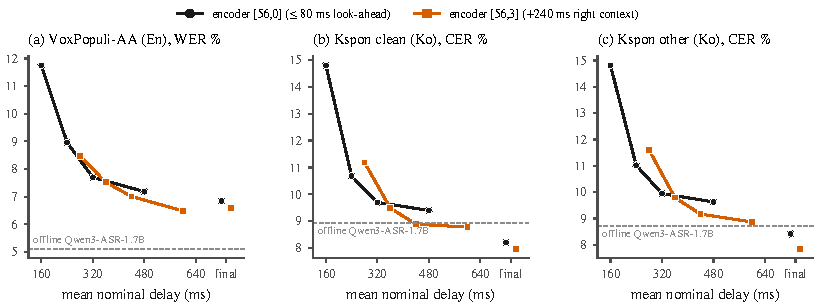
\includegraphics{figures/figA6_backbone_lookahead.pdf}
  \caption{Encoder look-ahead versus decoder delay in the streaming backbone (Stage-1 pilot, 1.7B thinker): error rate against mean nominal delay with encoder context $[56,0]$ (look-ahead ${\le}\,80$\,ms; black circles) and $[56,3]$ (240\,ms more right context; vermillion squares) for $\delta=2,3,4,6$, and in final mode; dashed: offline Qwen3-ASR-1.7B. (a)~VoxPopuli-AA WER (English); (b)~KsponSpeech eval\_clean and (c)~eval\_other CER (Korean). The nominal delay is $80\delta$\,ms for $[56,0]$ and $80\delta+120$\,ms for $[56,3]$. One checkpoint, trained with sampled encoder contexts, is evaluated at both settings. At matched mean delay, encoder look-ahead and decoder delay are largely interchangeable.}
  \label{fig:backbone}
\end{figure}

\paragraph{Backbone results.}
\Cref{tab:backbone} compares the two Stage-1 pilots with two earlier 0.6B models and two references. The earlier recipe trained a 0.6B model in several stages on 5.6k\,h of English and Korean ASR data with $\delta\in\{2,3,4,6\}$ and without final mode; the second earlier model fine-tunes it with sentence-level commit tokens while the encoder is frozen. At $\delta=4$ and $\delta=6$, the 1.7B pilot improves on these two models by 10--24\% and 19--22\% (relative), all significant; only at $\delta=2$ on KsponSpeech is the commit-token model better, by 0.7--1.0 points. Against the 0.6B pilot, the 1.7B thinker is 6--11\% better in every Korean comparison, on par in English streaming, and 4\% better in English final mode (6.84 vs.\ 7.14\%; difference $-0.31$ points, 95\% CI $[-0.57,-0.03]$). Against the released Nemotron~3.5 model at $[56,0]$ (the encoder we start from, with its own causal RNN-T decoder), the English gap closes as $\delta$ grows: $+4.87$ points (+70.8\%) at $\delta=2$, $+0.82$ (+12.0\%) at $\delta=4$, $+0.30$ (n.s.) at $\delta=6$ and $-0.04$ (n.s.) in final mode. On KsponSpeech, the backbone is 24.0\% ($\delta=2$) to 57.8\% (final mode) better on eval\_clean and 11.9\% to 49.9\% better on eval\_other. In final mode, it beats offline Qwen3-ASR-1.7B on KsponSpeech eval\_clean (8.21 vs.\ 8.92\%; $-0.71$ points, $[-1.05,-0.37]$), matches it on eval\_other (8.42 vs.\ 8.71\%, n.s.) and trails it in English by 1.73 points (6.84 vs.\ 5.10\%, +33.9\%).

\paragraph{Caveats.}
These are single-speaker results. VoxPopuli-AA is not speaker-disjoint from our training data, because the official VoxPopuli split is not: 80 of its 207 speakers and 280 of its 292 sessions also occur in training, although no utterance or sentence is duplicated. AA-WER only approximates the published scoring. The final-mode gain over offline Qwen3-ASR on KsponSpeech may be an in-domain effect, since the KsponSpeech training set is part of our data. The training data contain no German, and the backbone has not been evaluated on telephone-band \taxi speech or on two-speaker mixtures, so none of these numbers carries over to \task.

\paragraph{Encoder look-ahead versus decoder delay.}
Latency can be bought with encoder right context or with decoder delay. As the 1.7B pilot was trained with sampled contexts, we evaluate the same checkpoint at $[56,0]$ and $[56,3]$ (\cref{fig:backbone}) and compare the two at their mean nominal delay: $80\delta$\,ms for $[56,0]$ and $80\delta+120$\,ms for $[56,3]$, whose explicit right context adds 120\,ms on average and 240\,ms at most. Below, a difference is the error of $[56,3]$ minus that of $[56,0]$ in points, given as VoxPopuli-AA WER\,/\,KsponSpeech eval\_clean CER\,/\,eval\_other CER, with significance from the paired bootstrap. Between 240 and 320\,ms the evidence is mixed: $[56,3]$ at $\delta=2$ (280\,ms) is better in English than $[56,0]$ at $\delta=3$ (240\,ms) but worse in Korean ($-0.49/+0.51/+0.58$, all significant), and worse everywhere than $[56,0]$ at $\delta=4$ (320\,ms; $+0.77/+1.49/+1.65$, all significant). Between 320 and 480\,ms the two are interchangeable: $[56,3]$ at $\delta=3$ (360\,ms) differs from $[56,0]$ at $\delta=4$ (320\,ms) by $-0.18/-0.21/-0.14$ and from $[56,0]$ at $\delta=6$ (480\,ms) by $+0.34/+0.09/+0.17$, none significant. Right context helps from 440\,ms on ($[56,3]$ at $\delta=4$ vs.\ $[56,0]$ at $\delta=6$: $-0.17$ (n.s.)$/-0.51/-0.46$; at equal $\delta=6$, i.e.\ 600 vs.\ 480\,ms: $-0.70/-0.62/-0.76$, significant) and in final mode ($-0.25/-0.25/-0.58$, all significant), and matching the maximum rather than the mean delay would shrink these gains further. We therefore keep the causal $[56,0]$ and let $\delta$ set the latency, which \model conditions separately for each stream.


% =====================================================================
% Appendix G: translation-unit pilot (one-column appendix).
% Ko<->En numbers (Blocks A, B; Figs. A8, A9) are measured and come from the
% archived score and analysis files of the pilot. Not cited on purpose (raw
% outputs not archived): oracle-LAAL ranges, collapse-free re-scores and
% duplicate re-emission counts. Block C (En<->De on TAXI) is planned.
% Do not claim significance, transfer to speech input, trained models or TAXI,
% that SEM_END beats the utterance end, or that the BLEU loss is paraphrase.
% =====================================================================
\section{Translation-Unit Pilot}\label{app:units}

This appendix reports a text-level pilot that motivates the translation commit units of \model (\cref{sec:model}). Its conditions differ from those of the benchmark: it simulates simultaneous translation over gold transcripts with gold word end times; it uses single-speaker Korean and English utterances from monolingual ASR corpora (150 per direction for quality, 300 per language for alignment statistics), not dialogues and not \pair{En}{De}; Qwen3.8-27B is the incremental translator; the references are offline translations by EXAONE-4.0-32B (silver references); and latency is computation-unaware LAAL on the gold word times. The pilot compares commit units under these conditions only and does not predict results for speech input, for trained models or on \taxi.

\paragraph{Commit policies.}
Let $u_{1:n}$ be the gold transcript of an utterance, $e_i$ the end time of word $u_i$, and $v_{1:J}$ the full offline translation by a teacher LLM. A policy commits translation text after it has read $b$ source words, and committed text is never revised, unlike in re-translation \citep{arivazhagan2020retranslation}. We compare four policies.
(i)~\emph{Utterance end} commits once, after $u_n$, which amounts to offline translation of the utterance.
(ii)~\emph{SEM\_END} commits at sentence-level semantic-completion boundaries: the positions at which an existing LLM-based labeller, which sees only the source transcript, judges the transcript so far semantically complete, i.e., later words will not change its meaning (in practice mostly the sentence-final punctuation of the transcript); the utterance end is added. These boundaries do not depend on the target language.
(iii)~\emph{Alignment-only meaning units (MU).} Contextual alignment \citep{labiausse2025highfidelity} assigns each target word $v_j$ to the source position $\alpha_j=\arg\max_{1\le i\le n}\,[L_j(i)-L_j(i-1)]$, where $L_j(i)$ is the summed log-probability of the tokens of $v_j$ when $v_{1:J}$ is force-decoded from $u_{1:i}$; ties go to the earliest $i$. A position $i$ is a \emph{valid cut} if the target words aligned at or before $i$ form a prefix $v_{1:k}$, so that, relative to the teacher's translation, the output up to that point need not change later. An \emph{MU boundary} is a valid cut that covers more target words than the previous valid cut; $n$ is always a valid cut and an MU boundary. This approximates, with alignment instead of generation, the translation-prefix consistency that defines meaning units (``meaningful units'' in \citealp{zhang2020learning}): minimal source segments whose translation is a prefix of the full translation. The policy commits at every MU boundary.
(iv)~\emph{Verified meaning units (MU2)} commit at a subset of the valid cuts. A candidate is a valid cut $b<n$ that covers more target words than the last commit $b'$ and lies at least a minimum unit after it: 2 Korean eojeol (space-delimited words) or 3 English words, and $e_b-e_{b'}\ge1.0$\,s. At a candidate, the translator receives the source heard so far and the committed translation in its prompt, rather than as a forced prefix, and writes only the new text. A language guard regenerates once and then rejects output in the wrong script: Han or Kana characters, Hangul in English output, or less than 30\% Hangul in Korean output. A generation check, in the spirit of \citet{zhang2020learning}, accepts the new text only if its sentence-level chrF \citep{popovic2015chrf} against the newly covered span $v_{k'+1:k}$ of the teacher's translation is at least $\theta=50$, where $k'$ is the coverage at the last commit. The rest of the utterance is translated at its end.

\paragraph{Setup.}
We sample 300 utterances per source language with word end times from monolingual Korean and English ASR corpora, plus a second, independent sample of the same size to check sample dependence; the source text is the gold transcript, and the SEM\_END positions are the labeller's output for it. The labeller has LLM judges rate candidate positions, proposed by an LLM or by rules (e.g., at sentence-final punctuation), and keeps a candidate if its ratings pass thresholds set per candidate type so that precision against LLM-annotated reference labels is at least 0.90 on a development split. Alignments come from Qwen3.8-27B on both samples and from EXAONE-4.0-32B on the first. The quality runs use 150 utterances per direction from the first sample (mean length 11.09\,s for Korean and 15.05\,s for English sources), with Qwen3.8-27B as translator and as the MU2 teacher. The references are EXAONE-4.0-32B offline translations of the full gold transcripts, from another model family than the translator; no human references exist for these utterances. Teachers and reference translator receive \textit{``Translate the following $\langle$src$\rangle$ speech transcript into natural $\langle$tgt$\rangle$. Output only the $\langle$tgt$\rangle$ translation, nothing else.''}, followed by the transcript.
\draftnote{name the source corpora, the sampling arguments and the origin of the word times; the Korean transcripts seem to be filtered ASR output, so verify before calling them gold}

Block A of \cref{tab:units} runs the utterance end, SEM\_END and MU2 with one incremental prompt and the language guard; only MU2 adds the minimum unit and the generation check. The prompt reads
\begin{quote}\small\itshape
You are a simultaneous interpreter translating $\langle$src$\rangle$ speech into $\langle$tgt$\rangle$.\\
Source heard so far: $\langle$source prefix$\rangle$\\
Translation already given (cannot be changed): $\langle$committed text, or ``(none)''$\rangle$\\
Translate only the part of the source that the translation already given does not cover yet, continuing it naturally in $\langle$tgt$\rangle$. [The speaker is still talking: translate only what has been said so far and do not guess the rest.] Output only the new $\langle$tgt$\rangle$ text, nothing else. If nothing new can be translated yet, output nothing.
\end{quote}
where the bracketed sentence appears only before the end of the utterance, and a regeneration by the guard appends \textit{``Write the answer in $\langle$tgt$\rangle$ only.''} Block B runs the utterance end, SEM\_END and alignment-only MUs with the offline prompt, which before the end of the utterance also says \textit{``The transcript may be incomplete because the speaker is still talking: translate only what has been said so far, do not guess or complete the rest.''}; the committed text is forced as the beginning of the answer, and the continuation is committed. Block B has no language guard, and its latency was not reported. In both blocks, the utterance-end translation may use up to 160 tokens and every other step at most $\min(160,\,2\ell+8)$, where $\ell$ is the token length of the utterance-end translation, and an $m$-gram ($m\le3$) repeated three or more times in a row is cut.

We report corpus BLEU \citep{papineni2002bleu} and chrF with sacreBLEU \citep{post2018call}, with the BLEU tokenizer \texttt{intl} for Korean and \texttt{13a} for English output; chrF is primary for Korean output. An output \emph{collapses} if it is empty, is in the wrong script as defined for the guard, or contains an $m$-gram ($m\le3$) repeated three or more times in a row. Latency ignores LLM computation and ASR delay. Output word $j$ gets the commit time $d_j=e_b$ of the step that wrote it, and per utterance
\[
  \mathrm{LAAL}=\frac{1}{\tau}\sum_{j=1}^{\tau}\Bigl(d_j-(j-1)\,\frac{e_n}{|Y|}\Bigr),
\]
where $|Y|$ is the output length in words and $\tau$ the first $j$ with $d_j=e_n$ (or $|Y|$ if there is none). This is the length-adaptive form \citep{papi2022overgeneration} of Average Lagging \citep{ma2019stacl}, except that $|Y|$ replaces $\max(|Y|,|Y^*|)$ with the reference length $|Y^*|$; the two agree whenever the output is at least as long as the reference. \emph{First commit} is $d_1$. Both are averaged over utterances, so the LAAL of the utterance end equals the mean utterance length.
\draftnote{recompute LAAL with $\max(|Y|,|Y^*|)$ when the raw outputs are re-exported}
For the alignment statistics, a source word $u_i$ waits $e_{b(i)}-e_i$ until the first boundary $b(i)\ge i$ of a policy.

% =====================================================================
% Table A10 (tab:units): text-level commit-unit pilot. Included from App. G.
% Blocks A and B (Ko<->En) are measured: values copied from the archived score
% files of the pilot (prompt-based run = Block A; forced-prefix run = Block B).
% Block B: no latency was reported, nor collapse counts for its utterance-end
% and SEM_END rows ("--").
% Block C (En<->De on TAXI gold transcripts) is planned: every cell is \tbd.
% =====================================================================
\begin{table}[t]
  \caption{Text-level commit-unit pilot (\cref{app:units}). Blocks A and B: \pair{Ko}{En}, 150 single-speaker utterances per direction, fixed transcripts (Korean: ASR output kept when two recognisers agree) with forced-aligned word end times, Qwen3.8-27B as translator, silver references (offline EXAONE-4.0-32B translations) and computation-unaware LAAL. The two blocks use different prompts, so rows are compared only within a block. Block C (planned): \pair{En}{De} \taxi turns with gold transcripts and forced-aligned word times, scored by \scorer against the human references; its left group is \deen, its right group \ende, and its LAAL is \laal on the ideal clock. LAAL and First (commit time of the first output word) in seconds. Coll.: collapsed outputs (empty, wrong script or a repetition loop), out of 150 in Blocks A and B. Candidates accepted: MU2 candidates that pass the language guard and the chrF check. --: not reported; blank: pending.}
  \label{tab:units}
  \centering
  \small
  \setlength{\tabcolsep}{4.5pt}
  \begin{tabular}{@{}lcccccccccc@{}}
    \toprule
    & \multicolumn{5}{c}{\koen (C: \deen)} & \multicolumn{5}{c}{\enko (C: \ende)} \\
    \cmidrule(lr){2-6}\cmidrule(l){7-11}
    Block\,/\,commit policy & BLEU & chrF & LAAL & First & Coll. & BLEU & chrF & LAAL & First & Coll. \\
    \midrule
    \multicolumn{11}{@{}l}{\textit{A: prompt-based commits}} \\
    Utterance end             & 35.2 & 61.3 & 11.09 & 11.09 & 0 & 23.4 & 44.2 & 15.05 & 15.05 & 1 \\
    SEM\_END                  & 35.3 & 61.1 &  7.49 &  8.23 & 0 & 22.4 & 43.7 &  8.63 &  9.74 & 0 \\
    Verified MU (MU2)         & 31.1 & 60.2 &  5.19 &  7.03 & 0 & 19.9 & 42.0 &  7.33 &  8.25 & 1 \\
    \quad candidates accepted & \multicolumn{5}{c}{197/368 (54\%)} & \multicolumn{5}{c}{185/873 (21\%)} \\
    \midrule
    \multicolumn{11}{@{}l}{\textit{B: forced-prefix continuation (latency not reported)}} \\
    Utterance end             & 32.9 & 58.4 & -- & -- & -- & 21.2 & 42.3 & -- & -- & -- \\
    SEM\_END                  & 34.4 & 59.2 & -- & -- & -- & 19.2 & 40.8 & -- & -- & -- \\
    Alignment-only MU         & 28.1 & 54.2 & -- & -- & 5  & 12.9 & 33.1 & -- & -- & 31 \\
    \midrule
    \multicolumn{11}{@{}l}{\textit{C: \pair{En}{De} \taxi turns, human references (planned)}} \\
    Turn end                  & \tbd & \tbd & \tbd & \tbd & \tbd & \tbd & \tbd & \tbd & \tbd & \tbd \\
    Verified MU (MU2)         & \tbd & \tbd & \tbd & \tbd & \tbd & \tbd & \tbd & \tbd & \tbd & \tbd \\
    \quad candidates accepted & \multicolumn{5}{c}{\tbd} & \multicolumn{5}{c}{\tbd} \\
    \bottomrule
  \end{tabular}
\end{table}


\paragraph{Verified meaning units halve the lag.}
In Block A (\cref{tab:units,fig:units}), MU2 roughly halves LAAL relative to the utterance end, from 11.09 to 5.19\,s (\koen) and from 15.05 to 7.33\,s (\enko), stays below SEM\_END (7.49 and 8.63\,s), and makes its first commit earlier (7.03 against 11.09\,s and 8.25 against 15.05\,s). chrF falls from 61.3 to 60.2 and from 44.2 to 42.0; BLEU falls more, from 35.2 to 31.1 and from 23.4 to 19.9. Whether this reflects paraphrase or errors is untested, since the references are silver and no human judged the outputs. SEM\_END scores close to the utterance end, but its output is identical to the utterance-end output in 96/150 (\koen) and 83/150 (\enko) utterances.

\begin{figure}[t]
  \centering
  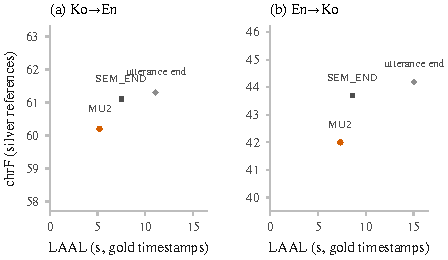
\includegraphics{figures/figA8_unit_quality_latency.pdf}
  \caption{Commit-unit pilot, Block A of \cref{tab:units}: chrF against computation-unaware LAAL for (a)~\koen and (b)~\enko (text level; 150 utterances per direction; gold transcripts and word times; silver references). Verified meaning units (MU2) roughly halve LAAL relative to committing at the utterance end, at a small chrF cost; SEM\_END lies in between on both axes. The LAAL of the utterance end equals the mean utterance length.}
  \label{fig:units}
\end{figure}

\paragraph{SEM\_END is sentence-level.}
Across the three alignment runs, an utterance contains 1.16--1.44 SEM\_END units against 3.09--3.45 MUs for Korean sources, and 1.75--1.88 against 5.52--5.73 for English sources. A SEM\_END unit spans 11.83--12.82 eojeol against 5.70--6.73 for an MU in Korean, and 24.68--26.15 against 9.22--9.93 words in English (\cref{fig:unit-gran}). Of all SEM\_END positions, 42.3--85.9\% coincide with the utterance end, which is a valid cut by definition; counting these, 79.6--92.2\% are valid cuts. Yet SEM\_END positions cover only 2.0--8.1\% of the MU boundaries inside utterances, and a source word waits 3.75--4.05\,s (Korean) and 5.20--5.73\,s (English) for the next SEM\_END boundary, against 2.59--3.25\,s and 3.22--3.38\,s for the next MU boundary. Semantic completion of the source therefore marks few of the points at which a translation could already be committed.
\draftnote{also report the valid-cut share of the SEM\_END positions inside utterances}

\begin{figure}[t]
  \centering
  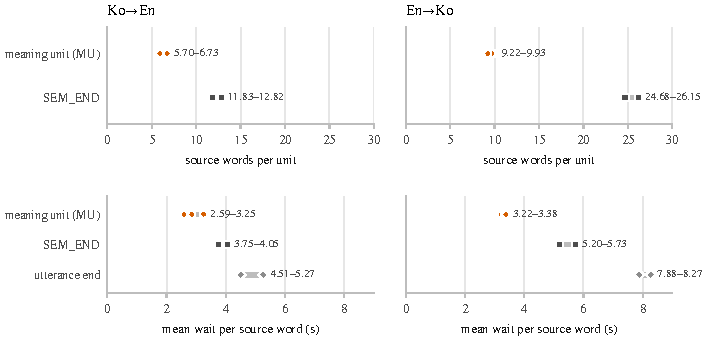
\includegraphics{figures/figA9_unit_granularity.pdf}
  \caption{Unit granularity on 300 utterances per source language: source words per unit (Korean: eojeol) and mean wait of a source word until the next commit boundary, for alignment-only meaning units (MU), SEM\_END and the utterance end. Dots are three alignment runs (Qwen3.8-27B and EXAONE-4.0-32B on one sample; Qwen3.8-27B on a second sample); bars span the minimum to the maximum. SEM\_END and utterance-end values depend on the sample but not on the teacher.}
  \label{fig:unit-gran}
\end{figure}

\paragraph{Unverified units collapse, and acceptance depends on the direction.}
Block B commits without verification: alignment-only MUs continued from a forced prefix collapse in 5/150 \koen and 31/150 \enko outputs, through text in another script (including copied source), loops or empty output, and their chrF drops to 54.2 and 33.1, against 58.4 and 42.3 for the utterance end of the same block. MU2 collapses in 0/150 and 1/150 utterances; the single \enko case is an utterance whose utterance-end output is empty as well. MU2 differs from Block B's MUs in its prompt, the guard, the minimum unit and the check at once, so the pilot does not separate their effects. The check accepts 197 of 368 candidates (54\%) for \koen but only 185 of 873 (21\%) for \enko; nearly all rejections fail the chrF threshold (171 and 685; the other three \enko rejections are one empty and two wrong-language outputs). This is consistent with Korean word order: a Korean translation places the verb last, so the translation of an English prefix rarely matches the span of the full translation aligned to it. With so few accepted candidates, \enko MU2 is only 1.3\,s faster than SEM\_END, and its output equals the utterance-end output in 52/150 utterances (32/150 for \koen).

\paragraph{Extension to \pair{En}{De}.}
Block C of \cref{tab:units} repeats the comparison on the main pair with human references: \taxi turns with gold transcripts and forced-aligned word times, Qwen3.8-27B as alignment teacher and translator, $\theta=50$, a German minimum unit set on held-out data, and trimming of committed text that is re-emitted at the turn end; \scorer scores the output against the TAXI references. Its MU2 row is the oracle-transcript streaming bound of \cref{tab:main}. TAXI turns are much shorter than the pilot utterances (mean source turn 3.086\,s in German and 4.624\,s in English; mean pilot utterance 11.09\,s in Korean and 15.05\,s in English), which bounds what commits inside a turn can gain.
\draftnote{planned; Block C has not been run}

\paragraph{Limitations.}
The references are silver translations by one LLM, with no human references, COMET or human judgement. The utterances are long, come from single-speaker monolingual corpora and are not dialogues. Transcripts and word times are gold, latency ignores computation and ASR delay, and LAAL is computed per utterance rather than as session-level \laal. There are no confidence intervals: with 150 utterances per direction, small differences, such as between SEM\_END and the utterance end, are not interpreted. The translator, the alignment teacher and the target of the generation check are the same model (Qwen3.8-27B), so the check may favour its own phrasing, and neither $\theta$ nor the minimum unit was tuned. Finally, MU2 sometimes re-emits committed text at the utterance end; the pilot does not trim it, which may inflate the \koen length ratio of MU2 (1.13, against 1.05 for the utterance end).

% =====================================================================
% Appendix H: statistics, licences and reproducibility (one-column appendix).
% The statistical protocol is the planned design (the v0.1 scorer computes no
% intervals yet). Measured facts used here: 86 sessions, about 3.3k reference
% words per direction, the 86/86 rebuild match (App. A). Licence entries follow
% the outline and must be verified against the licence texts.
% The main comparisons follow Sec. 6.5: the decoupled twin and the
% same-backbone cascade are the tests of coupling. The human-interpreter
% reference point moved here from Sec. 7 (round 1); for space, Sec. 7 no
% longer points to it (Sec. 6.2 could). Rank agreement uses tau_b within
% direction x wrapper strata as defined in App. C (tab:validity). Table A12
% (tab:licences) is input near the top so that it does not drift into App. I.
% =====================================================================
\section{Statistics, Licences and Reproducibility}\label{app:repro}

\taxi has 86 sessions and about 3.3k reference words per direction, so every result on \bench comes with an uncertainty estimate, and the statistical protocol below is fixed before the test runs.
\draftnote{planned: the v0.1 scorer reports no intervals yet; the bootstrap, the Holm correction and the minimum detectable differences are being added; the preliminary runs reported so far predate this protocol and will be re-run under it}

% Input early so that the float stays inside this appendix (it is referenced
% from the Impact Statement, App. A, App. B and the Licences paragraph below).
% =====================================================================
% Table A12 (tab:licences): licences, use and release of the corpora,
% generation models and services behind CST-Bench and Model. Included from
% App. H. Baseline systems and their licences are in tab:baselines (App. D);
% scoring, alignment and QA models are not listed (see the caption).
% Placed [htbp] so that it can follow App. H's text instead of leaving a
% mostly empty page. Licence spelling: SPDX (Apache-2.0).
% Every entry must be checked against the licence text before submission;
% the licences of the backbone training corpora are not yet listed (only
% Switchboard's LDC licence is recorded), so that cell names no licence and
% none is guessed. The row cites the corpora that have verified bib entries
% (LibriSpeech, VoxPopuli, KsponSpeech, MUSAN, DEMAND); Granary-YODAS,
% Switchboard, NIKL, AI Hub, ETSI noise and Qwen3.8-27B have none yet.
% Baselines (incl. the optional Hibiki-Zero, CC BY-NC-SA 4.0) are in
% tab:baselines, not here.
% =====================================================================
\begin{table}[htbp]
  \caption{Licences and terms of the corpora, generation models and services behind \bench and \model, how we use them, and what we release. Baseline systems are listed in \cref{tab:baselines}; scoring, alignment and quality-control models (\cref{app:scorer,app:syn}) are used unchanged under their own licences and are not redistributed. $^\ast$Planned: \syn and the \model weights do not exist yet.}
  \label{tab:licences}
  \centering
  \footnotesize
  \setlength{\tabcolsep}{4pt}
  \begin{tabular}{@{}>{\raggedright\arraybackslash}p{3.35cm}>{\raggedright\arraybackslash}p{4.1cm}>{\raggedright\arraybackslash}p{4.4cm}>{\raggedright\arraybackslash}p{4.4cm}@{}}
    \toprule
    Asset & Licence\,/\,terms & How we use it & Released by us \\
    \midrule
    BAS TAXI 2.5 \citep{bas2001taxi,reichel2016bas}
      & Scientific licence, free of charge (commercial licence available); no redistribution, even in part, without the written permission of the copyright holders
      & \taxi, the real test track; evaluation only
      & Session and turn IDs, configurations, build scripts, checksums, per-turn scores keyed by turn ID; no audio, text or system output \\
    \addlinespace[1pt]
    XDailyDialog \citep{liu2023xdailydialog}
      & CC BY-NC-SA 4.0
      & \syn dialogues and English--German references; evaluation only
      & XDailyDialog-based \syn subset under CC BY-NC-SA 4.0$^\ast$ \\
    \addlinespace[1pt]
    BConTrasT \citep{farajian2020findings}, built on Taskmaster-1 \citep{byrne2019taskmaster}
      & CC BY-SA 4.0 (Taskmaster-1: CC BY 4.0)
      & \syn dialogues and English--German references; evaluation only
      & BConTrasT-based \syn subset under CC BY-SA 4.0$^\ast$ \\
    \addlinespace[1pt]
    Nemotron 3.5 ASR Streaming 0.6B \citep{nvidia2026nemotron35asr}
      & OpenMDW-1.1
      & Streaming encoder of \model, fine-tuned
      & Encoder within the \model weights, under OpenMDW-1.1$^\ast$ \\
    \addlinespace[1pt]
    Qwen3-ASR \citep{shi2026qwen3asr}
      & Apache-2.0
      & Thinker LM of \model (1.7B; its audio encoder removed); Qwen3-ASR-1.7B in cascade baselines and for \syn re-recognition
      & Thinker within the \model weights, under Apache-2.0$^\ast$ \\
    \addlinespace[1pt]
    Backbone training corpora (\cref{app:model}): LibriSpeech \citep{panayotov2015librispeech}, VoxPopuli \citep{wang2021voxpopuli}, Granary-YODAS, Switchboard, KsponSpeech \citep{bang2020ksponspeech}, NIKL, AI~Hub, a curated pool; MUSAN \citep{snyder2015musan}, DEMAND \citep{thiemann2013demand} and ETSI noise
      & Terms of each corpus (Switchboard: LDC licence)
      & Training (Stages 0--1) and augmentation of the \model backbone; one KsponSpeech transcript is quoted in \cref{fig:delta-delay}
      & No data; only the \model weights trained on them$^\ast$ \\
    \addlinespace[1pt]
    Qwen3.8-27B
      & Apache-2.0
      & MT in cascade baselines; alignment, translation and verification teacher of the MU2 commit targets; one of three translators of the \syn Korean text
      & Per-turn scores of its runs; none of its translations as references \\
    \addlinespace[1pt]
    MADLAD-400-10B-MT \citep{kudugunta2023madlad}
      & Apache-2.0
      & One of three translators of the \syn Korean text
      & Korean text of \syn{}$^\ast$ \\
    \addlinespace[1pt]
    EXAONE-4.0 \citep{lgai2025exaone4}
      & EXAONE AI Model License: non-commercial; outputs may not be used to develop competing models
      & Internal evaluation only: agreement check of the \syn Korean text; references and second alignment teacher in the pilot of \cref{app:units}
      & Nothing; its outputs are neither released nor used for training \\
    \addlinespace[1pt]
    Azure neural TTS \citep{microsoft2026text}
      & Service terms of the provider; synthesis on a paid pay-as-you-go resource only, as statements on the free tier conflict
      & Commercial \syn edition (main results)
      & Audio of this edition$^\ast$ \\
    \addlinespace[1pt]
    CosyVoice~3 \citep{du2025cosyvoice3} or Qwen3-TTS \citep{hu2026qwen3tts}
      & Apache-2.0 (weights)
      & Open \syn edition on a subset (rank agreement)
      & Audio of this edition$^\ast$ \\
    \addlinespace[1pt]
    \texttt{cst-bench} code and \scorer
      & Apache-2.0
      & Building \taxi and \syn; scoring every system
      & All code, configurations, checksums and wrappers \\
    \bottomrule
  \end{tabular}
  % (integrator) The draft note on verifying these entries now follows the
  % Licences paragraph of App. H, so that the float fits the page in both builds.
\end{table}


\paragraph{Session-clustered paired bootstrap.}
We resample sessions rather than turns, because the turns of one session share speakers, topic and context, and resampling them independently would understate the variance. Each of 2,000 resamples draws the sessions of a test set with replacement and keeps every turn of a drawn session. Every metric is recomputed on each resample exactly as on the full test set: BLEU and chrF from the statistics pooled over the resampled turns, COMET over the resampled turns, latency statistics over the resampled non-empty turns, and error rates from pooled counts; per-session scores are never averaged. A 95\% interval spans the 2.5th to the 97.5th percentile of the resampled values. A paired comparison scores both systems on the same resamples \citep{koehn2004statistical}, and its two-sided $p$-value is twice the smaller fraction of resampled differences on either side of zero. On \syn, the resampling unit is the source dialogue, so both speaker--language assignments of a dialogue are drawn together.

\paragraph{Main comparisons and multiple testing.}
Before the test runs, we fix the main comparisons, the operating point of every system (chosen on the \syn calibration split; \cref{app:baselines}) and the decision rules. The main comparisons are oracle against realistic segmentation for each system and direction (RQ1; \cref{sec:intro}), and \model against the decoupled twin and against the same-backbone cascade, the two tests of coupling turn-taking and translation (\cref{sec:exp-ablation}). Holm's step-down procedure \citep{holm1979simple} controls the family-wise error rate over them at 0.05. Every other difference is reported with its interval but is not tested.

\paragraph{Rank agreement.}
Kendall's $\tau_b$, computed within direction and wrapper strata and averaged (\cref{app:scorer}), compares system rankings between \taxi and \syn, between the two TTS editions, between gold and silver references, across render seeds and between metrics (\cref{tab:validity}). Its 95\% interval comes from the same bootstrap: sessions of different test sets are drawn independently, two metrics on one test set share each draw, and $\tau_b$ is recomputed on every resample. The decision rule for the agreement between \syn and \taxi, a threshold $\tau^\ast$, is fixed before the test runs, and a low $\tau_b$ is reported as a finding.

\paragraph{Minimum detectable difference.}
For each metric and direction, we compute the smallest paired difference that the test detects at a two-sided level of 0.05 with a power of 0.8, $\mathrm{MDD}=(z_{0.975}+z_{0.8})\,\hat\sigma_\Delta\approx2.80\,\hat\sigma_\Delta$, where $\hat\sigma_\Delta$ is the session-bootstrap standard error of a paired difference, estimated from the variance of \taxi segment scores. On \taxi, the MDDs for \ende and \deen are \tbdtext{} and \tbdtext{} COMET points, \tbdtext{} and \tbdtext{} chrF points, and \tbdtext{} and \tbdtext{}\,s of median \eo. We do not interpret smaller differences and use the same estimate to size \syn (\cref{app:syn}).

\paragraph{Human reference point.}
Human interpreters are a reference point for our latencies, not a target: their English-to-Korean ear-voice span is about 3\,s \citep{lee2002ear}, and we evaluate no human interpretation.

\paragraph{Release.}
We release one Apache-2.0 package with the \taxi build scripts, frozen configurations and checksums, the session renderer, \scorer and the oracle and realistic wrappers of every baseline (\cref{app:baselines}), together with the per-turn scores of every system keyed by turn ID. TAXI itself is never redistributed. Users obtain the corpus from BAS under its licence \citep{bas2001taxi,reichel2016bas} and rebuild the track deterministically; \cref{app:taxi} gives the commands and the verification of timeline digests and audio hashes, and a local rebuild matched 86/86 timeline digests and audio hashes in each L0 configuration. The per-turn scores let anyone who holds the corpus compare new systems with ours without access to our outputs. No TAXI audio, transcript, translation or system output appears in the release or in this paper; apart from one transcript from KsponSpeech \citep{bang2020ksponspeech} in \cref{fig:delta-delay}, all text examples are invented. \syn is released as two subsets under the licences of their sources, with a data card (\cref{app:syn}). The \model weights carry both component licences: OpenMDW-1.1 for the encoder and Apache-2.0 for the thinker.
\draftnote{planned: the realistic wrappers, \syn and the \model weights do not exist yet}

\paragraph{Exact configurations.}
Every baseline is pinned to a public checkpoint and version (\cref{tab:baselines}); the training stages, data and hyperparameters of \model are listed in \cref{tab:training}; render seeds derive from session IDs (\cref{app:taxi}); and computation-aware latency is measured on one fixed hardware configuration (\cref{tab:ca-latency}). We report sacreBLEU signatures \citep{post2018call} and the COMET checkpoint (wmt22-comet-da; \citealp{rei2022comet}), and we pin every package that changes scores, including the number normaliser. For review, an anonymised copy of the code is available at \tbdtext{}.
\draftnote{planned; pin the number normaliser and add the anonymised link}

\paragraph{Licences.}
\Cref{tab:licences} lists the corpora, generation models and services behind \bench and \model, their licences or terms, how we use them and what we release. Three constraints shape the release: TAXI may not be redistributed; the two \syn sources carry incompatible ShareAlike licences, hence two subsets; and the EXAONE AI Model License restricts EXAONE-4.0 outputs to non-commercial use, so we use them only internally (the agreement check of the \syn Korean text and the pilot of \cref{app:units}) and neither release them nor train on them. The commercial \syn edition is synthesised only on a paid Azure resource. No corpus used to train \model is redistributed.
\draftnote{decision needed: list the licence of each training corpus of \cref{app:model} (the licence of at least one Korean set in the curated pool is unknown) and confirm that these terms allow releasing weights trained on them}
\draftnote{\cref{tab:licences}: verify every entry, the TAXI copyright holders and the Azure output terms against the current licence texts before submission; decision needed: the licences of the backbone training data (at least one Korean set of the curated pool has an unknown licence), whether they allow releasing the \model weights, and whether the KsponSpeech terms allow quoting a transcript}


\end{document}
